\section{The Modified Queuing Model}\label{ch:queue_model}
Using the data collected, a model for simulating the LOB is created. It is based on the one developed by \cite{A6} but with several important modifications. The LOB is again represented as a $2K$-dimensional vector $$Q(t) = (Q_{-K}(t), \ldots Q_{-1}(t), Q_1(t), \ldots , Q_K(t))$$ centered around $p_0$. Events at each position $k$ cause either a positive or negative change in $Q_k(t)$. The magnitudes of the events are distributed exponentially with means $\mu^+_k$ and $\mu^-_k$ respectively. That is, if a positive event occurs at time $t$ with size $e$, set $q(t) \leftarrow q(t) + e$, and if a negative event occurs at time $t$ with size $e$, set $q(t) \leftarrow (q(t) - e)^+$ where $b^+ = 0$ if $b < 0$ and $b$ otherwise (so as to keep the queue size non-negative). An exception occurs when a negative order occurs at the best bid or ask price. It is assumed to be a market order that will consume liquidity from successive prices until it is filled. If the size of the event is larger than the volume at the best price, the leftover part of the order is filled with the next best price and so on. The arrivals of events are modelled as a multivariate Poisson process. With positive and negative arrivals at each of the $2K$ positions, there are $4K$ such processes. The marginal arrival process at each position is a Poisson process with positive and negative arrivals having mean rates $\lambda^+_k$ and $\lambda^-_k$ respectively. Arrivals are simulated in chunks of length $t$. Let $N^+_k(t)$ be the number of positive arrivals at position $k$ ($N^-_k(t)$ for negative arrivals) during a time period of length $t$. Then, the arrivals have a $4K\times4K$ correlation matrix $R$ where $R_{i+,j+} = corr(N^+_i(t), N^+_j(t))$, $R_{i+,j-} = corr(N^+_i(t), N^-_j(t))$, $R_{i-,j+} = corr(N^-_i(t), N^+_j(t))$, and $R_{i-,j-} = corr(N^-_i(t), N^-_j(t))$.

There are several differences between this model and the queue-reactive model developed by \cite{A6}. Modifications were made to better fit observations from the dataset. First, the sizes of positive and negative events are not just the $AES$'s, but rather exponential random variable variables with means equal to the $AES$'s. This adjustment was made because the event sizes exhibit considerable variation. Section \ref{ch:event_sizes} shows that an exponential distribution reasonably fits the distribution of event sizes. Although it may not fit the data completely, it is the easiest part of the model to adjust.

Second, the rate of arrival of events at a given position does not vary as the size of the queue changes. In the data set, the queue sizes varied widely (sometimes several dozens multiplies of the $AES$'s) and no substantial change in rate was observed when the queue sizes changed. It is possible that the rates differ in a predictable way as the queue sizes changes, but there were not enough data points to observe reliable differences, especially in intermediate sizes where there was no data at all. This change also has the added benefit of simplifying the model greatly.

Third, arrival processes are modelled as a multivariate Poisson process instead of independent Poisson processes. In Section \ref{ch:poisson}, the claim that the arrival rates at each position reasonably follow individual Poisson processes is validated. However, Section \ref{ch:correlations} finds that these processes are significantly correlated. A multivariate Poisson process allows these correlations to be incorporated in the simulation.

\section{Building An Abbreviated Order Book}
To facilitate analysis, steps were taken to clean the raw data. Often in the data set, several updates that have the same magnitude, sign, and inter-arrival time occur in quick succession. These orders were likely made by a trader who split up a larger trade. As it should represent one trade, orders that occur in quick succession (defined as occurring less than 0.01 seconds after the last) are combined if they have the same price and sign. 

Although the full order book is maintained after each update, the queuing model only contains the first $K$ prices on the bid and ask side closest to $p_0$. Therefore, the parameters are only estimated for these positions. $p_0$ is maintained the same way as described in Section $\ref{modelLOB}$. If it changes, the data recording process is restarted. Analysis in the rest of the thesis is conducted for $K=10$, which is wide enough to include the vast majority of events. See Listing \ref{data-processing-code} for the code written to process the data and build the abbreviated order book.

\section{Average Event Size Estimates}\label{ch:event_sizes}
The sizes of the events at position $k$ are distributed exponentially with means $\mu^+_k$ and $\mu^-_k$. A reasonable choice for $\mu^+_k$ and $\mu^-_k$ is the $AES$ for positive and negative events at each $k$. This section examines whether the event sizes can reasonably fitted with exponential distributions with rates equal to the $AES$'s. 

\begin{figure}
\centering
\caption{Event Sizes Compared to Exponential Distribution (4 Positions Closest to $p_0$)}
\begin{tabular}{cc}
\hline
\subf{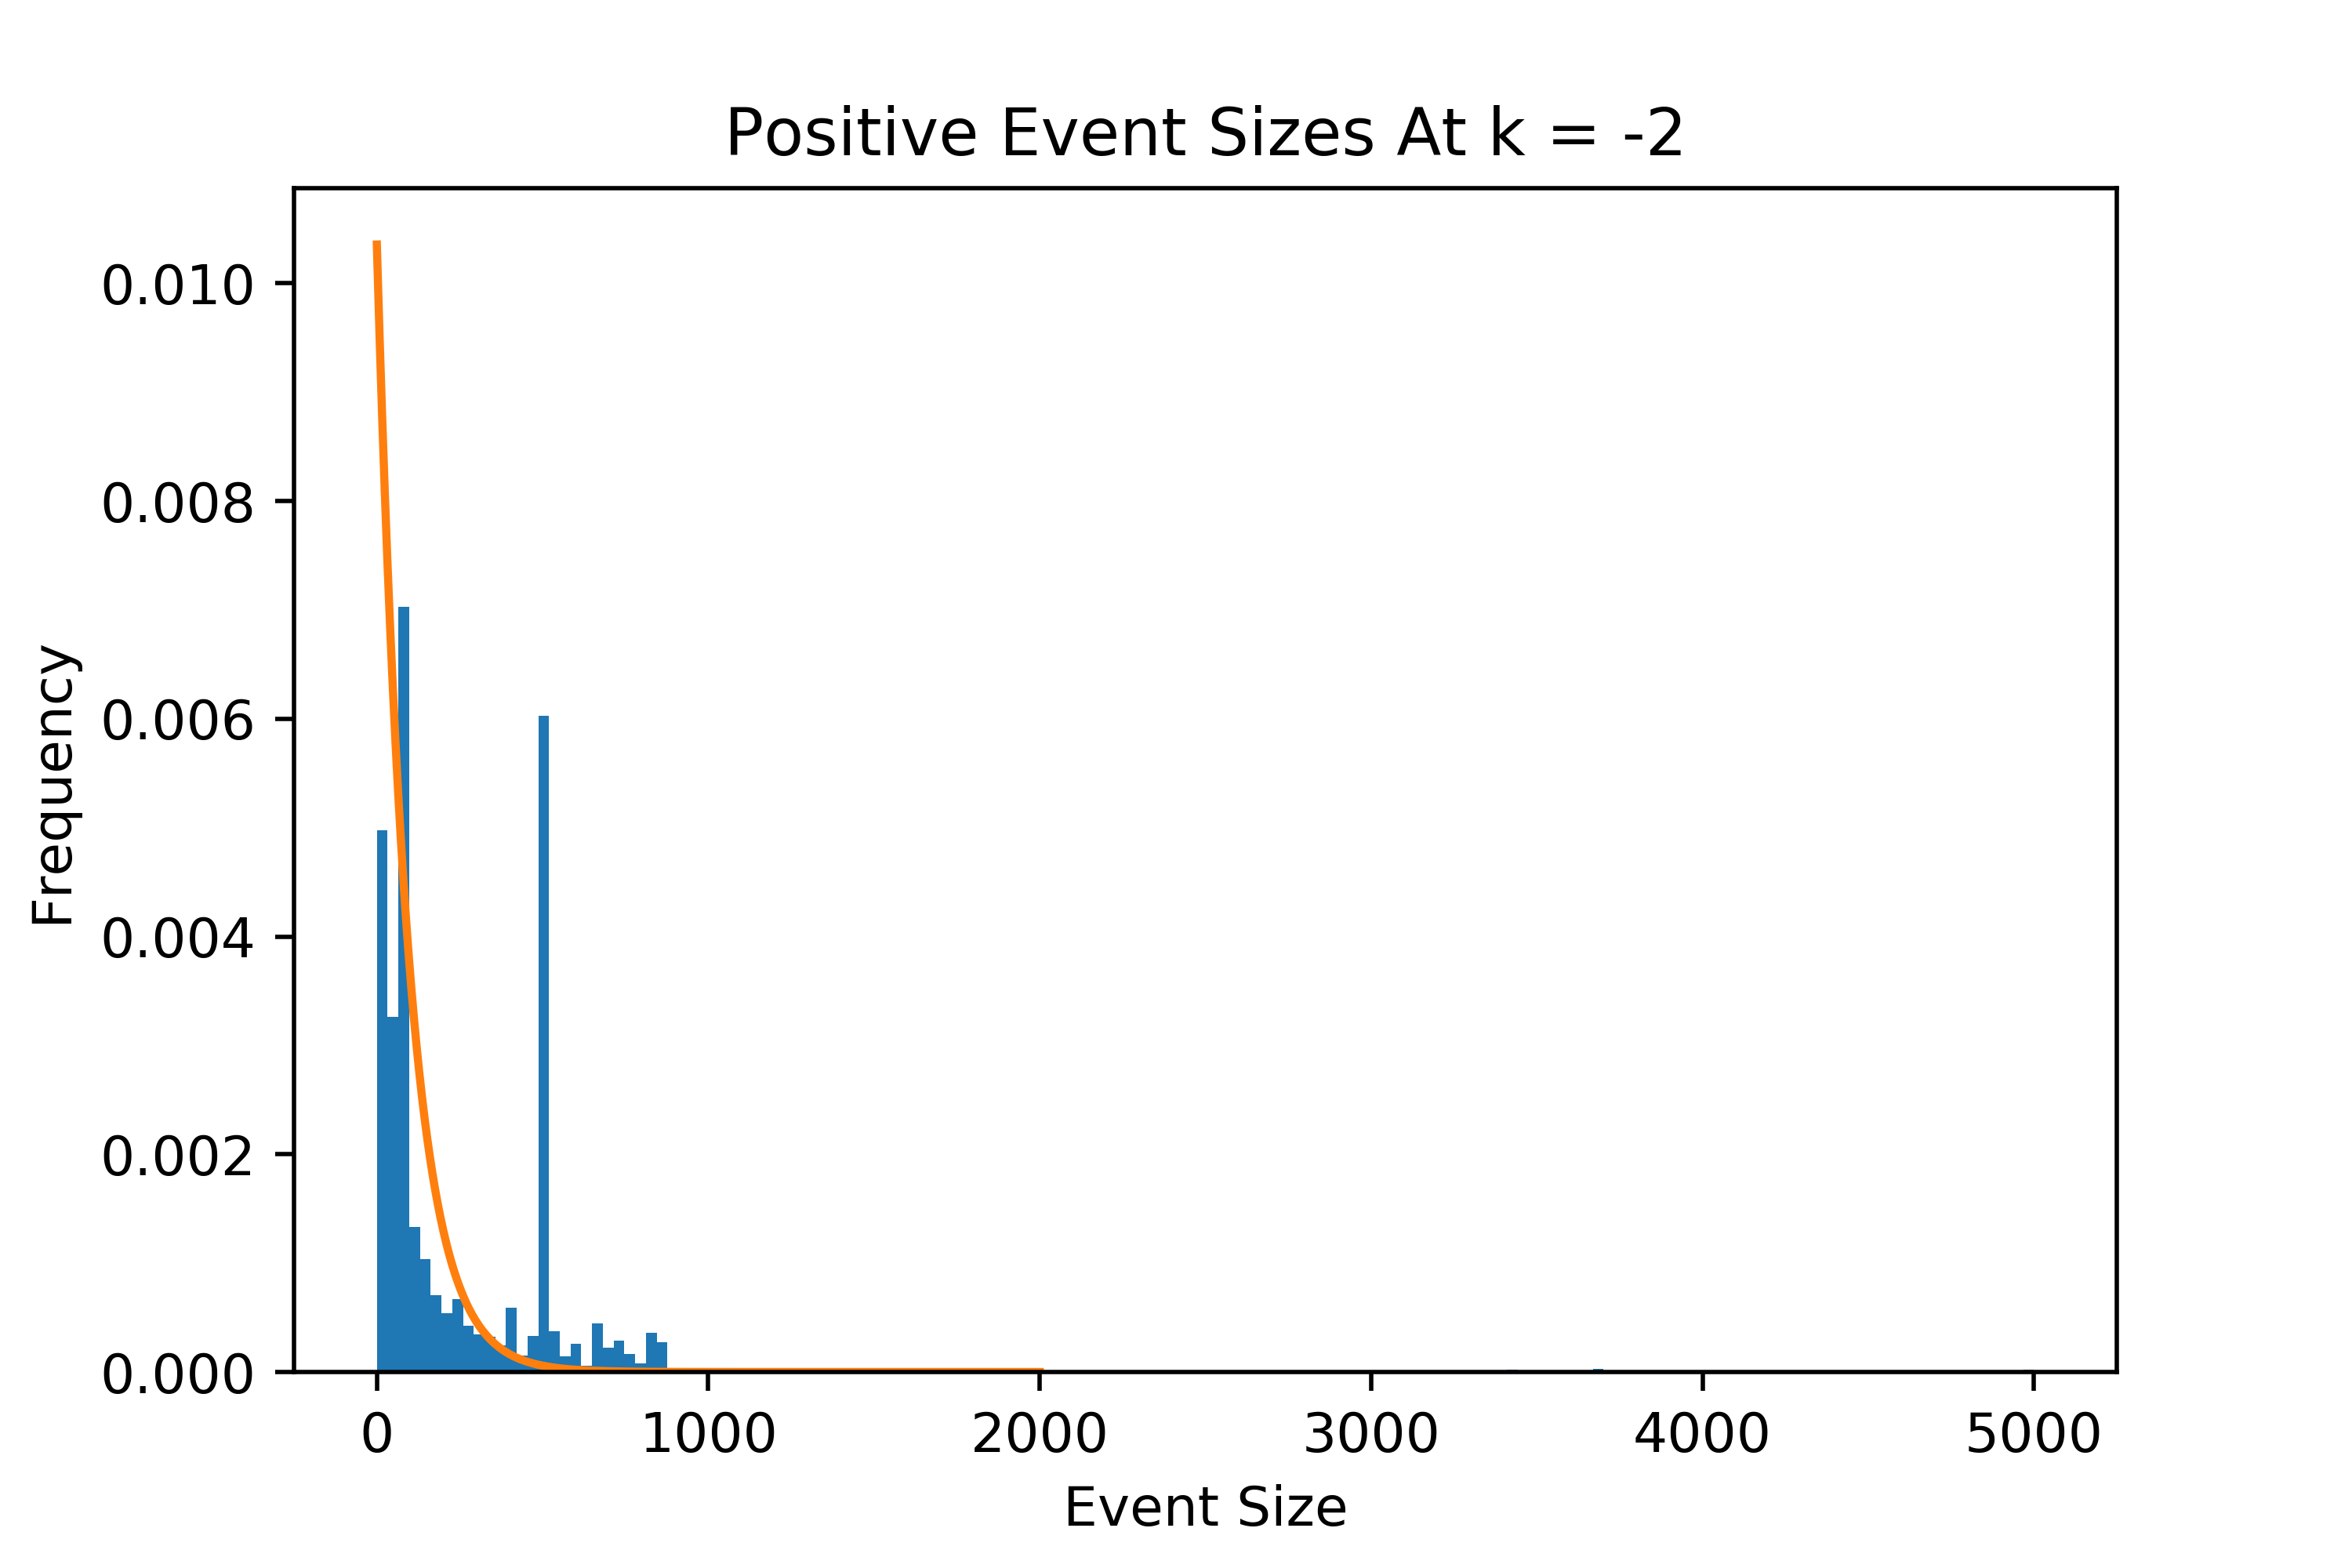
\includegraphics[width=60mm]{Figures/pos_-2.png}}
{}
&
\subf{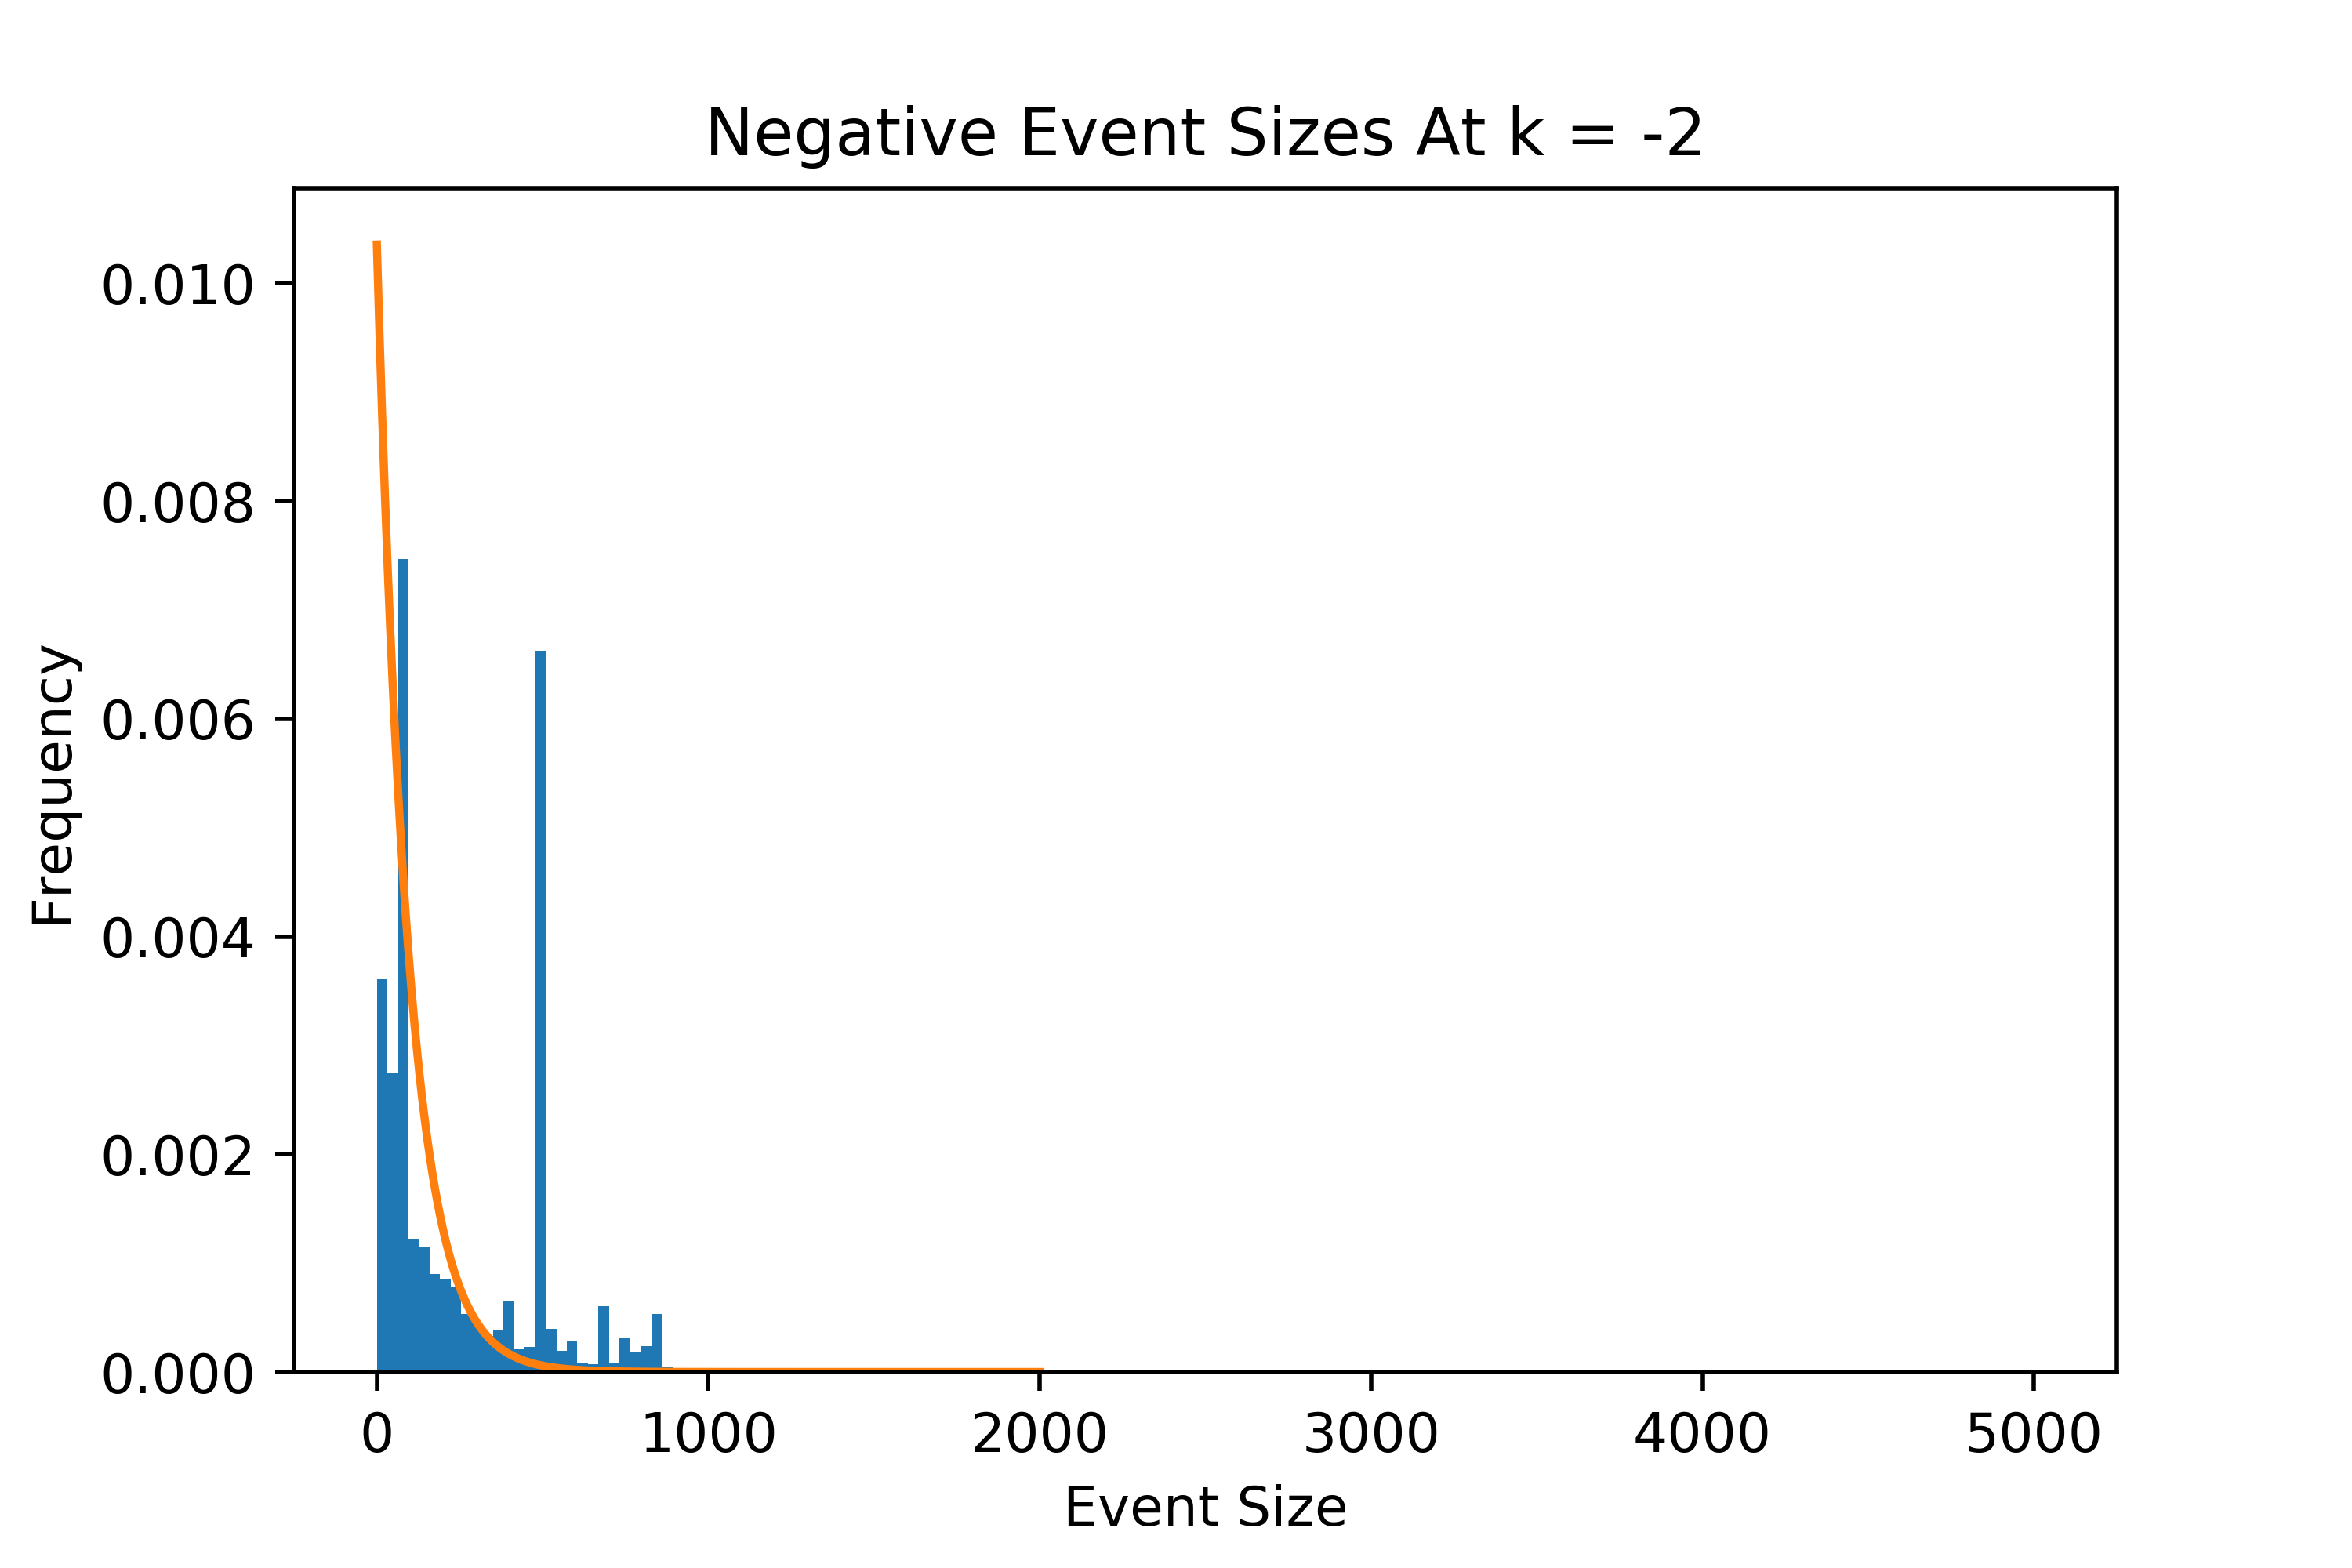
\includegraphics[width=60mm]{Figures/neg_-2.png}}
{}
\\
\subf{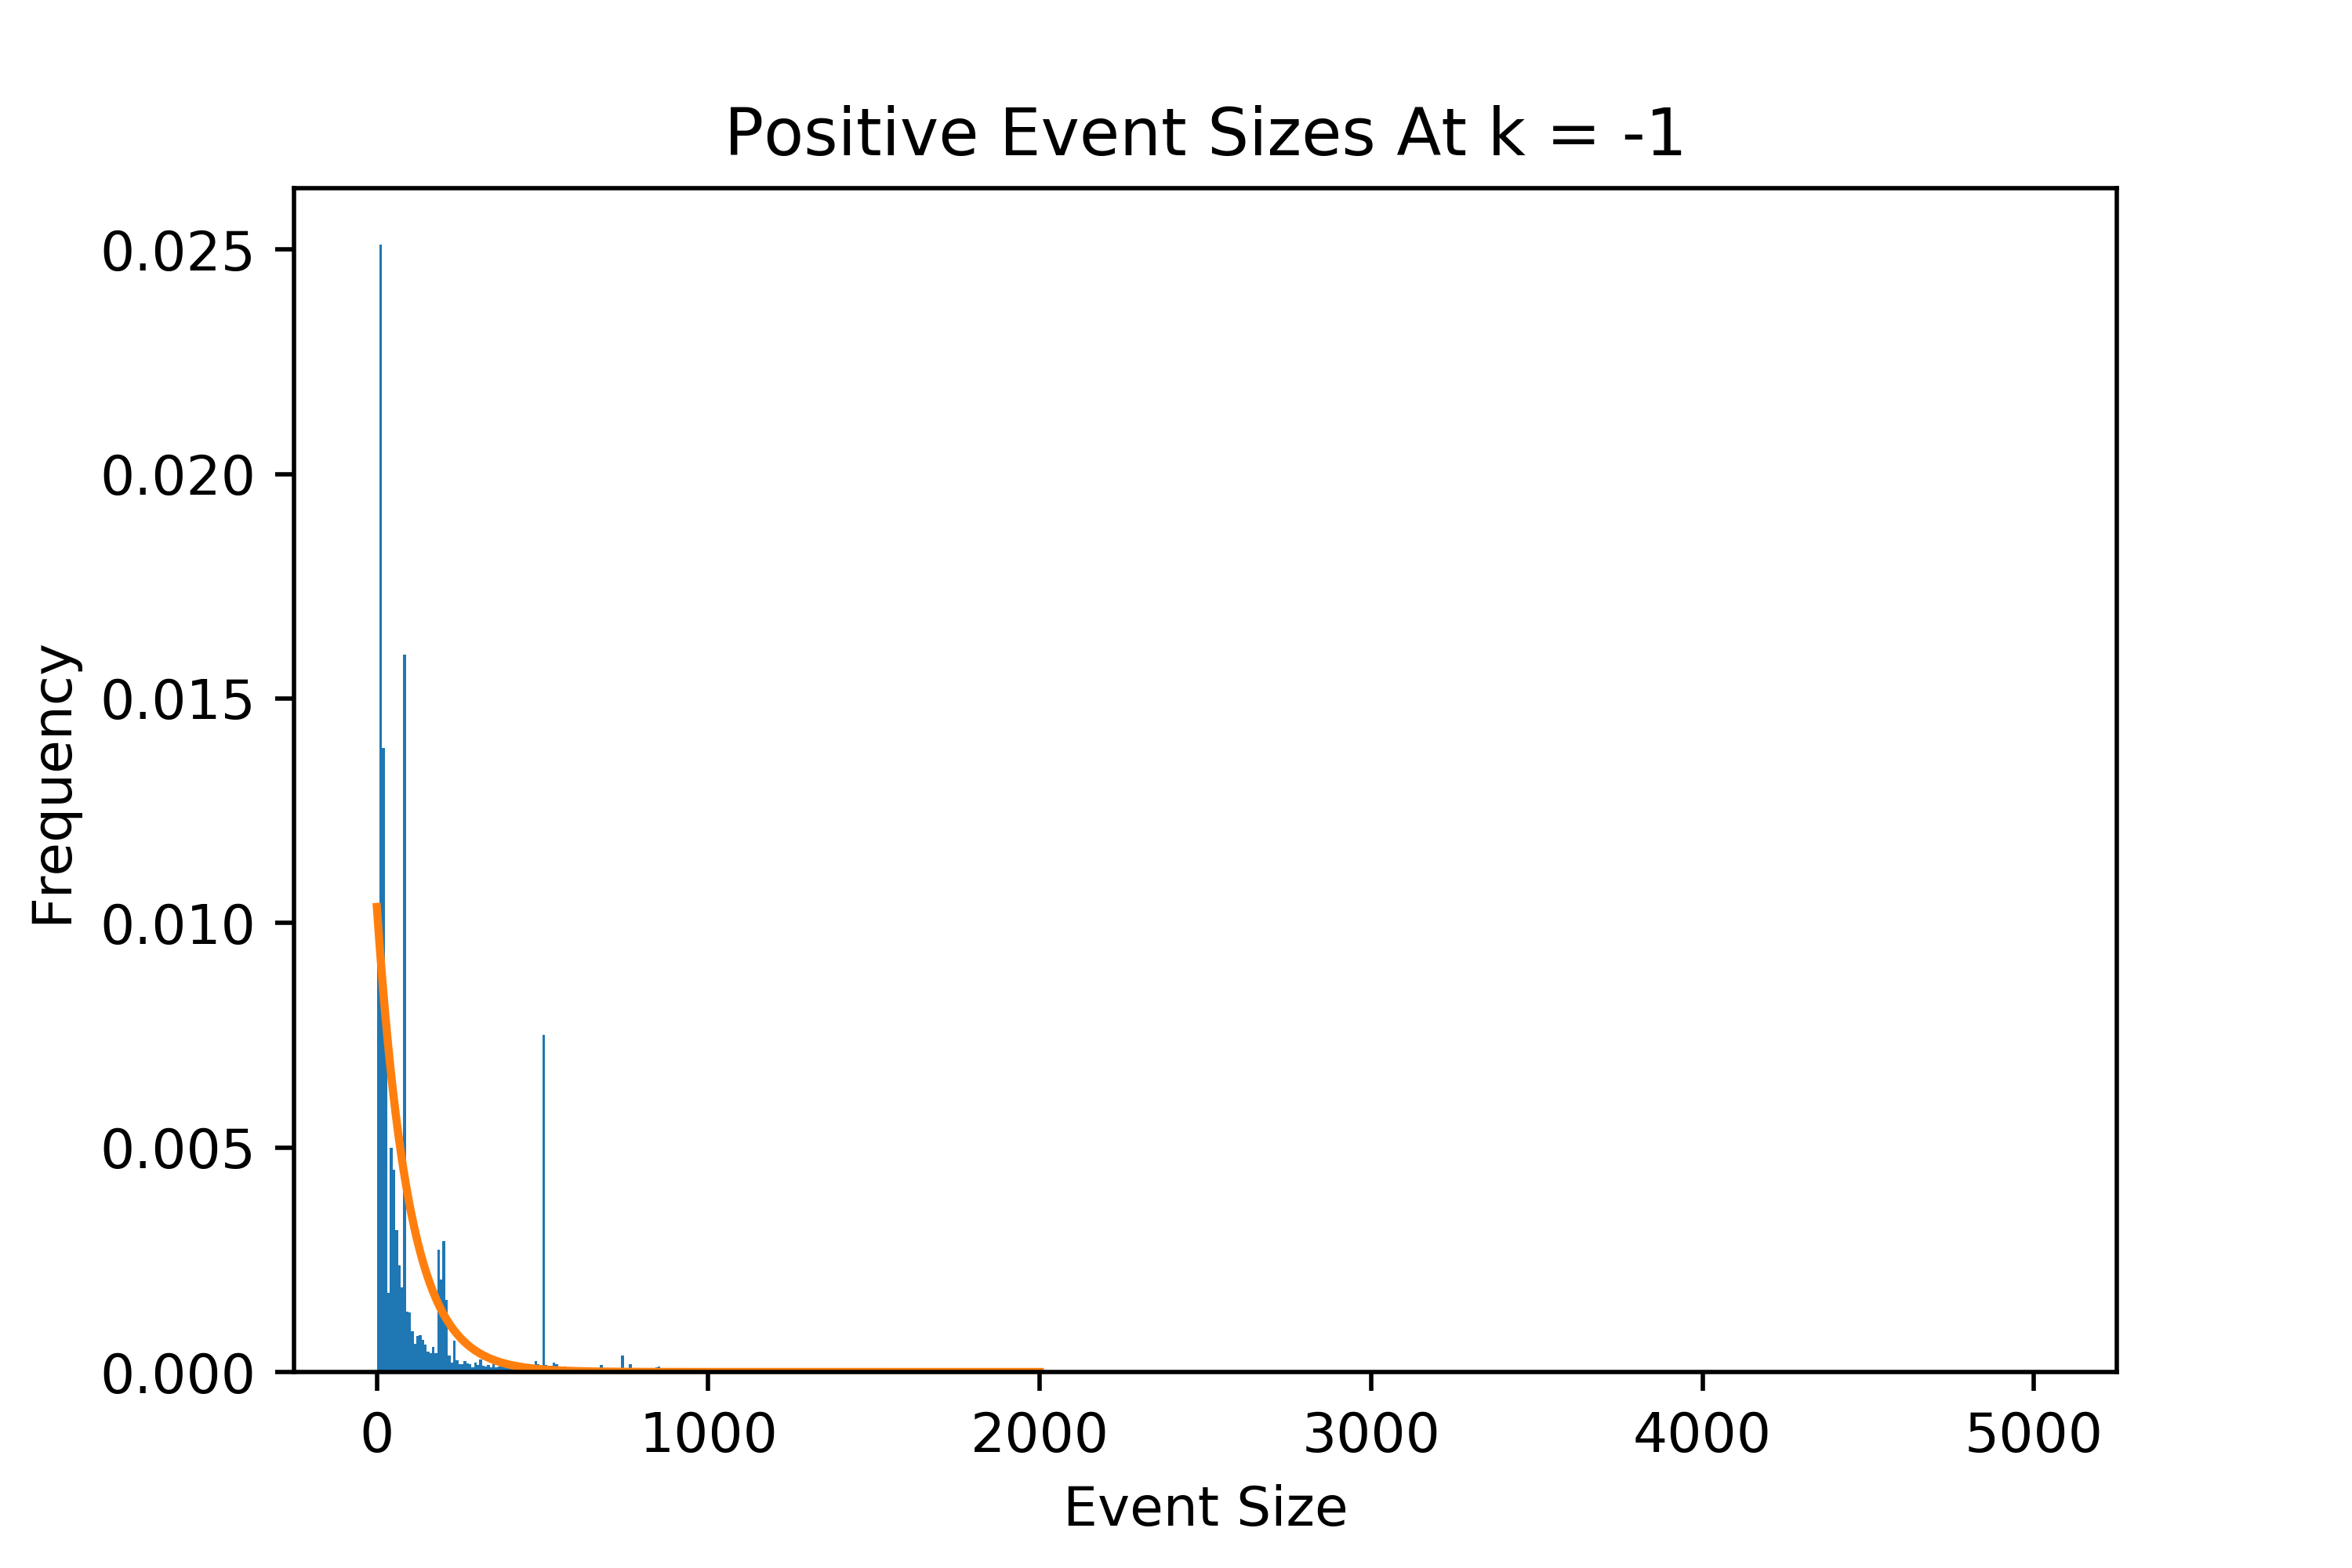
\includegraphics[width=60mm]{Figures/pos_-1.png}}
{}
&
\subf{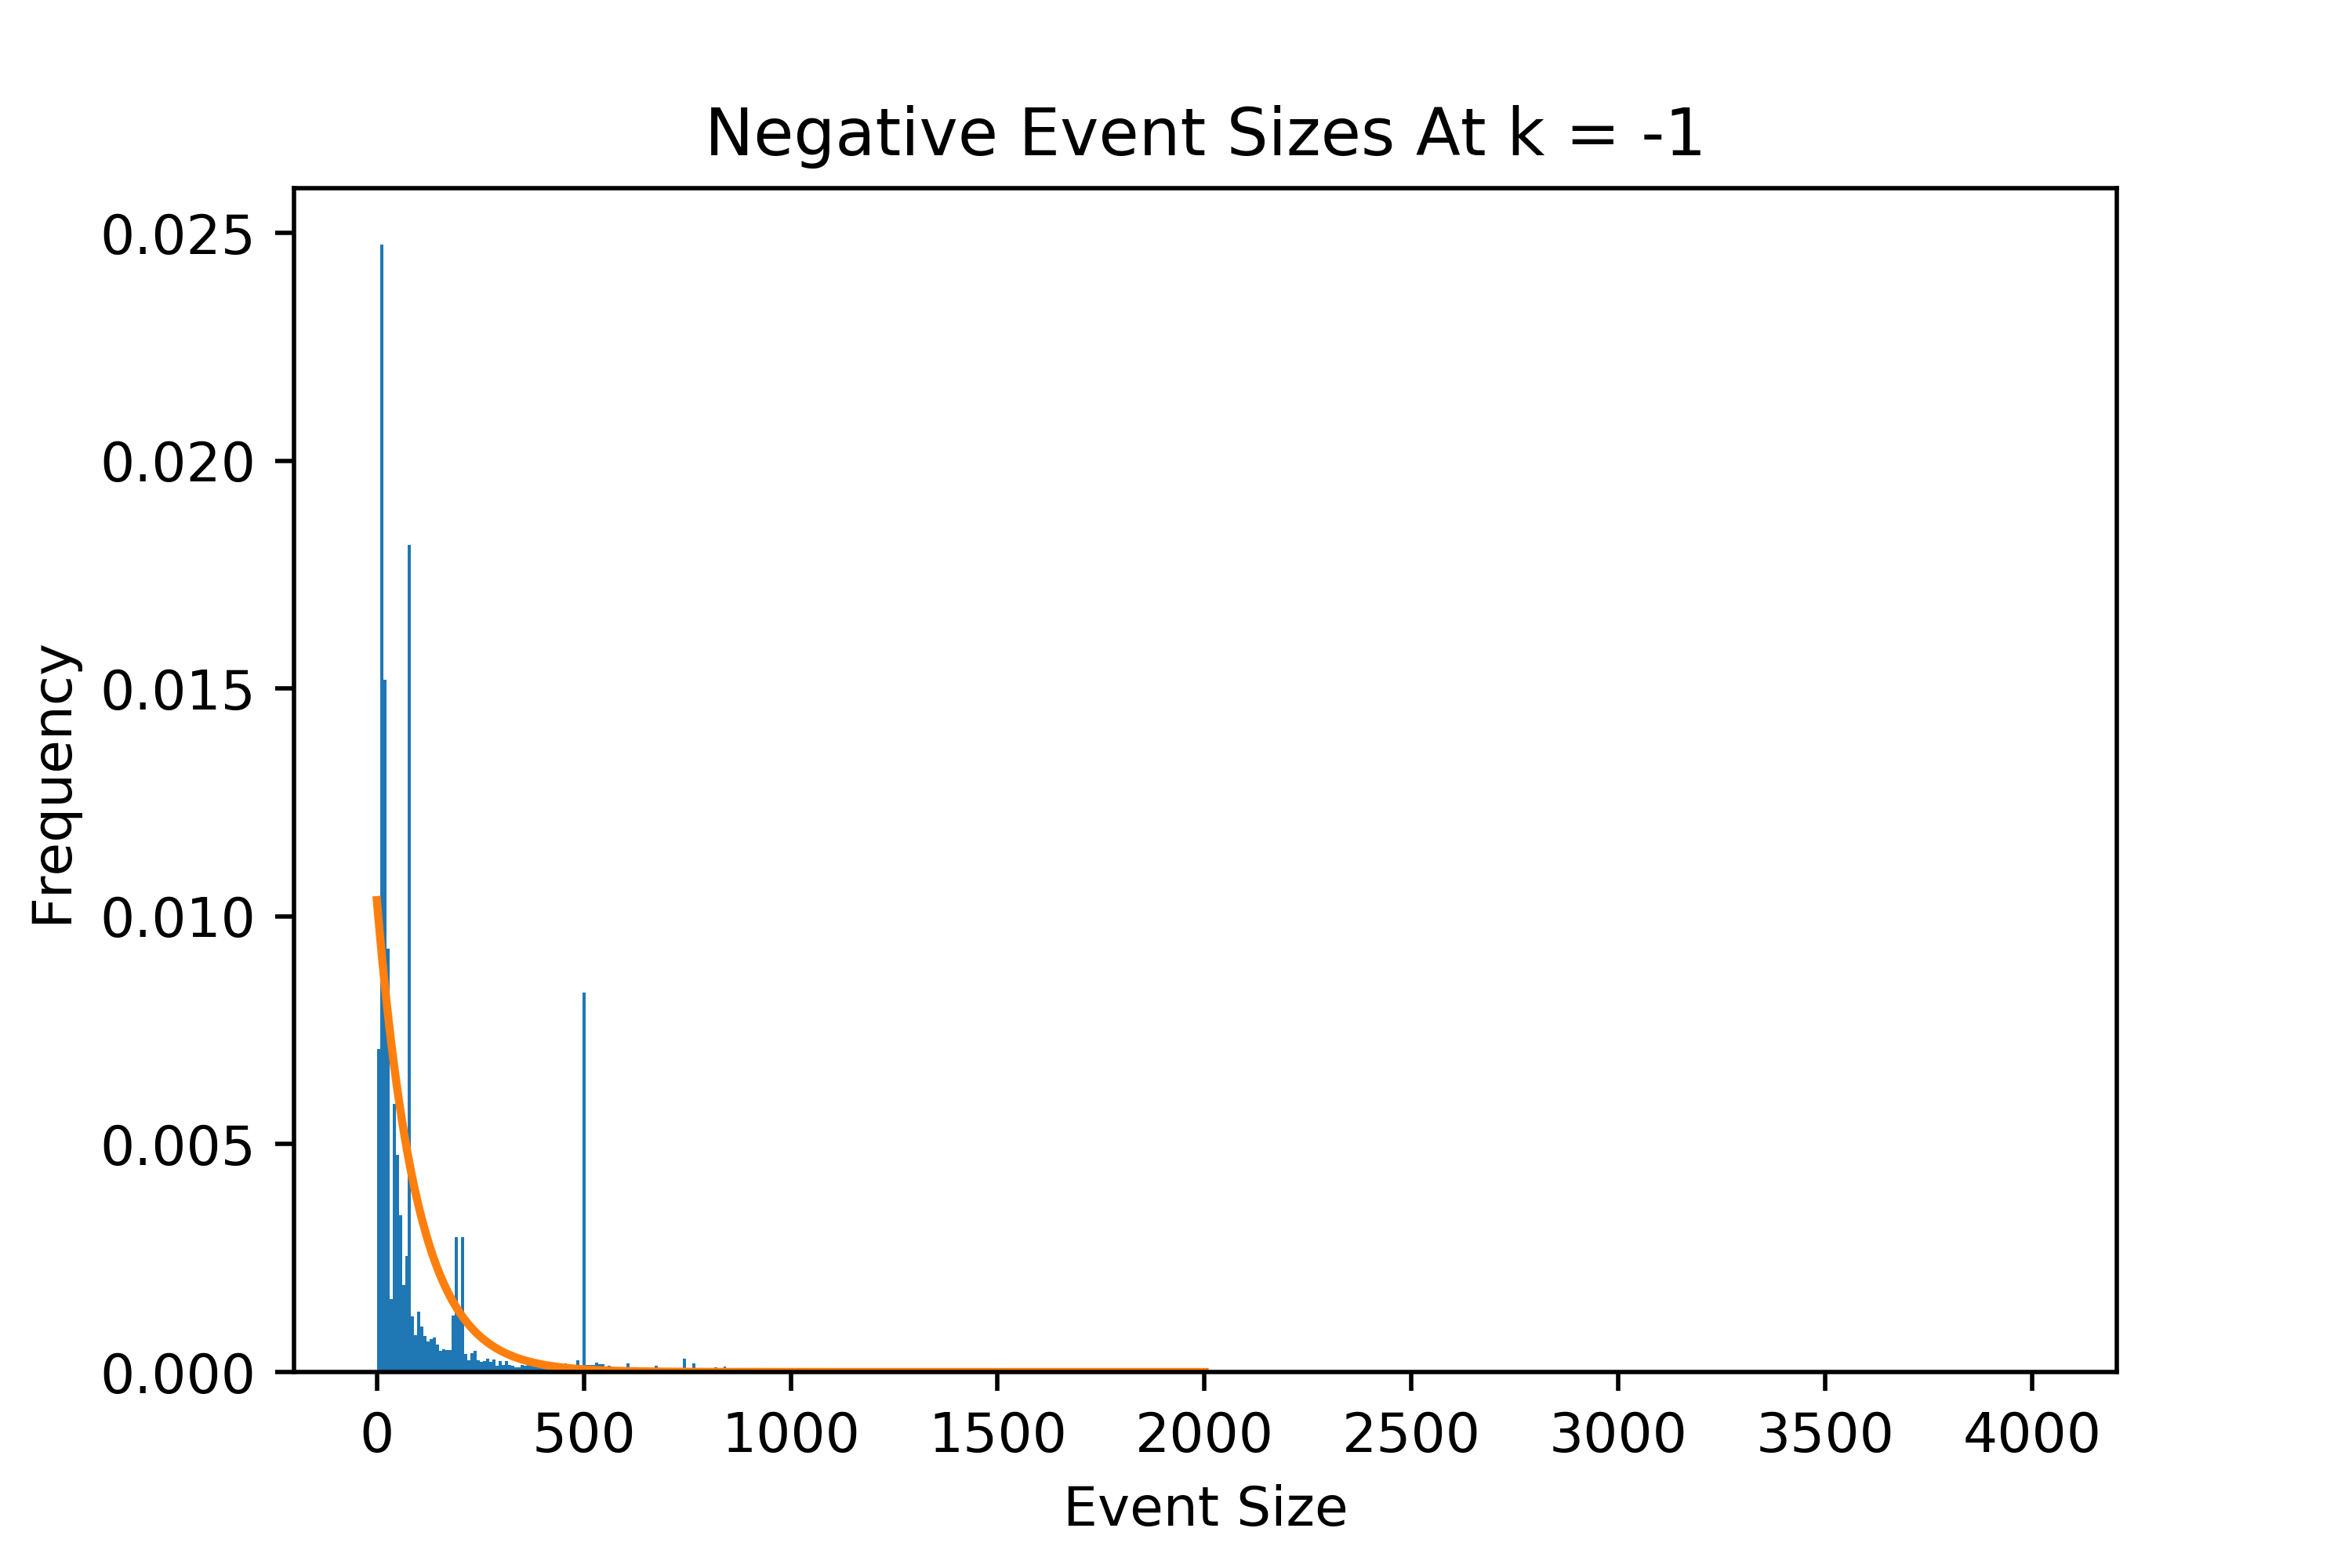
\includegraphics[width=60mm]{Figures/neg_-1.png}}
{}
\\
\subf{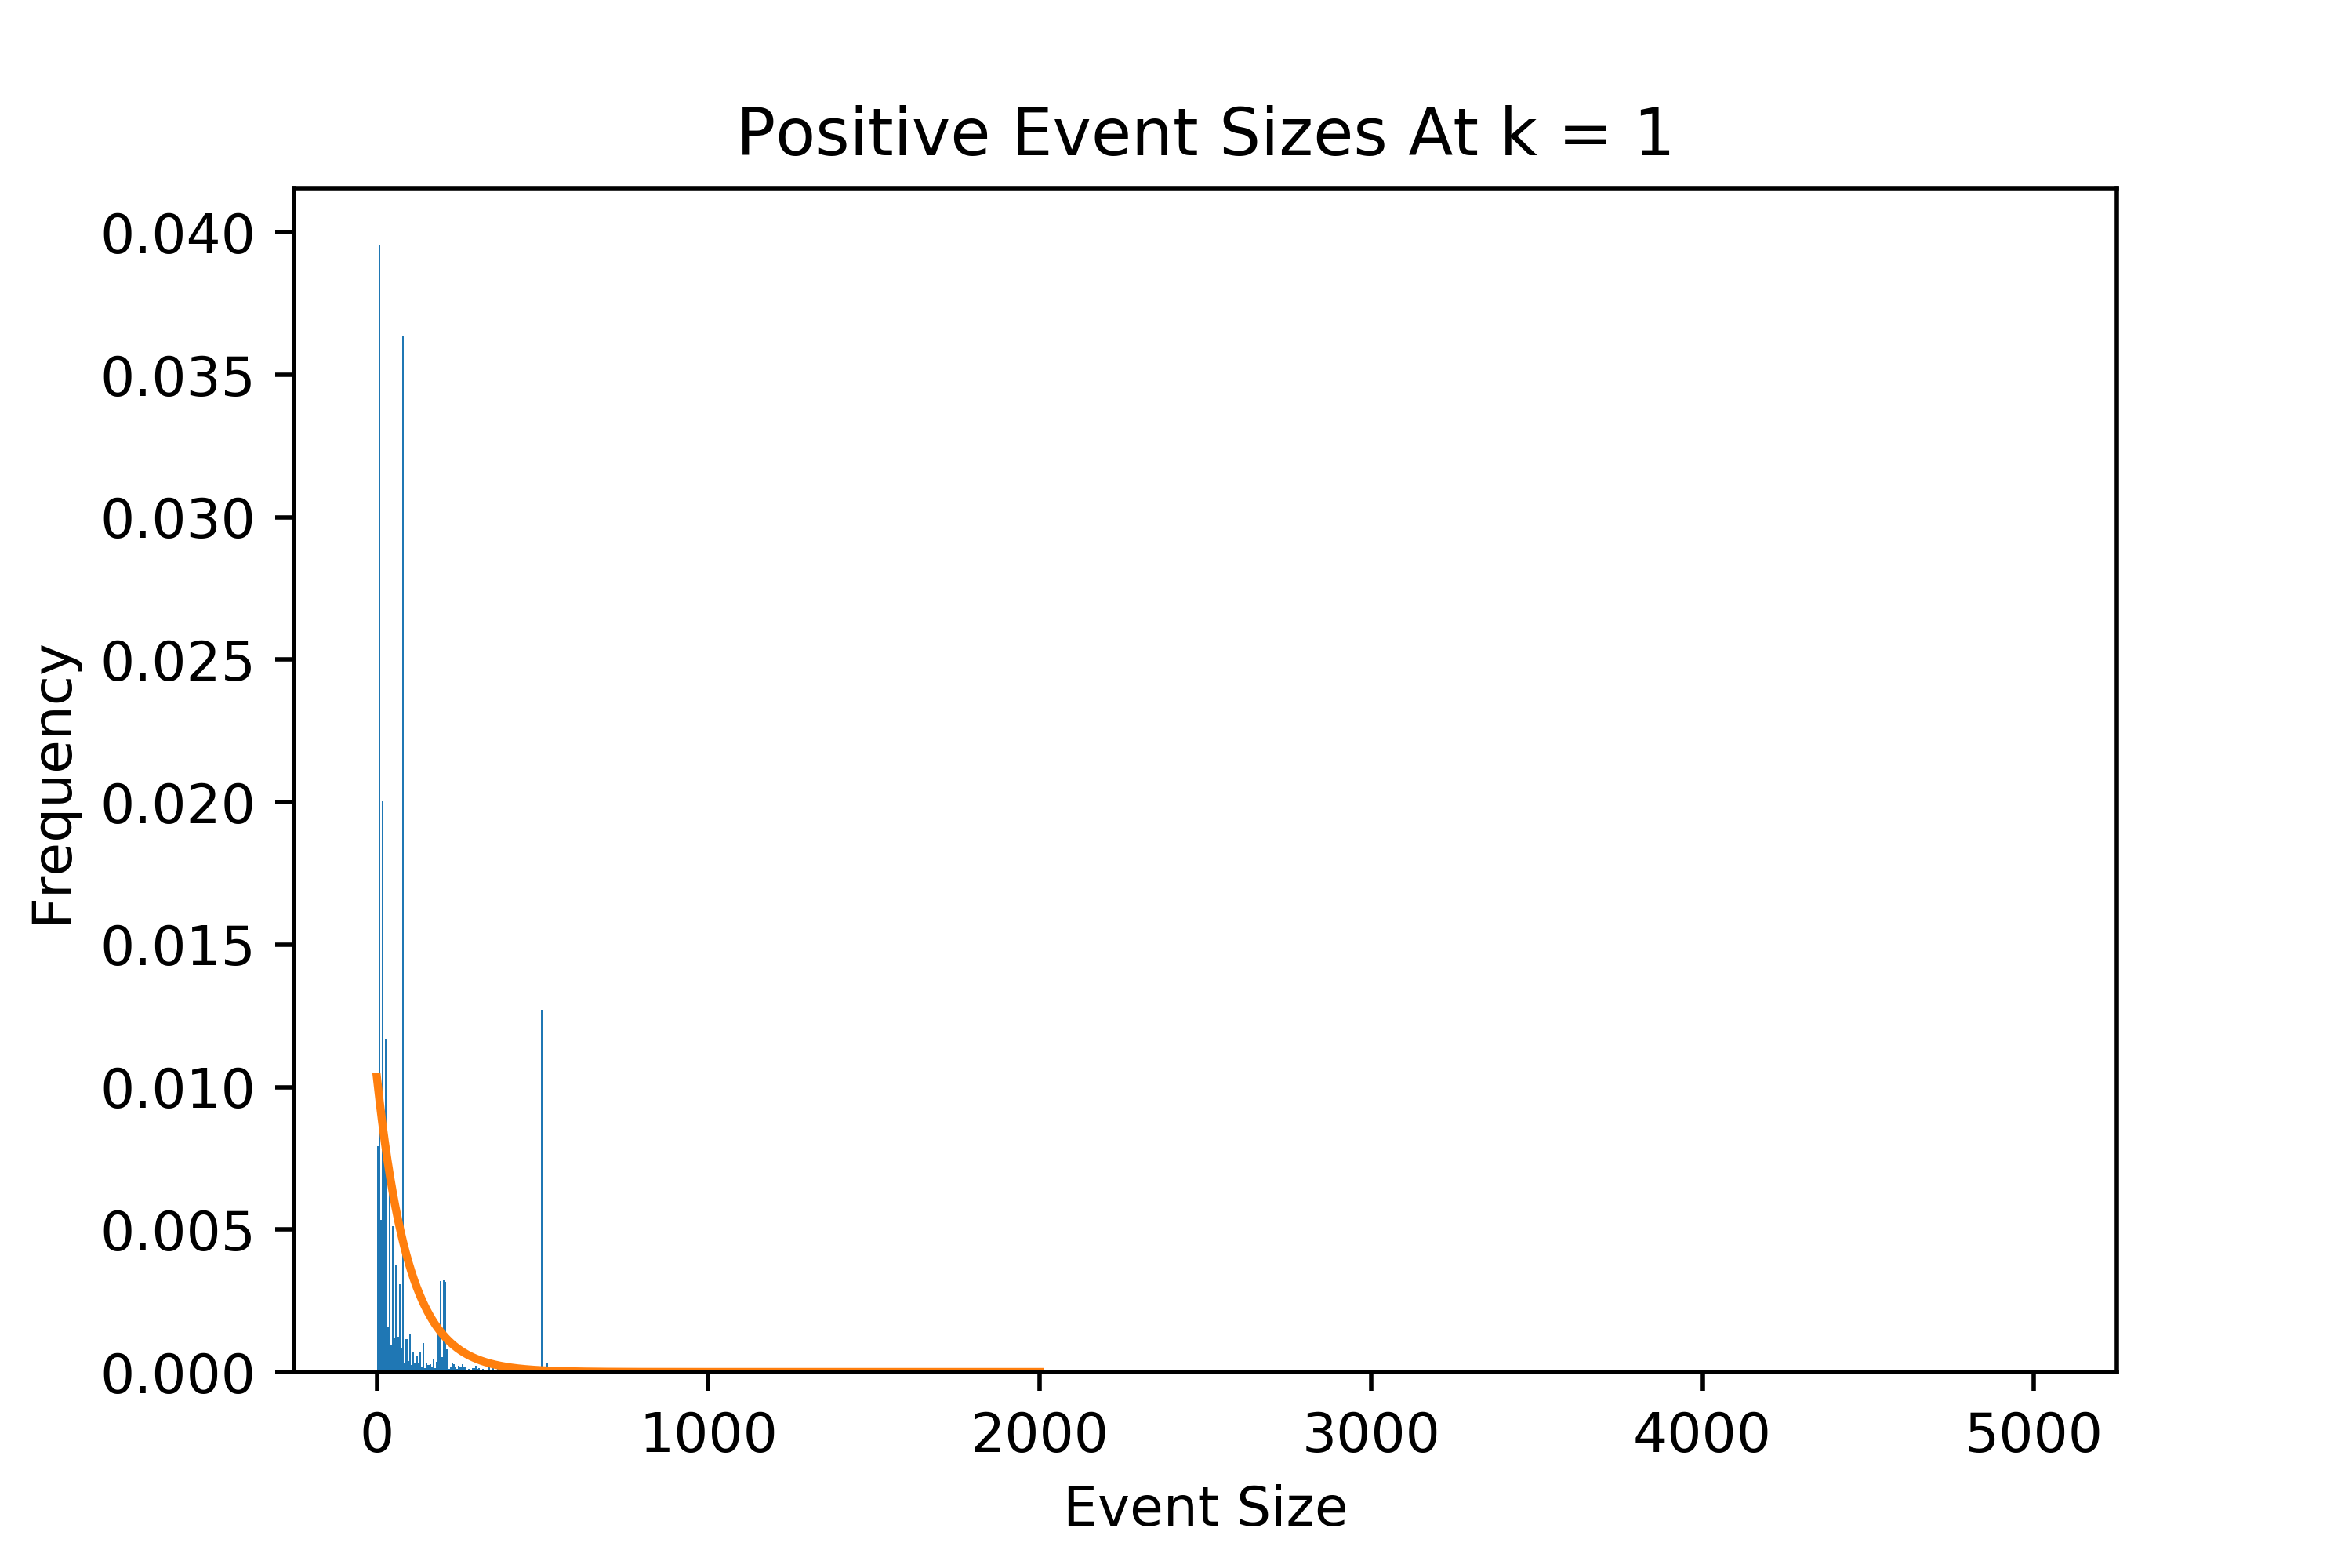
\includegraphics[width=60mm]{Figures/pos_1.png}}
{}
&
\subf{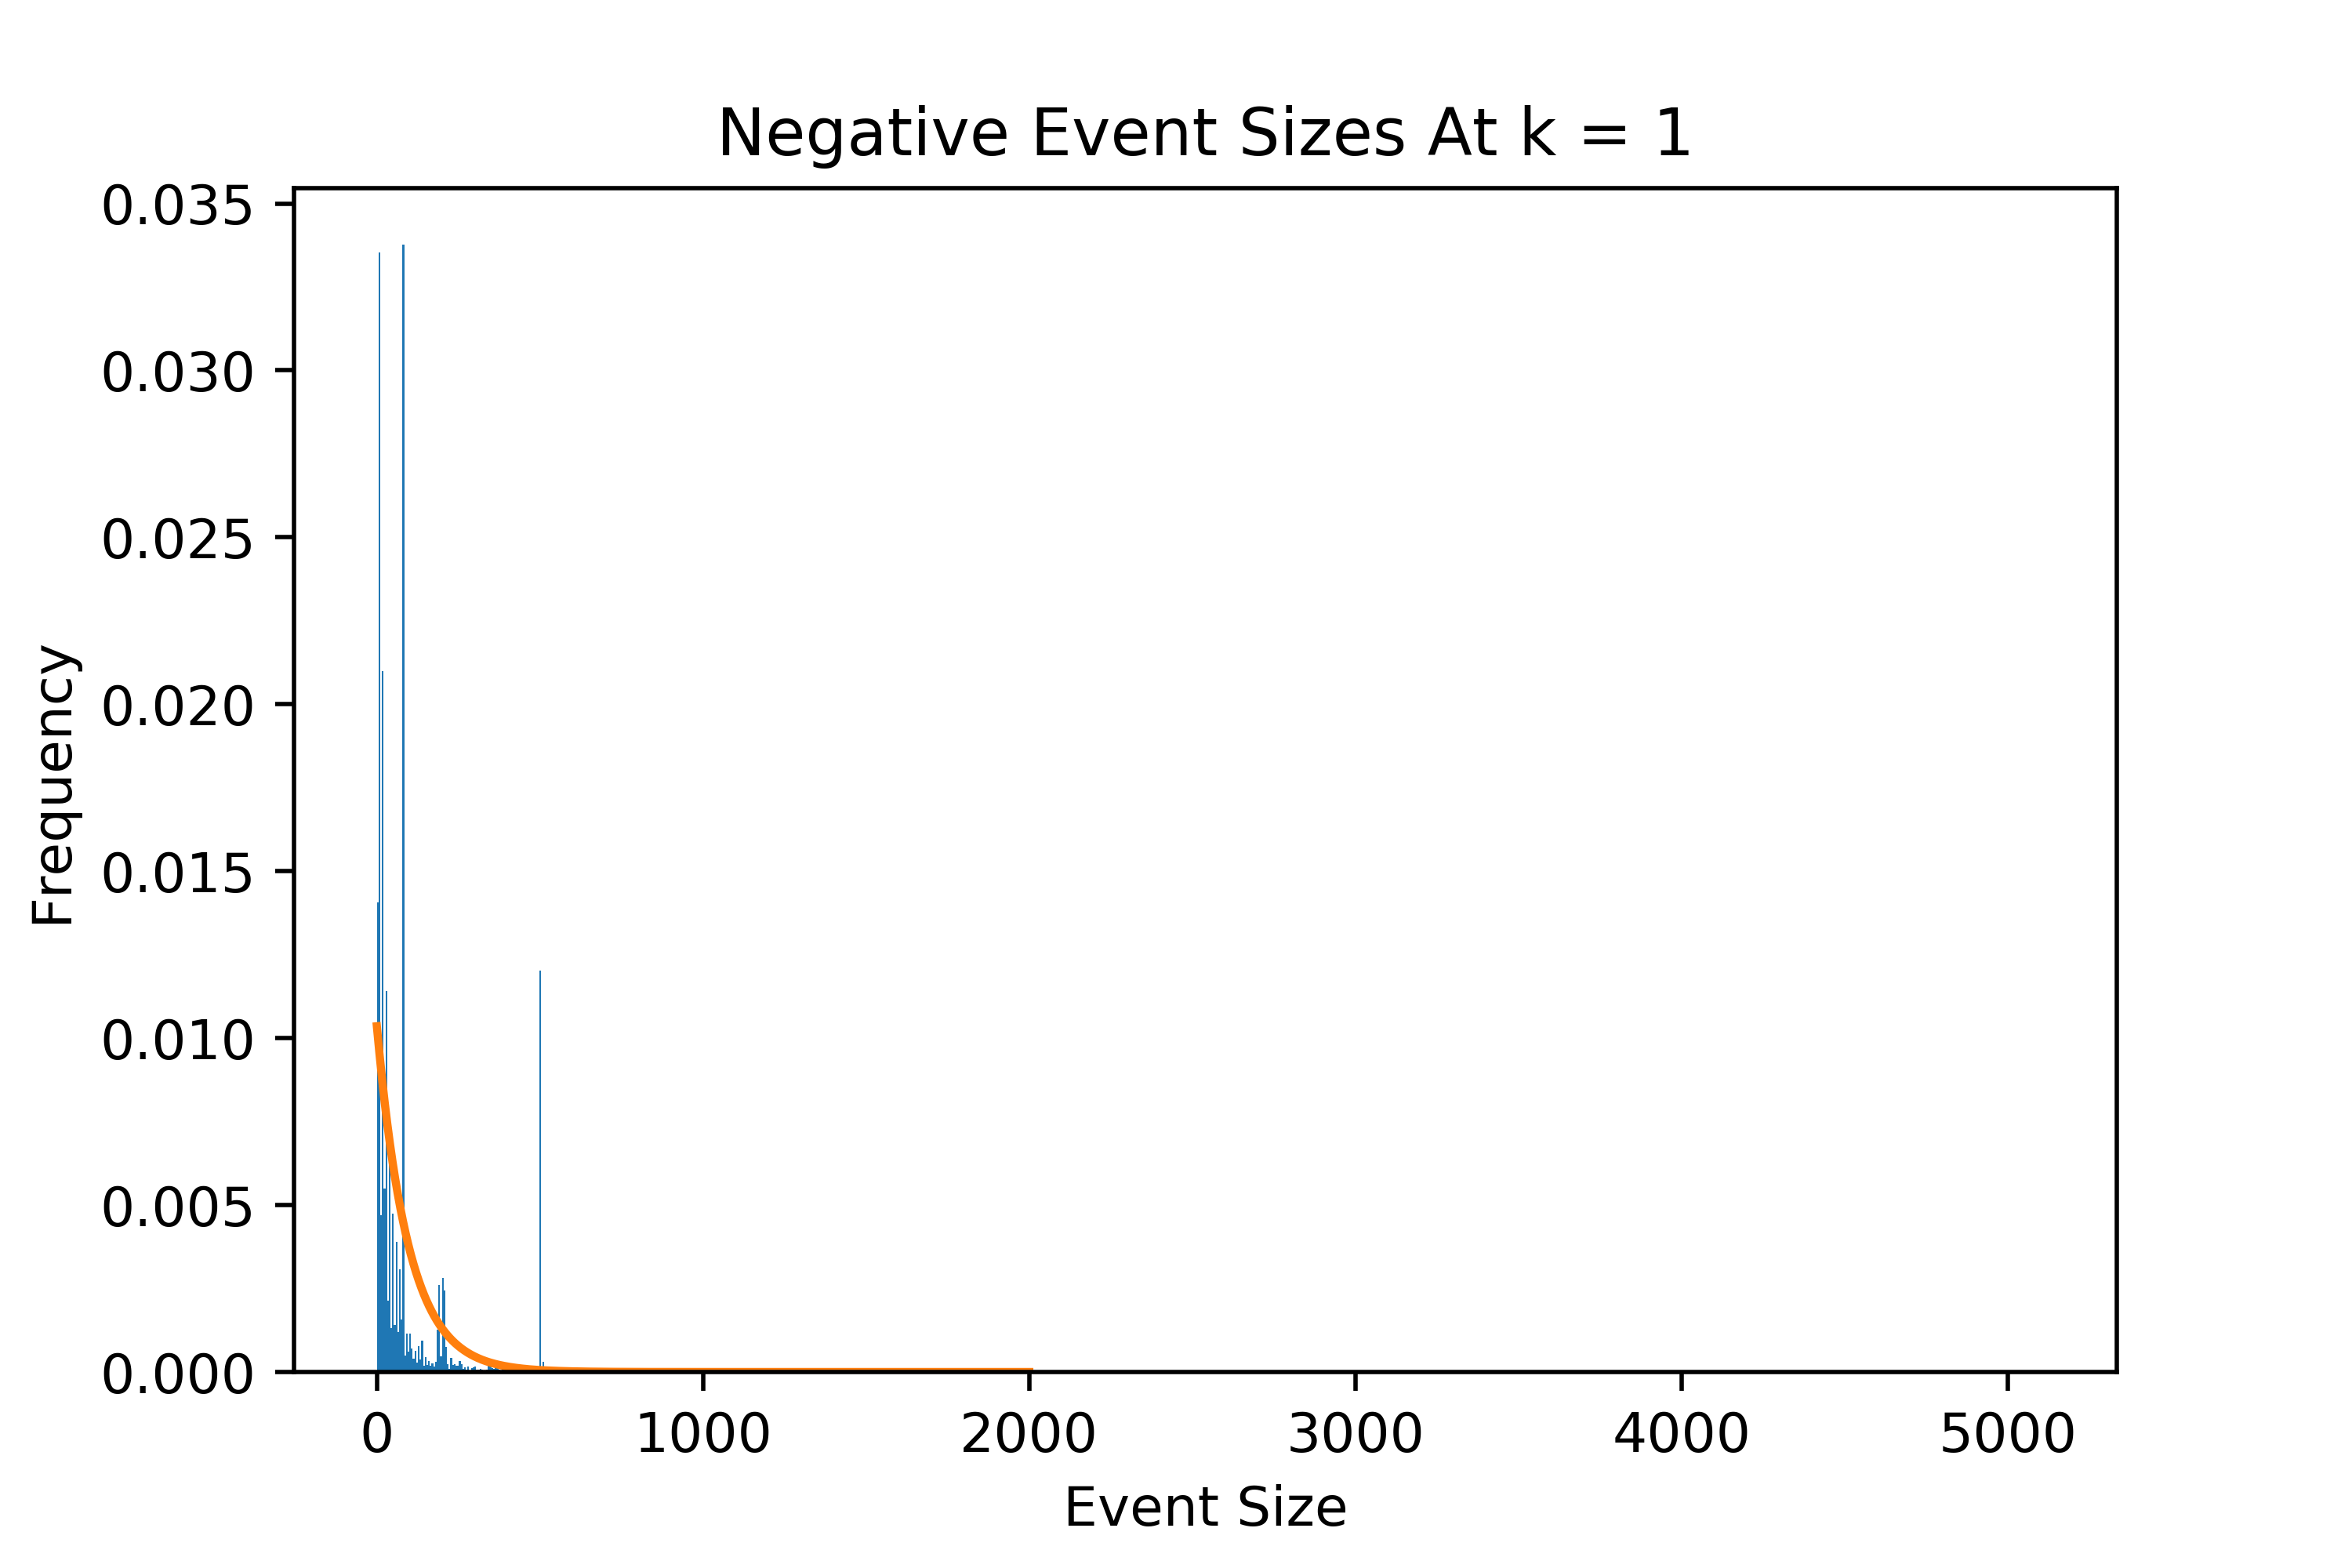
\includegraphics[width=60mm]{Figures/neg_1.png}}
{}
\\
\subf{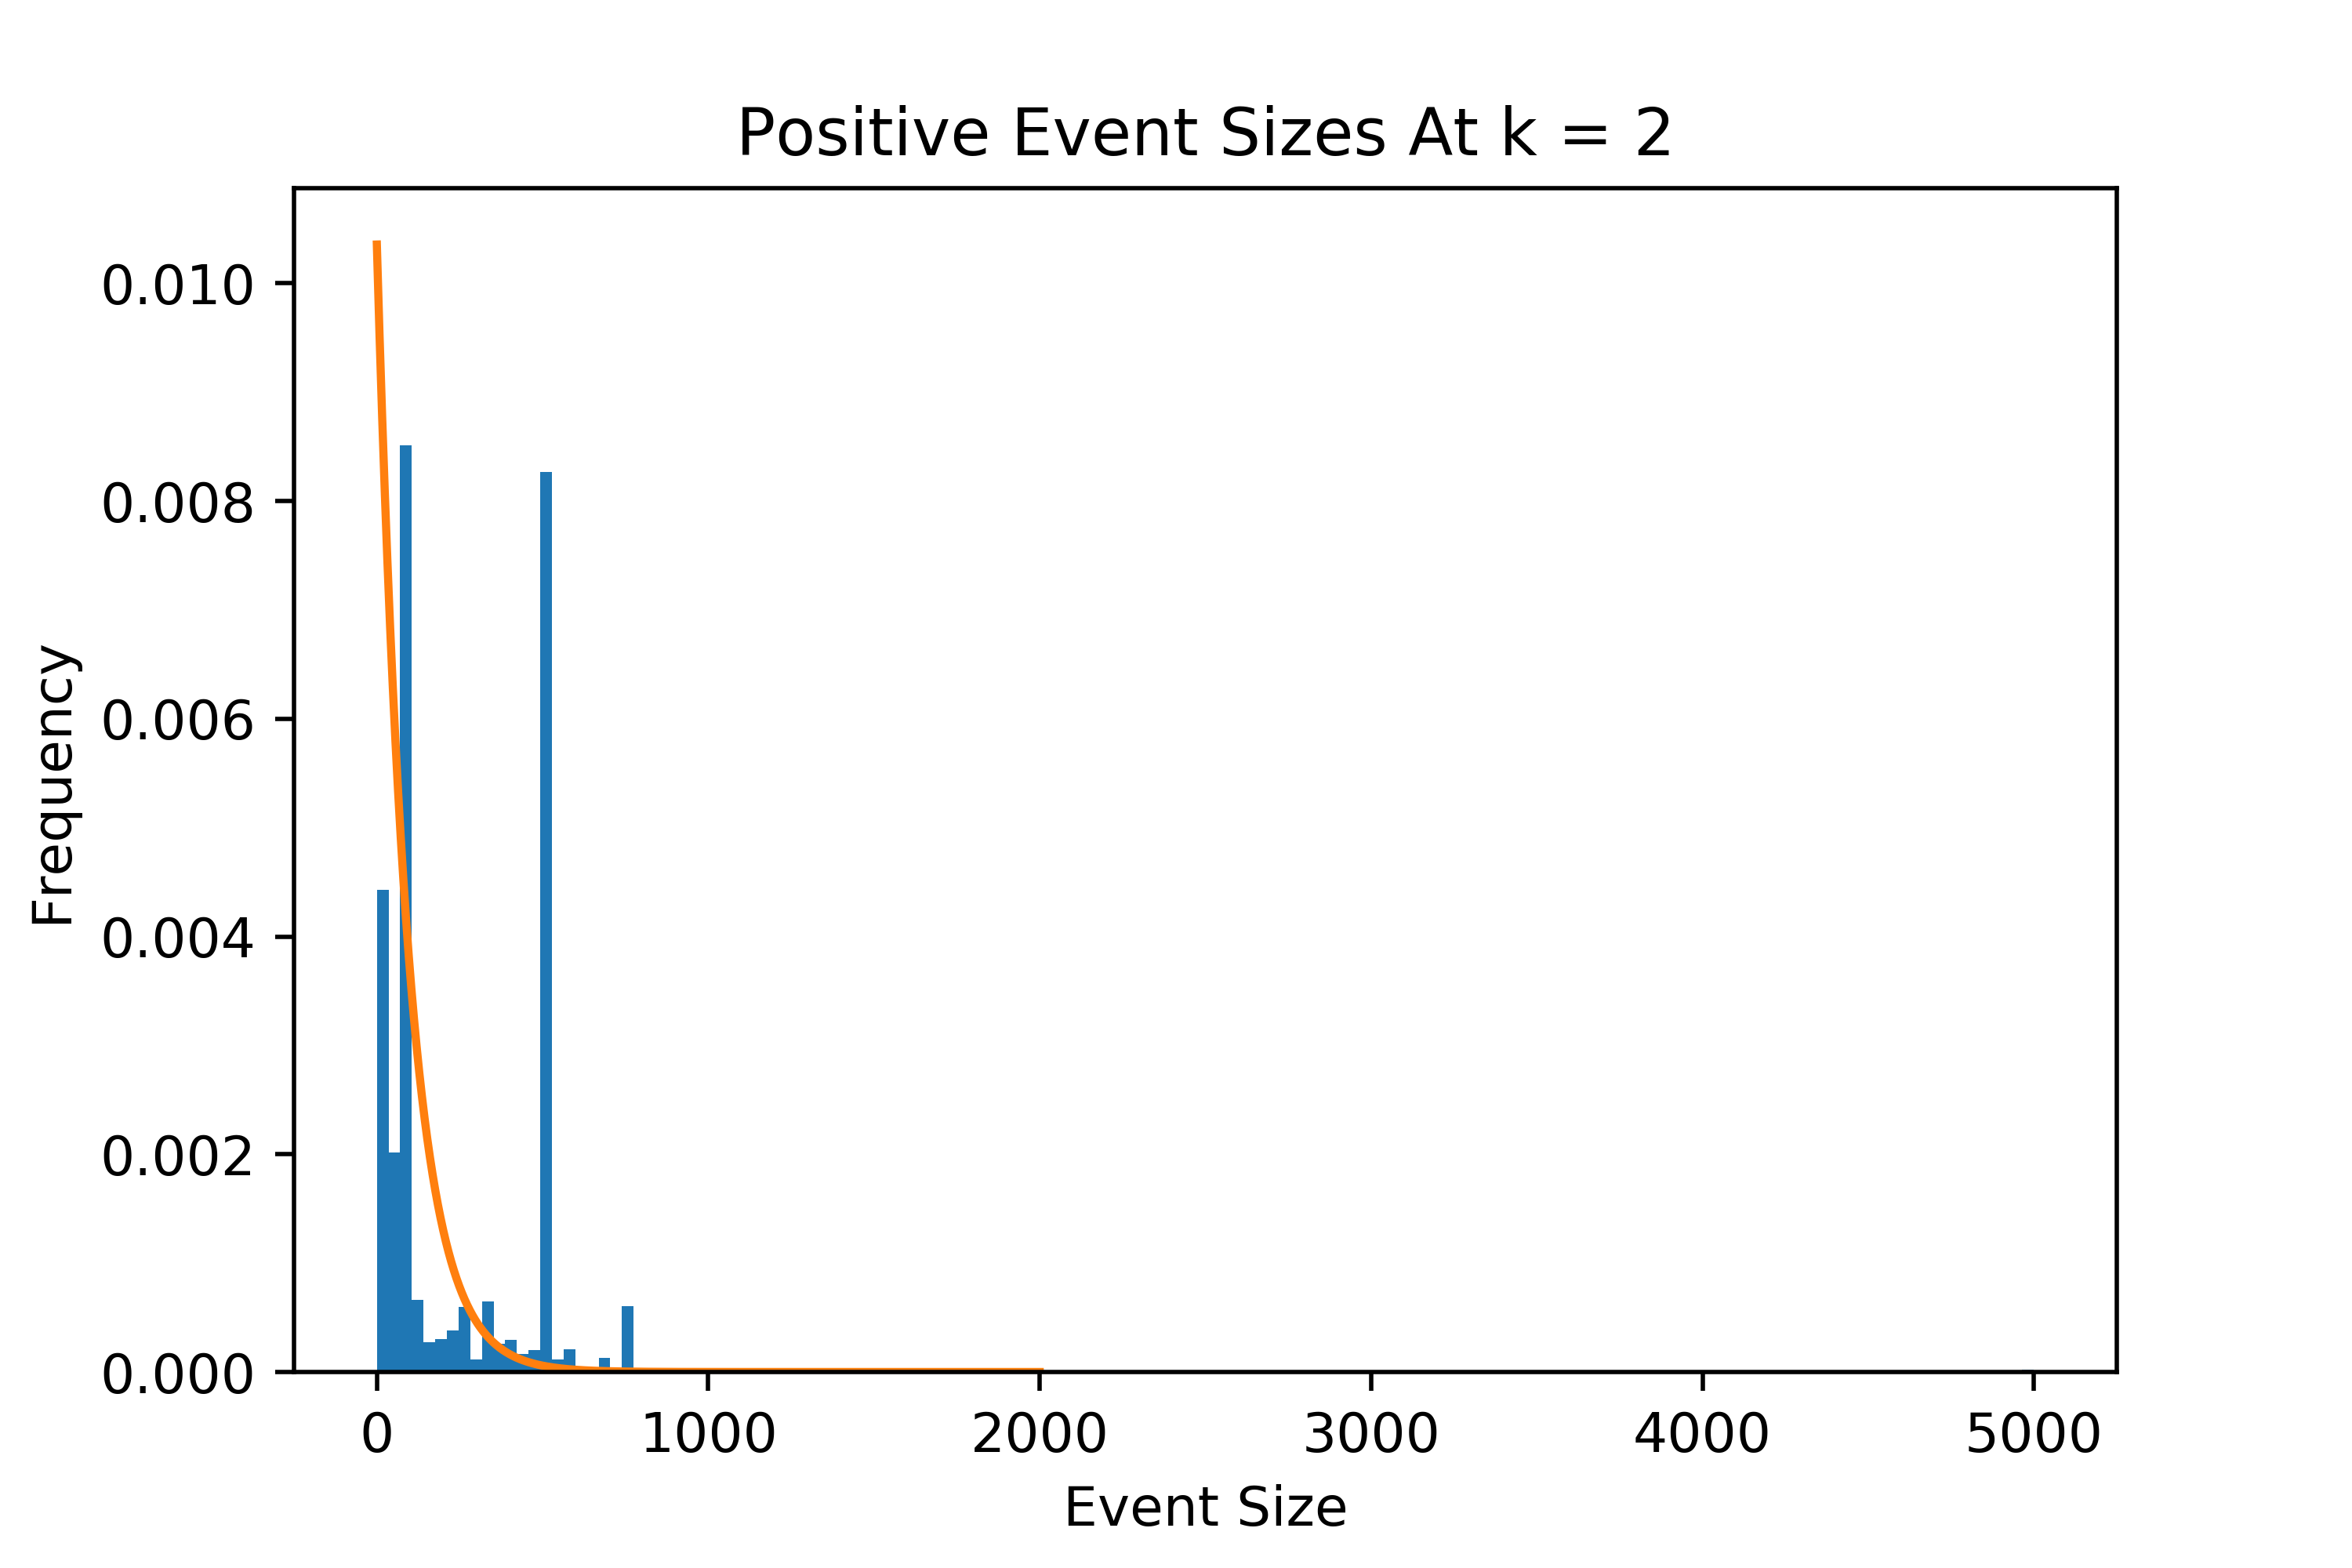
\includegraphics[width=60mm]{Figures/pos_2.png}}
{}
&
\subf{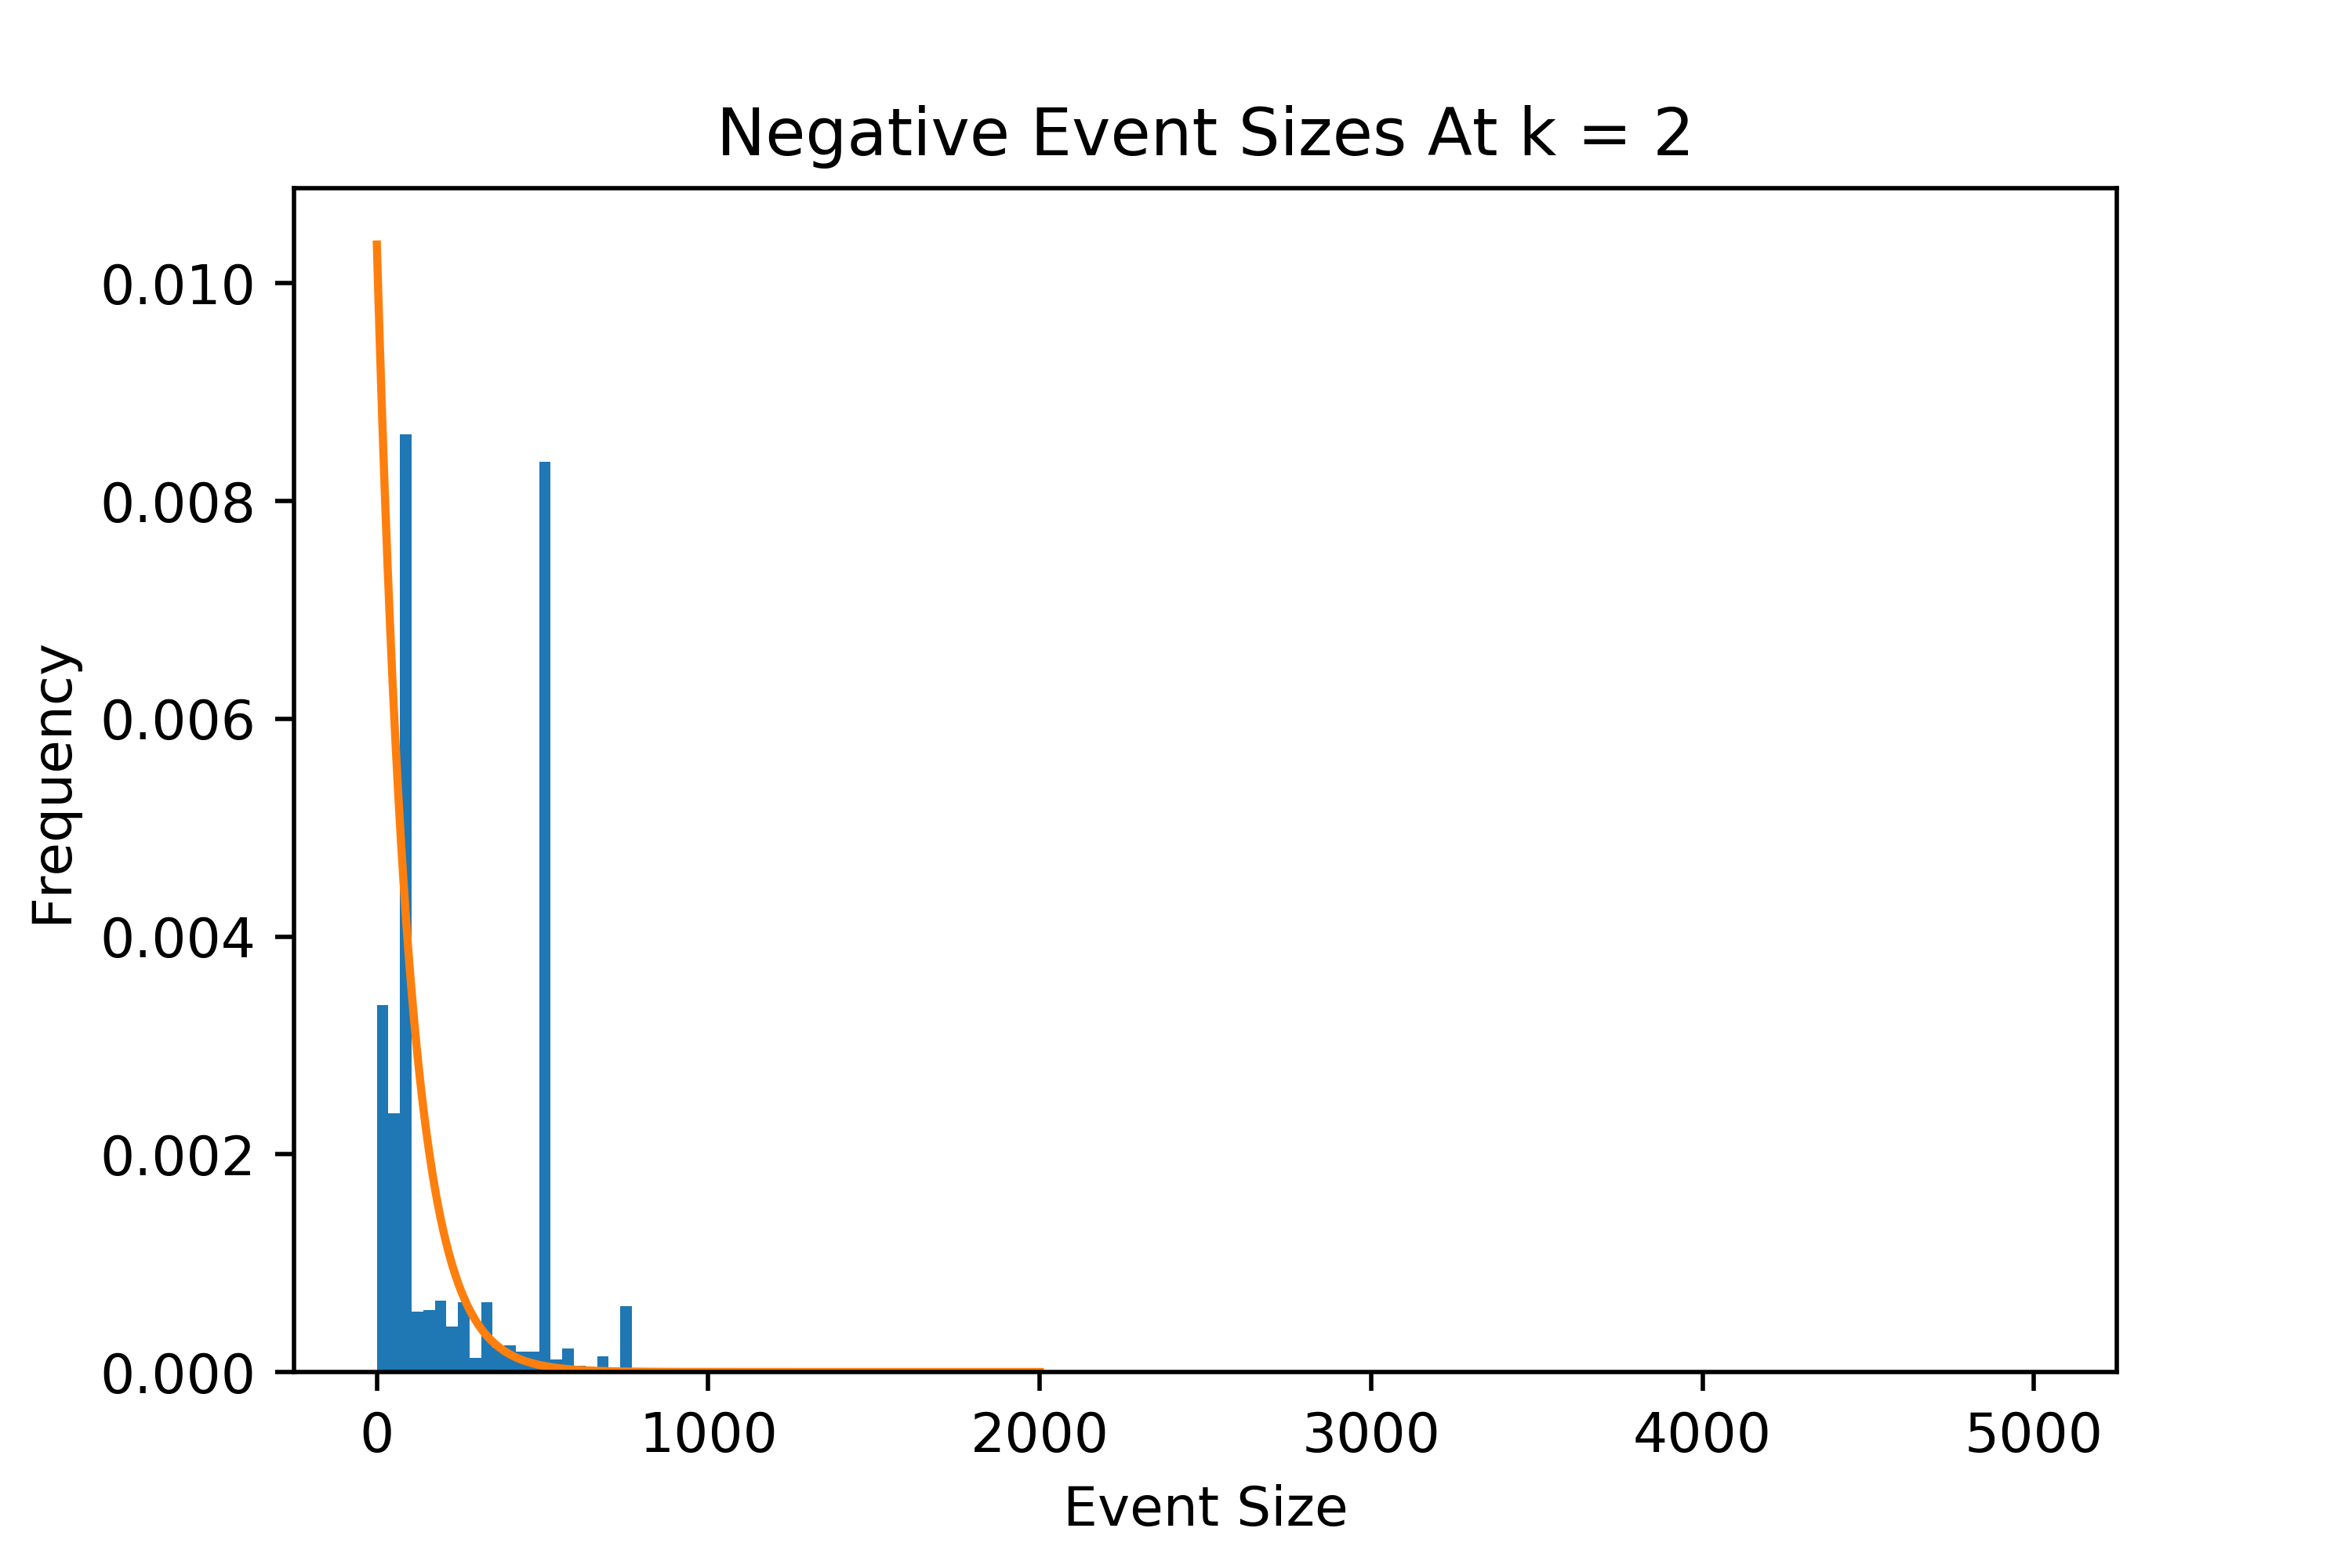
\includegraphics[width=60mm]{Figures/neg_2.png}}
{}
\\
\hline
\end{tabular}
\label{fig:sizes}
\end{figure}

Histograms of event sizes at each position are shown in Figure \ref{fig:sizes}. Exponential distributions with means equal to the $AES$'s are overlaid on top. As can be seen, the exponential distributions fit the histograms relatively well. However, there are some notable discrepancies. One is the high frequency of orders at 500. A possible explanation for this observation is that 500 may be a common size used by traders to split up large orders. There are also a non-negligible number of orders near 5000, since that is the upper limit order size imposed by Coinbase. Although it may be possible to more accurately model the dynamics of the ETC-USD LOB with these characteristics taken into account, they are not included in the model so that it can be more broadly applicable to other securities. The $AES$'s are listed in Table \ref{tab:parameters} as $\mu^{\pm}_k$. See Listing \ref{AES_and_rate_code} for the code used to find the $AES$'s. It can be seen that in general, as the price gets closer to $p_0$, $\mu_k^{\pm}$ decreases, but the number of events across the time period, $n^{\pm}_k$, increases. This higher rate of activity around $p_0$ makes sense, since market orders are executed at the best available prices and market makers are incentivized by the fee structure to provide liquidity around $p_0$.

\begin{table}[htbp]
\caption{AES and Arrival Rate Estimates} \label{tab:parameters}
\begin{center}
\begin{tabular}{l|llll|llll}
\hline \hline
 & \multicolumn{4}{l|}{\textbf{Positive Events}} & \multicolumn{4}{l}{\textbf{Negative Events}} \\
\hline
$k$   & $n_k^+$ & $\mu^+_k$ & $\lambda^+_k$ & $\mu^+_k \cdot \lambda^+_k$ & $n_k^-$  & $\mu^-_k$  & $\lambda^-_k$ & $\mu^-_k \cdot \lambda^-_k$  \\
\hline
-10 & 406   & 601.41 & 0.0016 & 0.94      & 493   & 597.76 & 0.0019 & 1.14       \\
-9  & 699   & 479.69 & 0.0027 & 1.29      & 739   & 446.6  & 0.0029 & 1.27       \\
-8  & 1554  & 584.57 & 0.006  & 3.5       & 1602  & 552.68 & 0.0062 & 3.42       \\
-7  & 5633  & 530.34 & 0.0217 & 11.53     & 5417  & 534.07 & 0.0209 & 11.16      \\
-6  & 13115 & 520.95 & 0.0506 & 26.36     & 12852 & 531.86 & 0.0496 & 26.37      \\
-5  & 21824 & 487.88 & 0.0842 & 41.08     & 21850 & 494.66 & 0.0843 & 41.7       \\
-4  & 27620 & 427.19 & 0.1066 & 45.52     & 27578 & 433.09 & 0.1064 & 46.08      \\
-3  & 33187 & 368.47 & 0.128  & 47.18     & 33214 & 367.8  & 0.1281 & 47.13      \\
-2  & 47229 & 232.15 & 0.1822 & 42.3      & 45189 & 247.63 & 0.1743 & 43.17      \\
-1  & 54254 & 104.11 & 0.2093 & 21.79     & 49177 & 104.8  & 0.1897 & 19.88      \\
1   & 48246 & 93.79  & 0.1861 & 17.46     & 46787 & 89.82  & 0.1805 & 16.21      \\
2   & 37702 & 226.64 & 0.1455 & 32.96     & 38310 & 229.59 & 0.1478 & 33.93      \\
3   & 41409 & 305.04 & 0.1598 & 48.73     & 41912 & 302.37 & 0.1617 & 48.89      \\
4   & 44948 & 328.57 & 0.1734 & 56.98     & 44616 & 333.46 & 0.1721 & 57.4       \\
5   & 37880 & 318.37 & 0.1461 & 46.53     & 37105 & 325.12 & 0.1431 & 46.54      \\
6   & 16320 & 360.54 & 0.063  & 22.7      & 15669 & 375.32 & 0.0604 & 22.69      \\
7   & 3818  & 577.4  & 0.0147 & 8.5       & 3672  & 587.94 & 0.0142 & 8.33       \\
8   & 1271  & 599.09 & 0.0049 & 2.94      & 1280  & 516.85 & 0.0049 & 2.55       \\
9   & 602   & 428.87 & 0.0023 & 1         & 543   & 484.68 & 0.0021 & 1.02       \\
10  & 548   & 366.15 & 0.0021 & 0.77      & 529   & 370.48 & 0.002  & 0.76      
\end{tabular}
\end{center}
\end{table}

\section{Arrival Rate Estimates}\label{ch:poisson}
We model the event arrivals as a multivariate Poisson process, where the marginal processes at each position $k$ have average arrival rates $\lambda^{\pm}_k$. We first examine whether individual event arrivals at each position follow a Poisson process. To do so, inter-arrival times of the events are tested to see if they are exponentially distributed. Figures \ref{fig:interarrivals_pos} and \ref{fig:interarrivals_neg} show QQ-plots and histograms of the inter-arrival times compared to exponential distributions. From the QQ-plots, it can be seen that the inter-arrival times have heavy right tails compared to the exponential distribution. It can be seen from the histograms that the exponential distribution fits the data well for the majority of the points except for a small number of points on the right that comprise the heavy tails. Because the exponential distribution reasonably fits the data points as a whole, the arrivals are modelled as a multivariate Poisson process for its desirable properties in simulation. We estimate $\lambda^{\pm}_k$ by taking the number of arrivals of the specified event ($N^{\pm}_k$) divided by the total time period. The code used to find the the rates is found in Listing \ref{AES_and_rate_code}. The average rates are reported in Table \ref{tab:parameters}.

\begin{figure}
\centering
\caption{Inter-Arrival Times for Positive Events Compared to Exponential Distribution (4 Positions Closest to $p_0$)}
\begin{tabular}{cc}
\hline
\subf{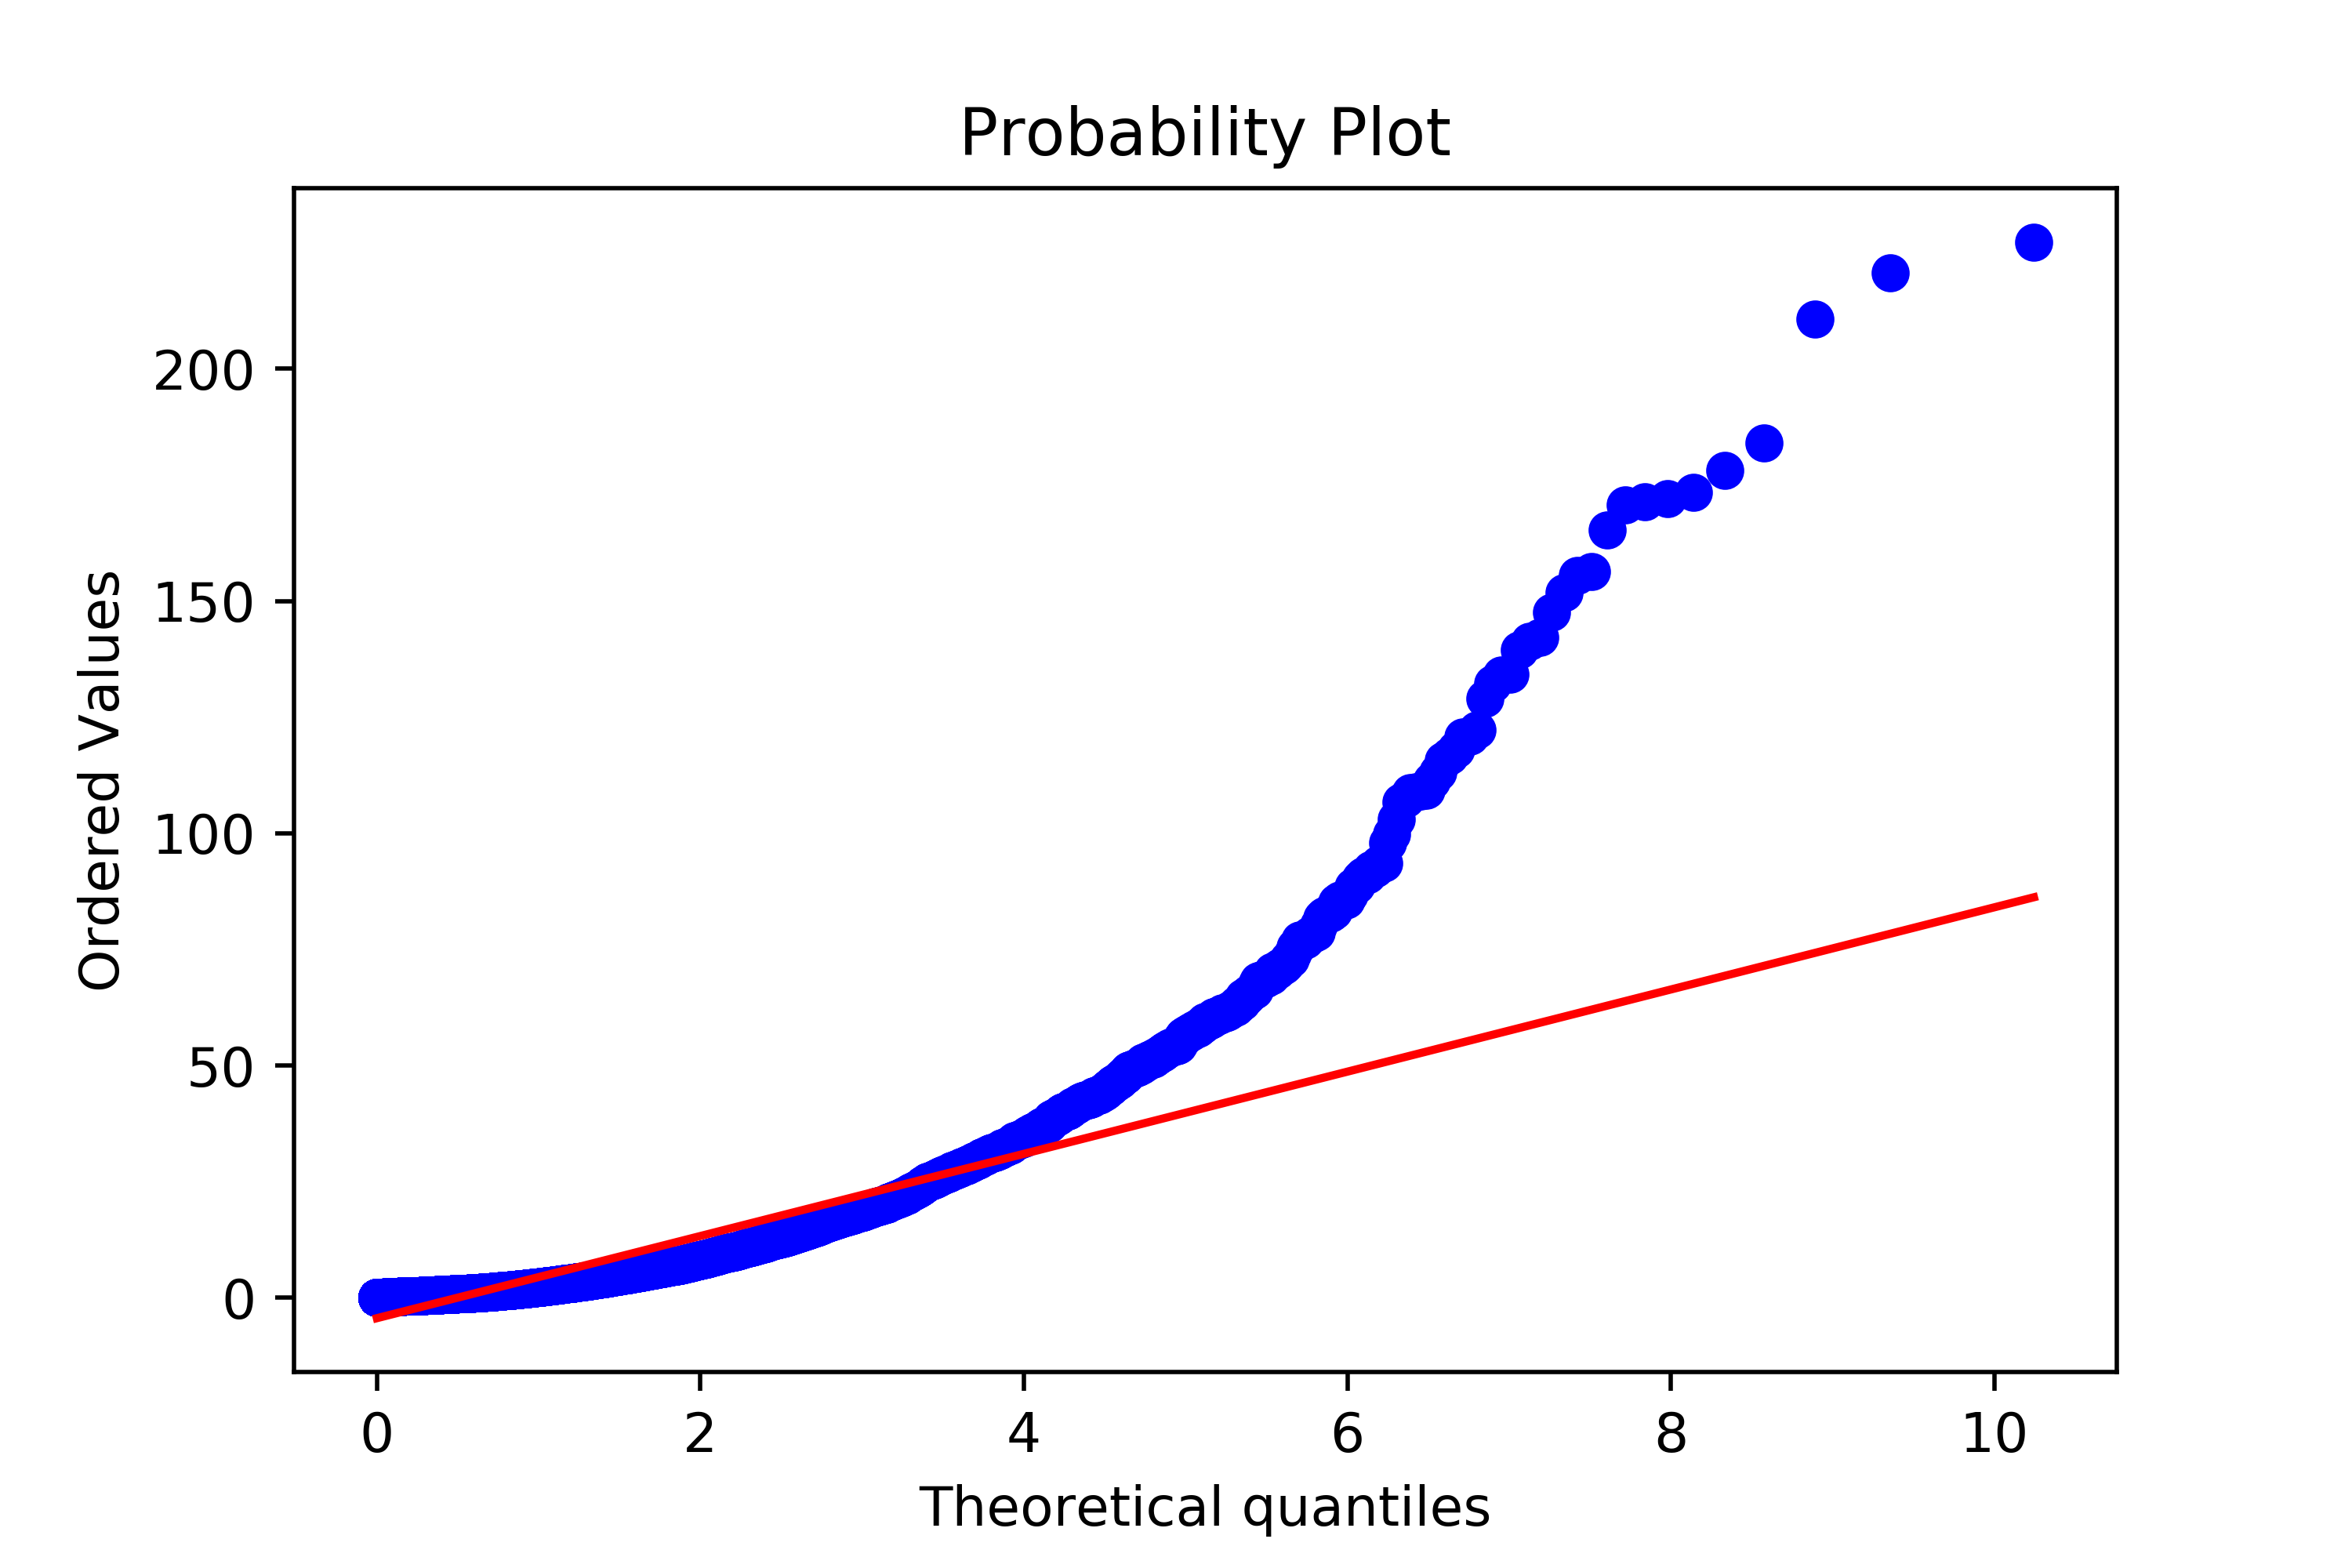
\includegraphics[width=60mm]{Figures/QQ_pos_k-2.png}}
{}
&
\subf{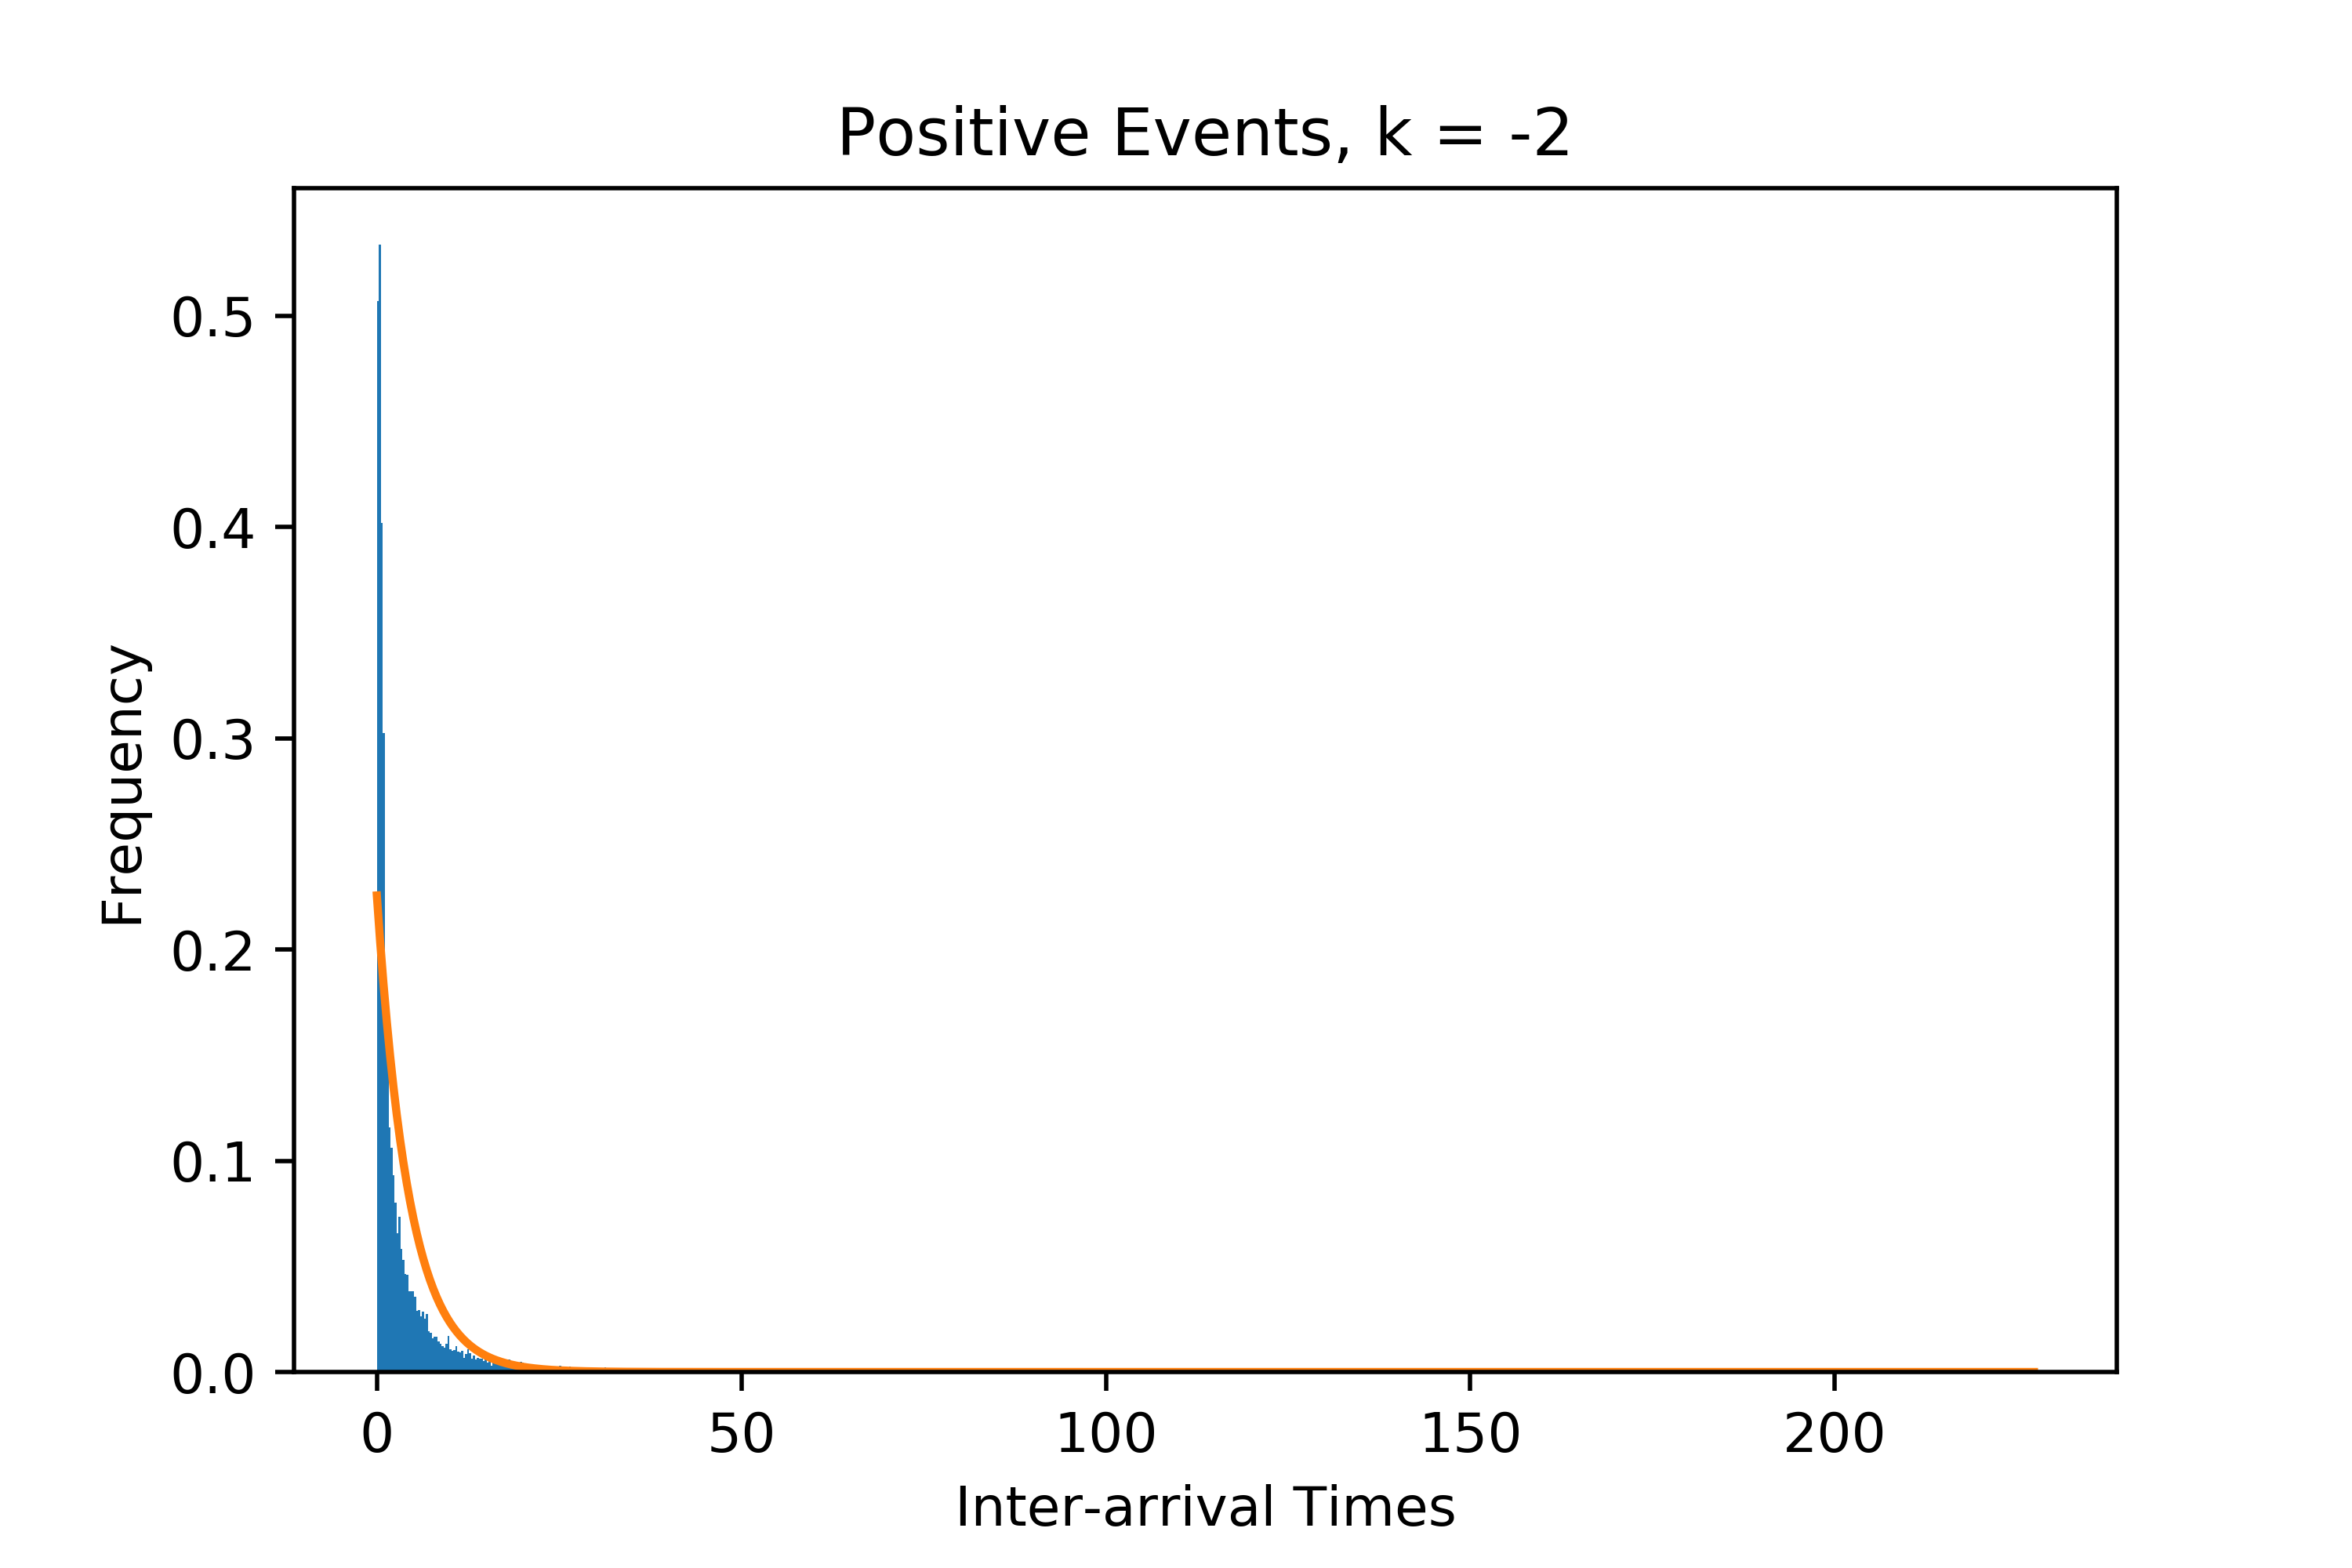
\includegraphics[width=60mm]{Figures/hist_pos_k-2.png}}
{}
\\
\subf{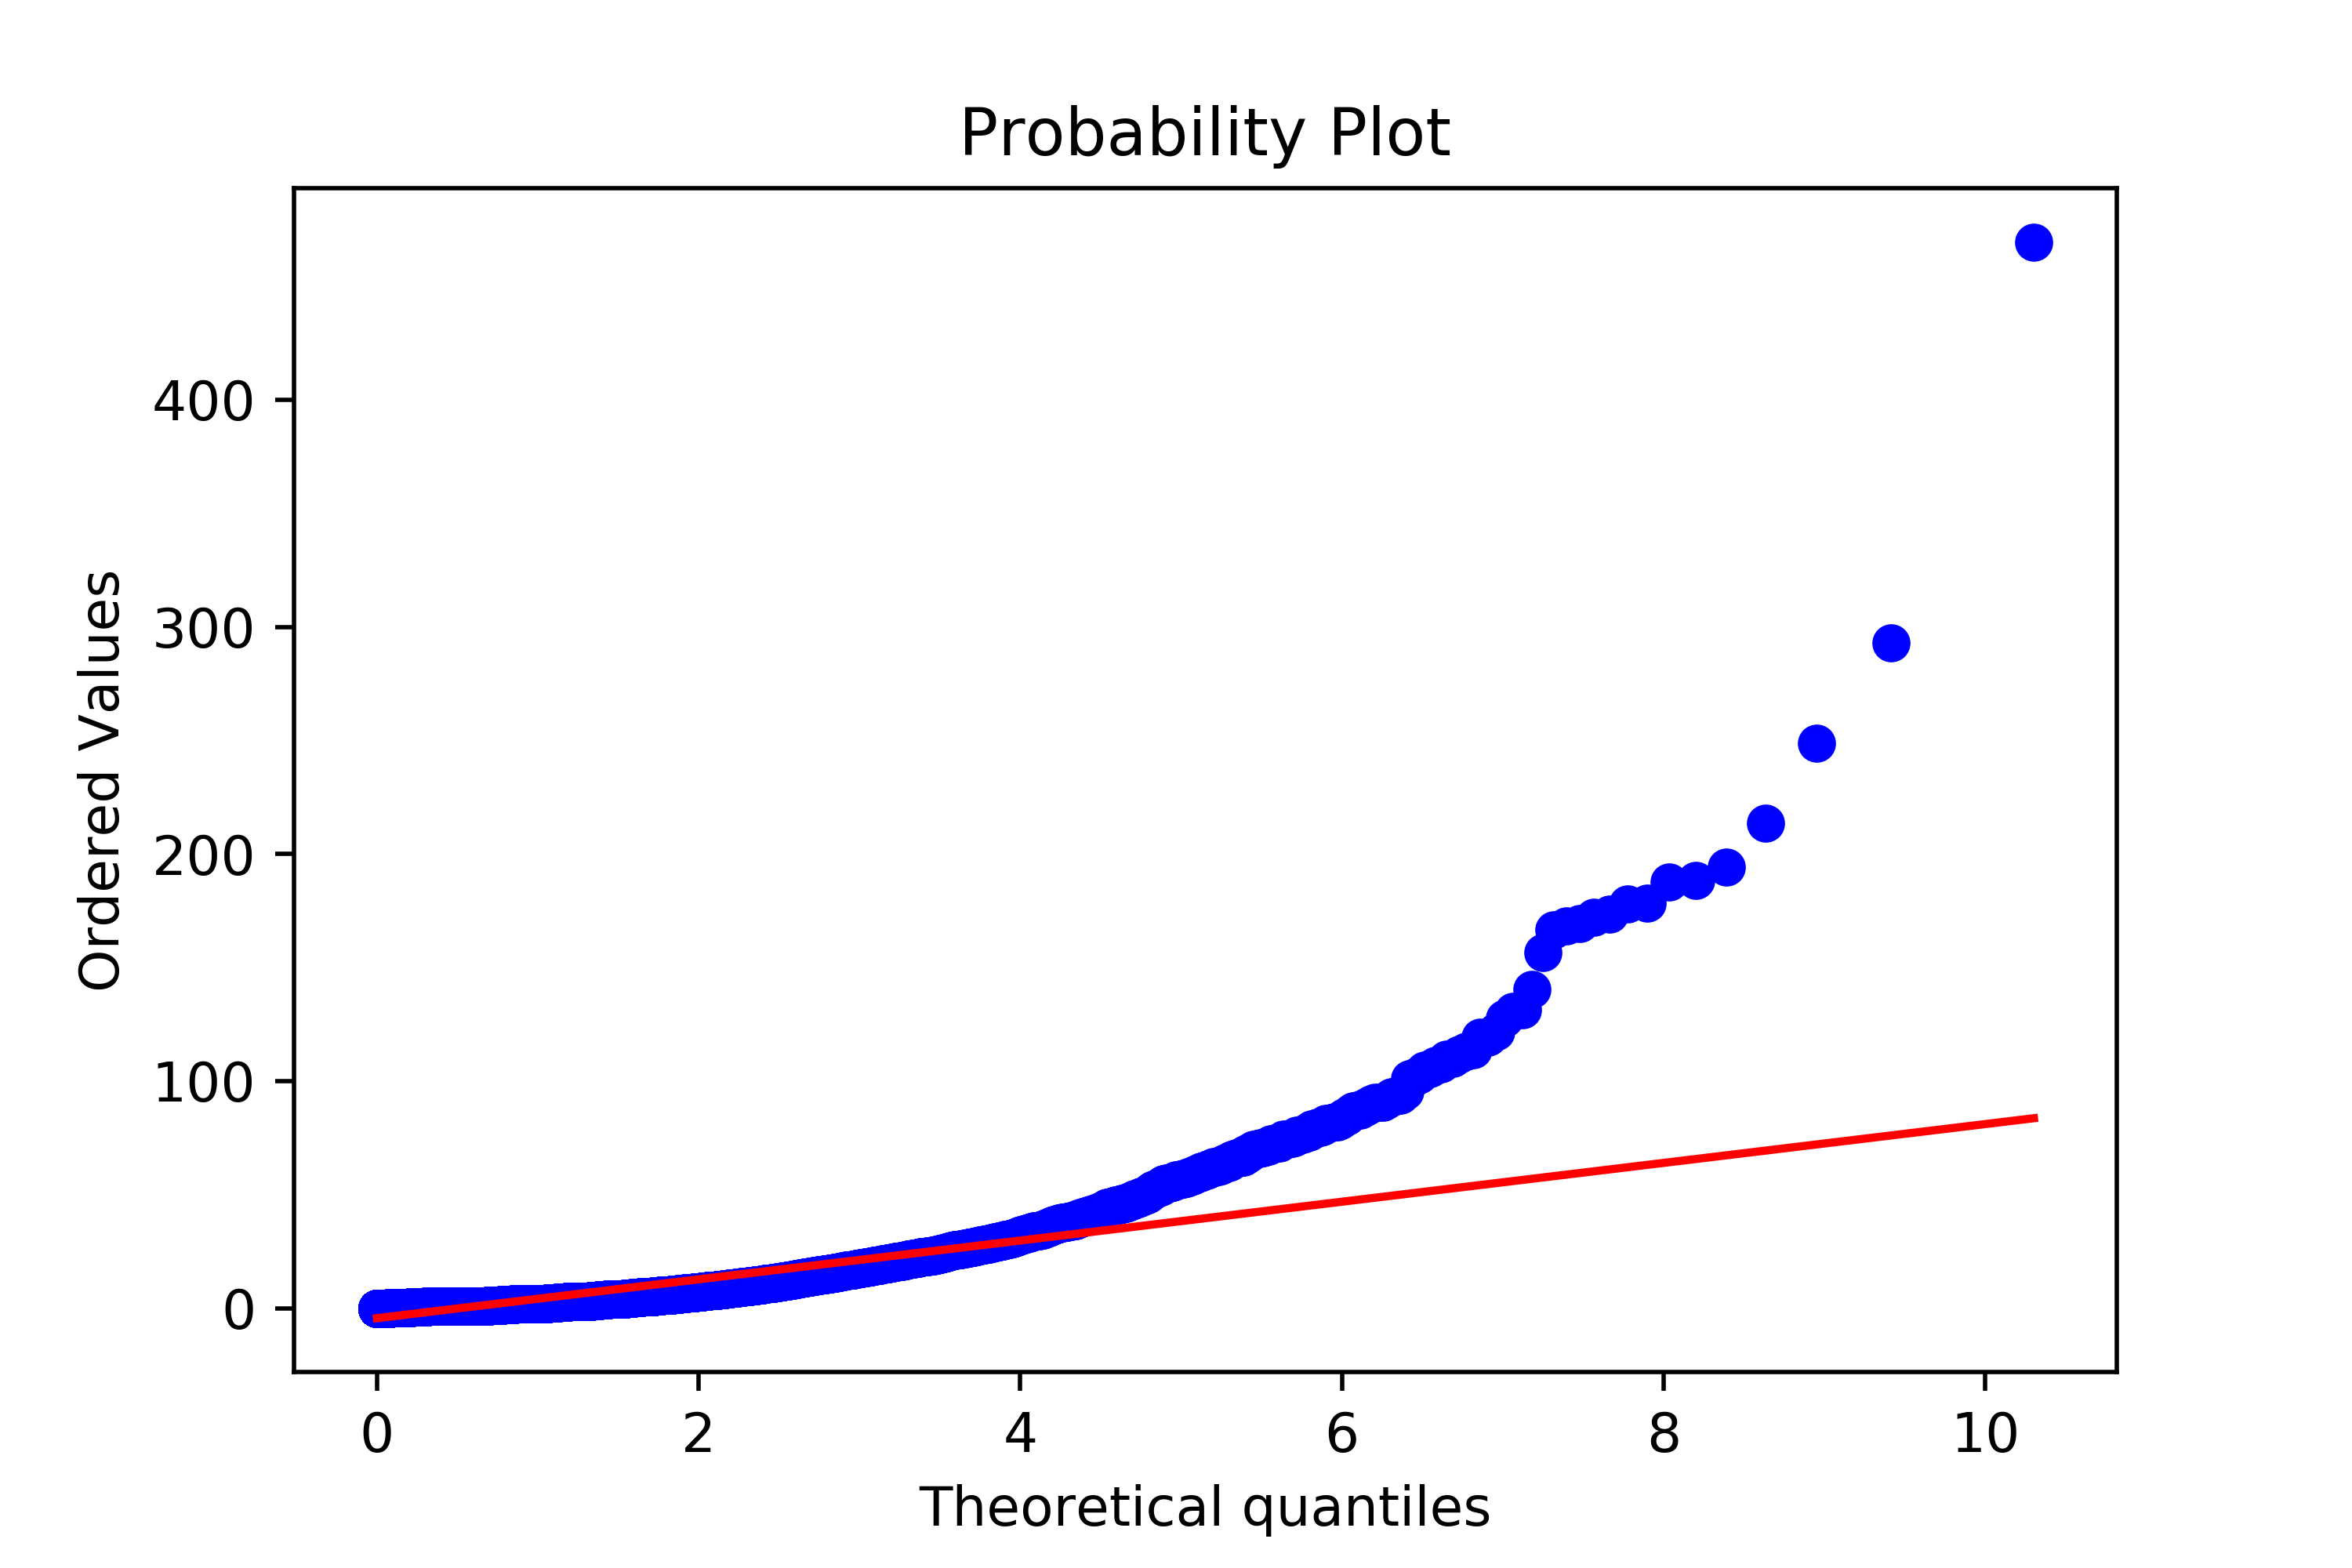
\includegraphics[width=60mm]{Figures/QQ_pos_k-1.png}}
{}
&
\subf{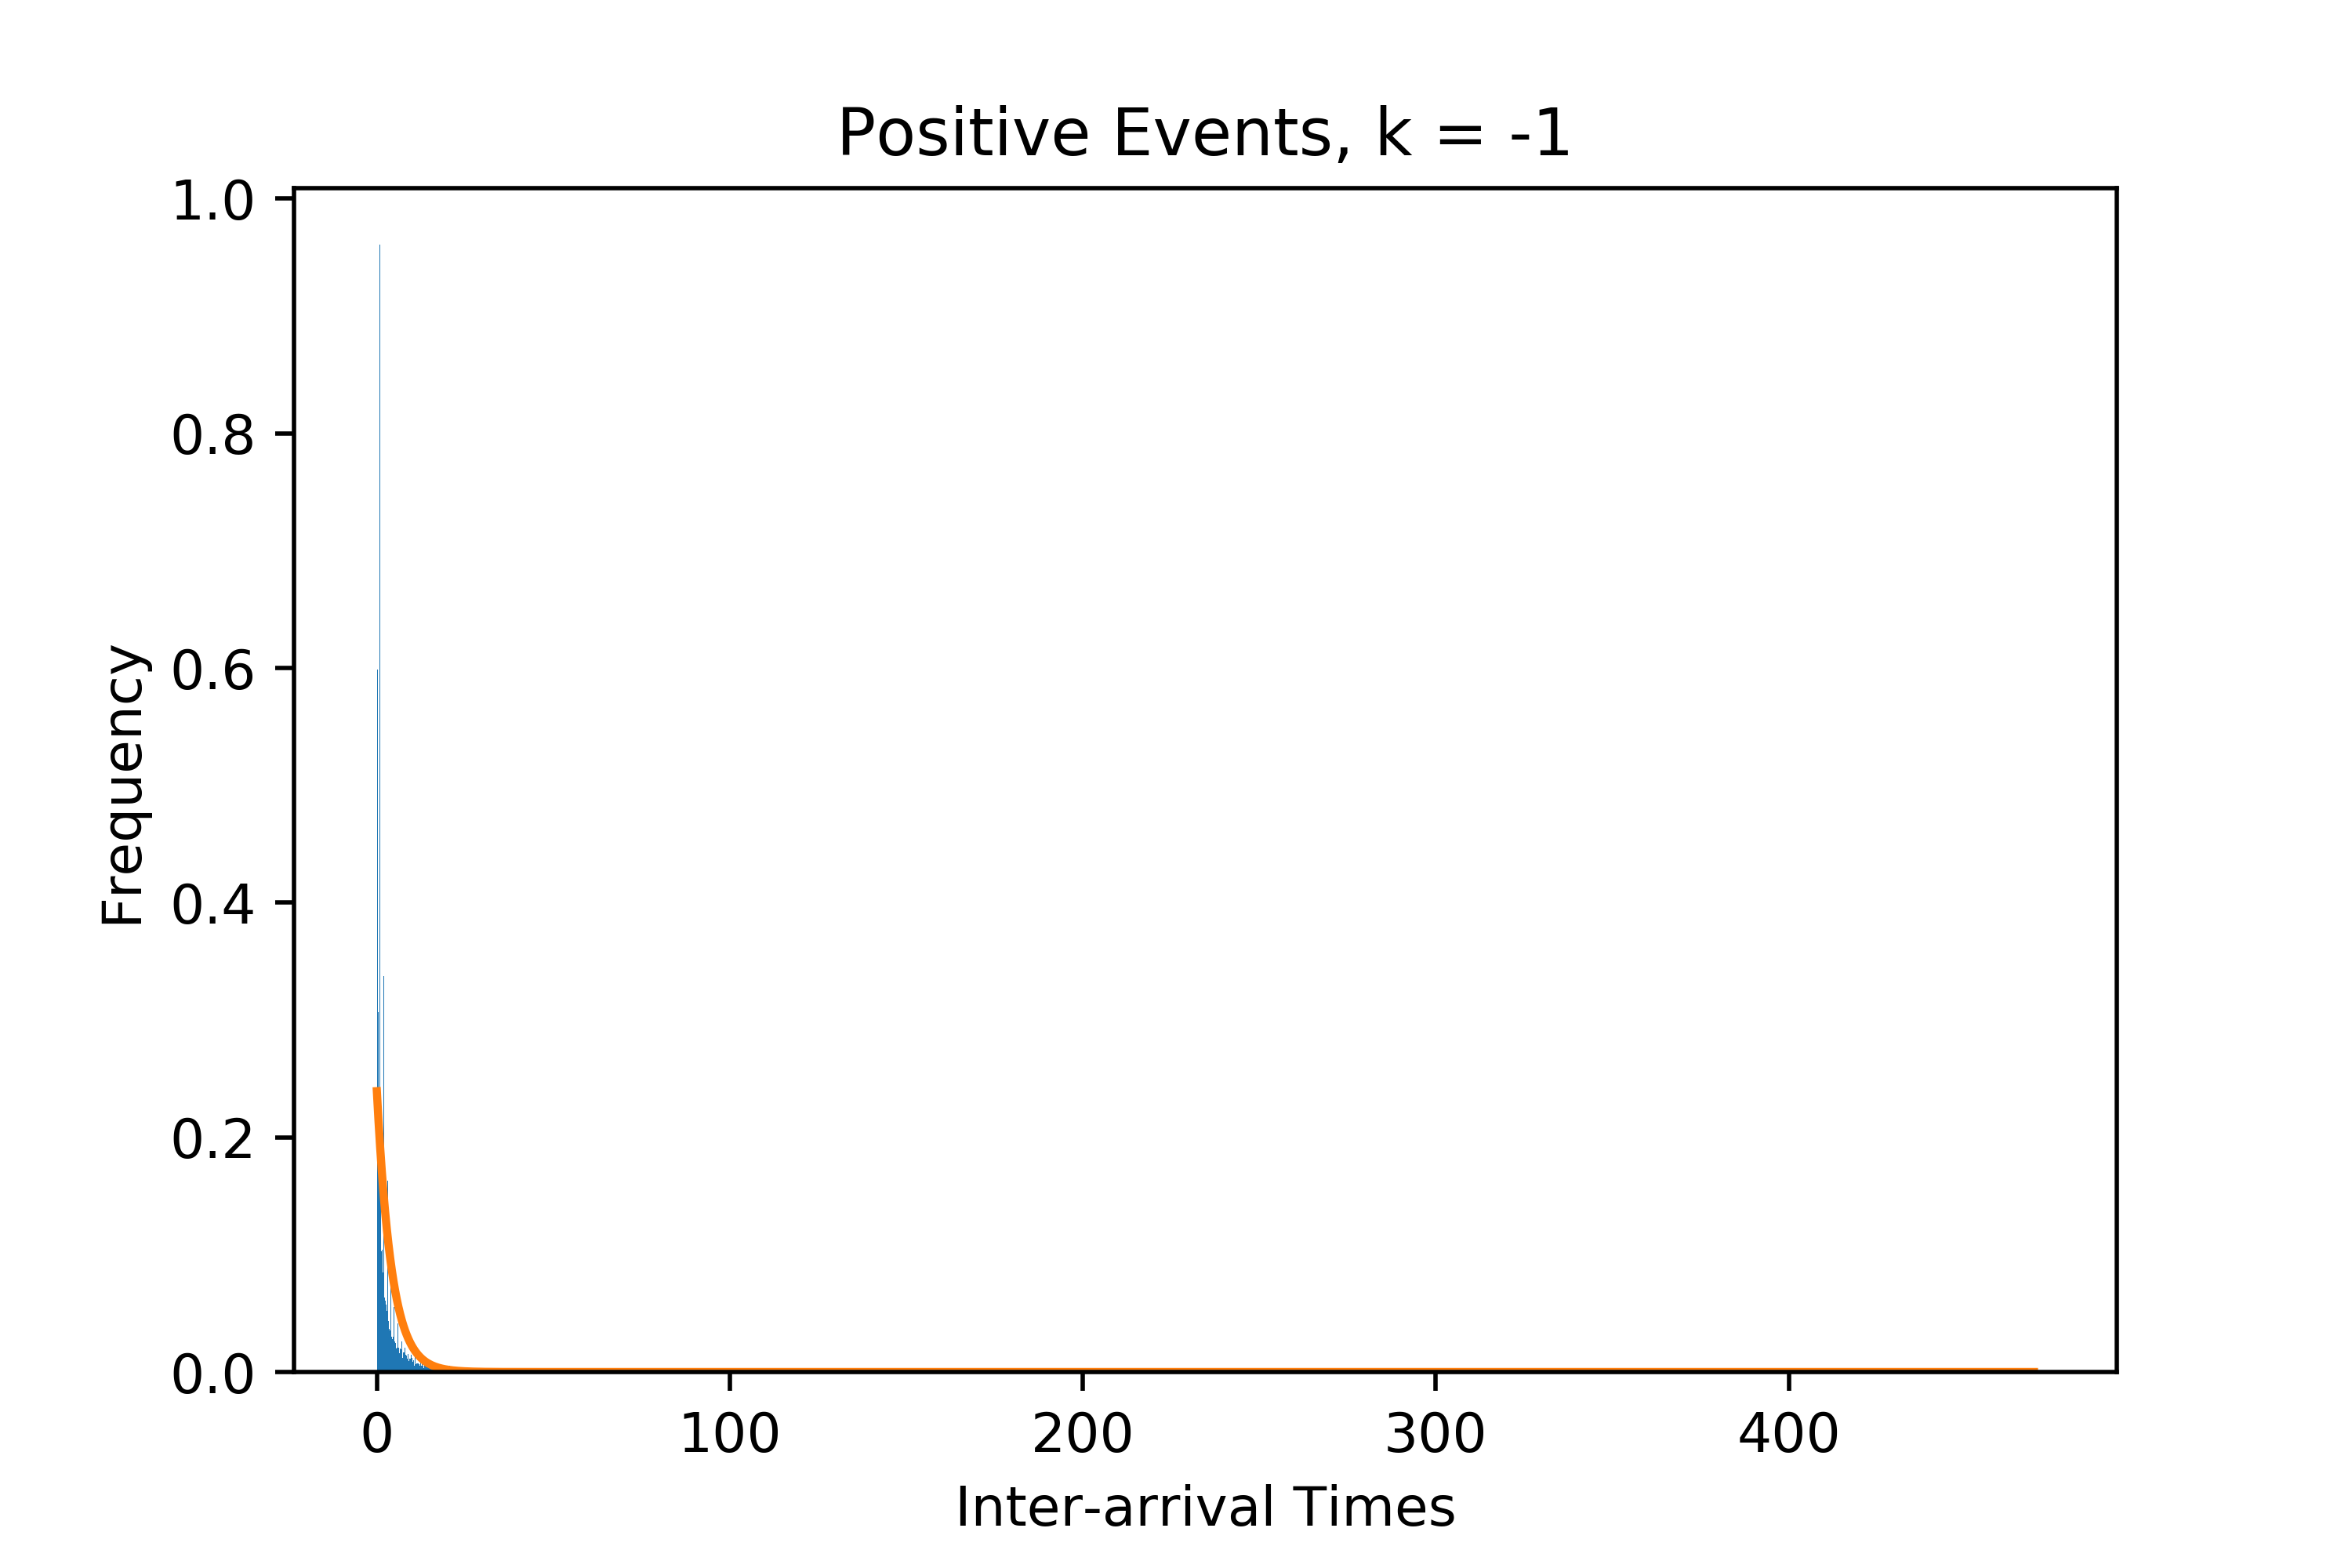
\includegraphics[width=60mm]{Figures/hist_pos_k-1.png}}
{}
\\
\subf{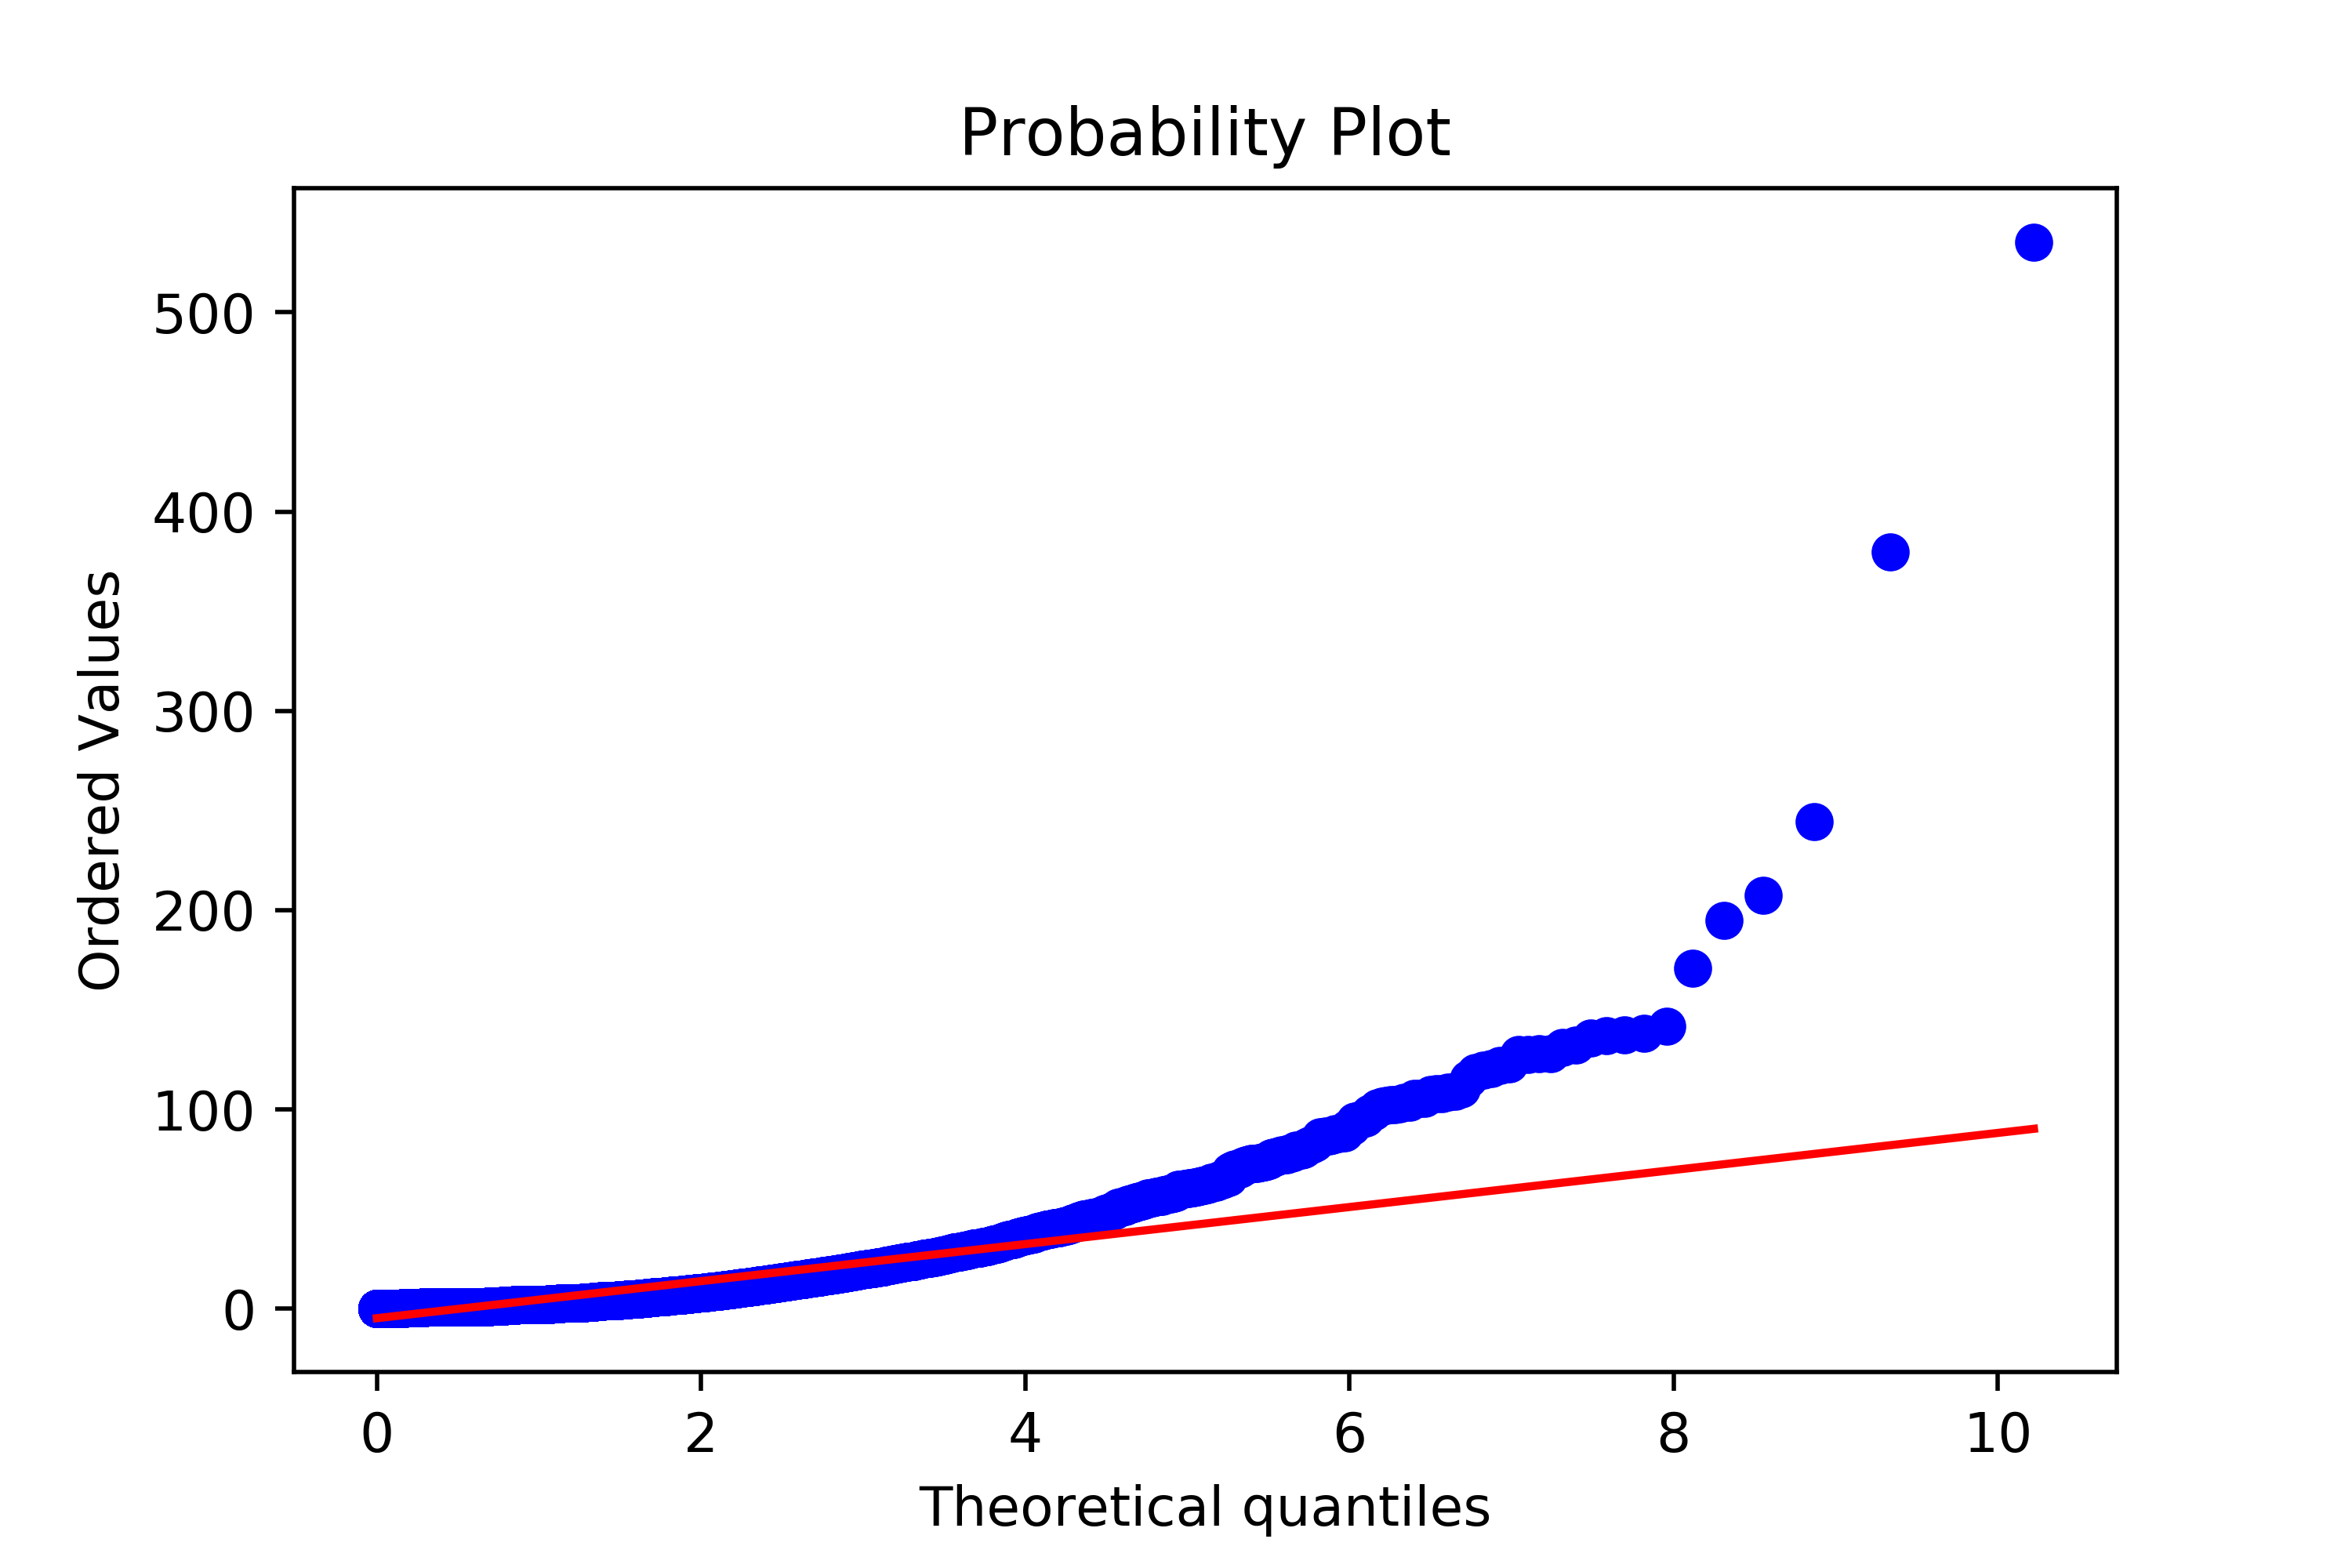
\includegraphics[width=60mm]{Figures/QQ_pos_k1.png}}
{}
&
\subf{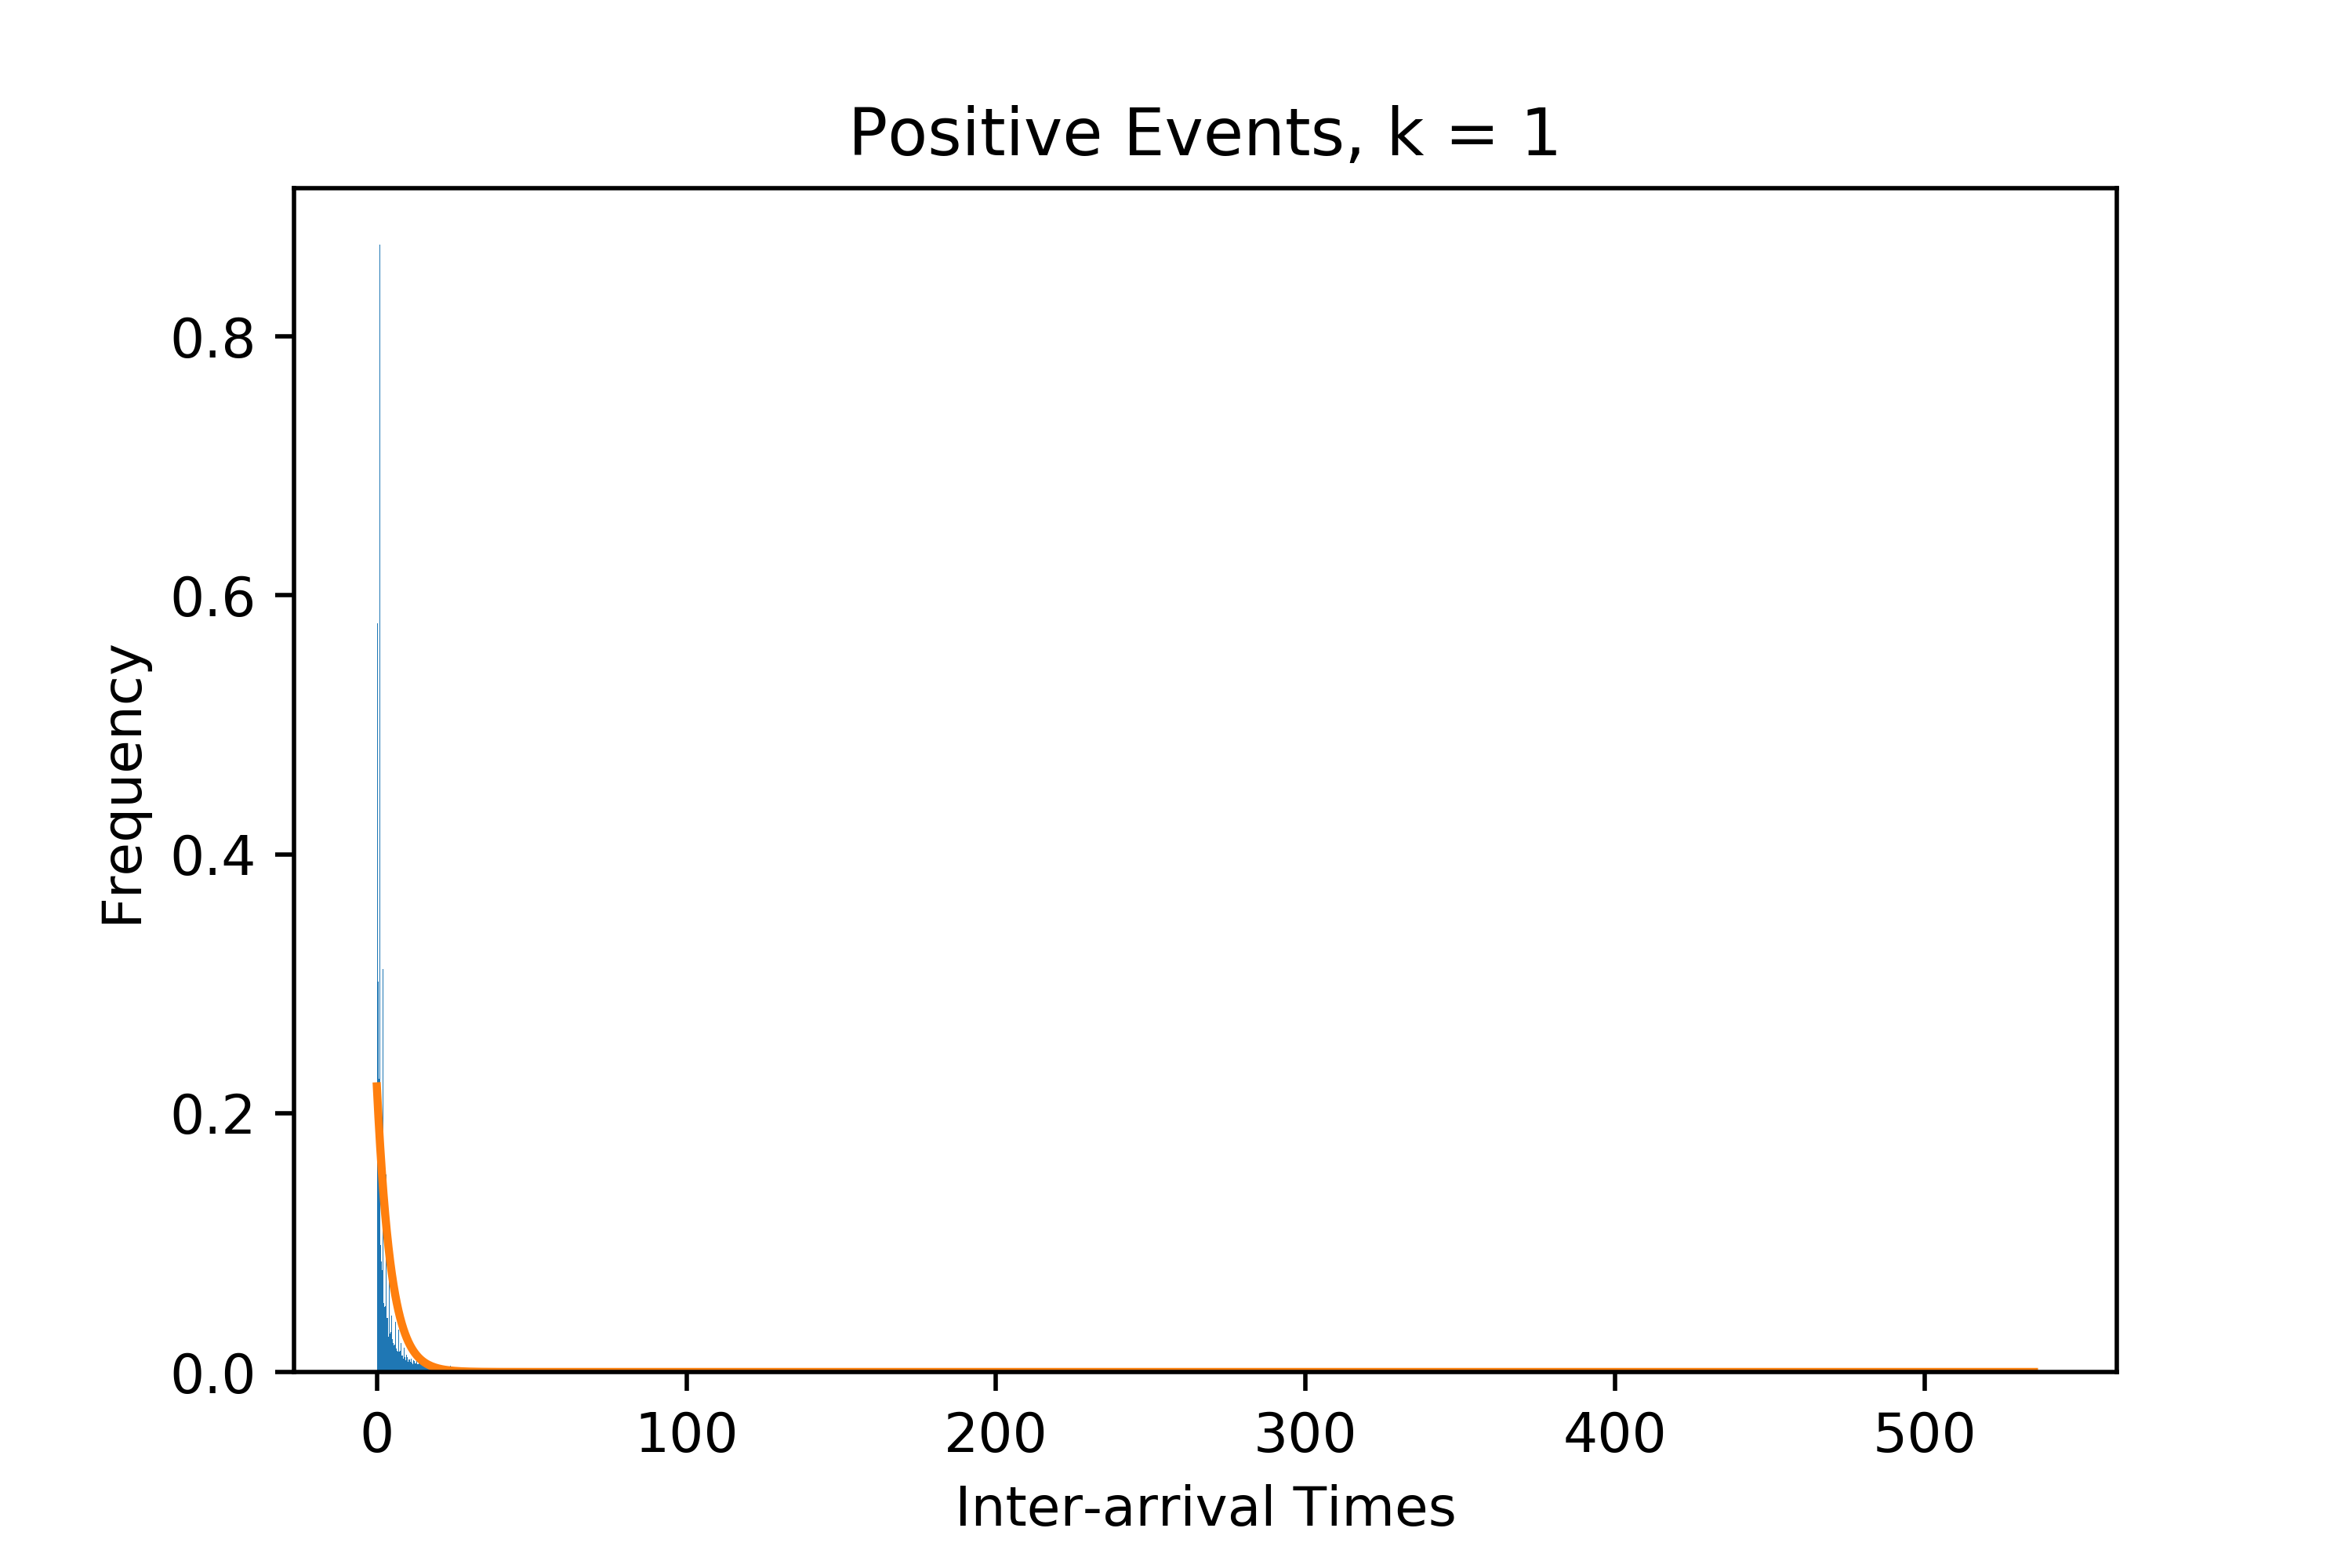
\includegraphics[width=60mm]{Figures/hist_pos_k1.png}}
{}
\\
\subf{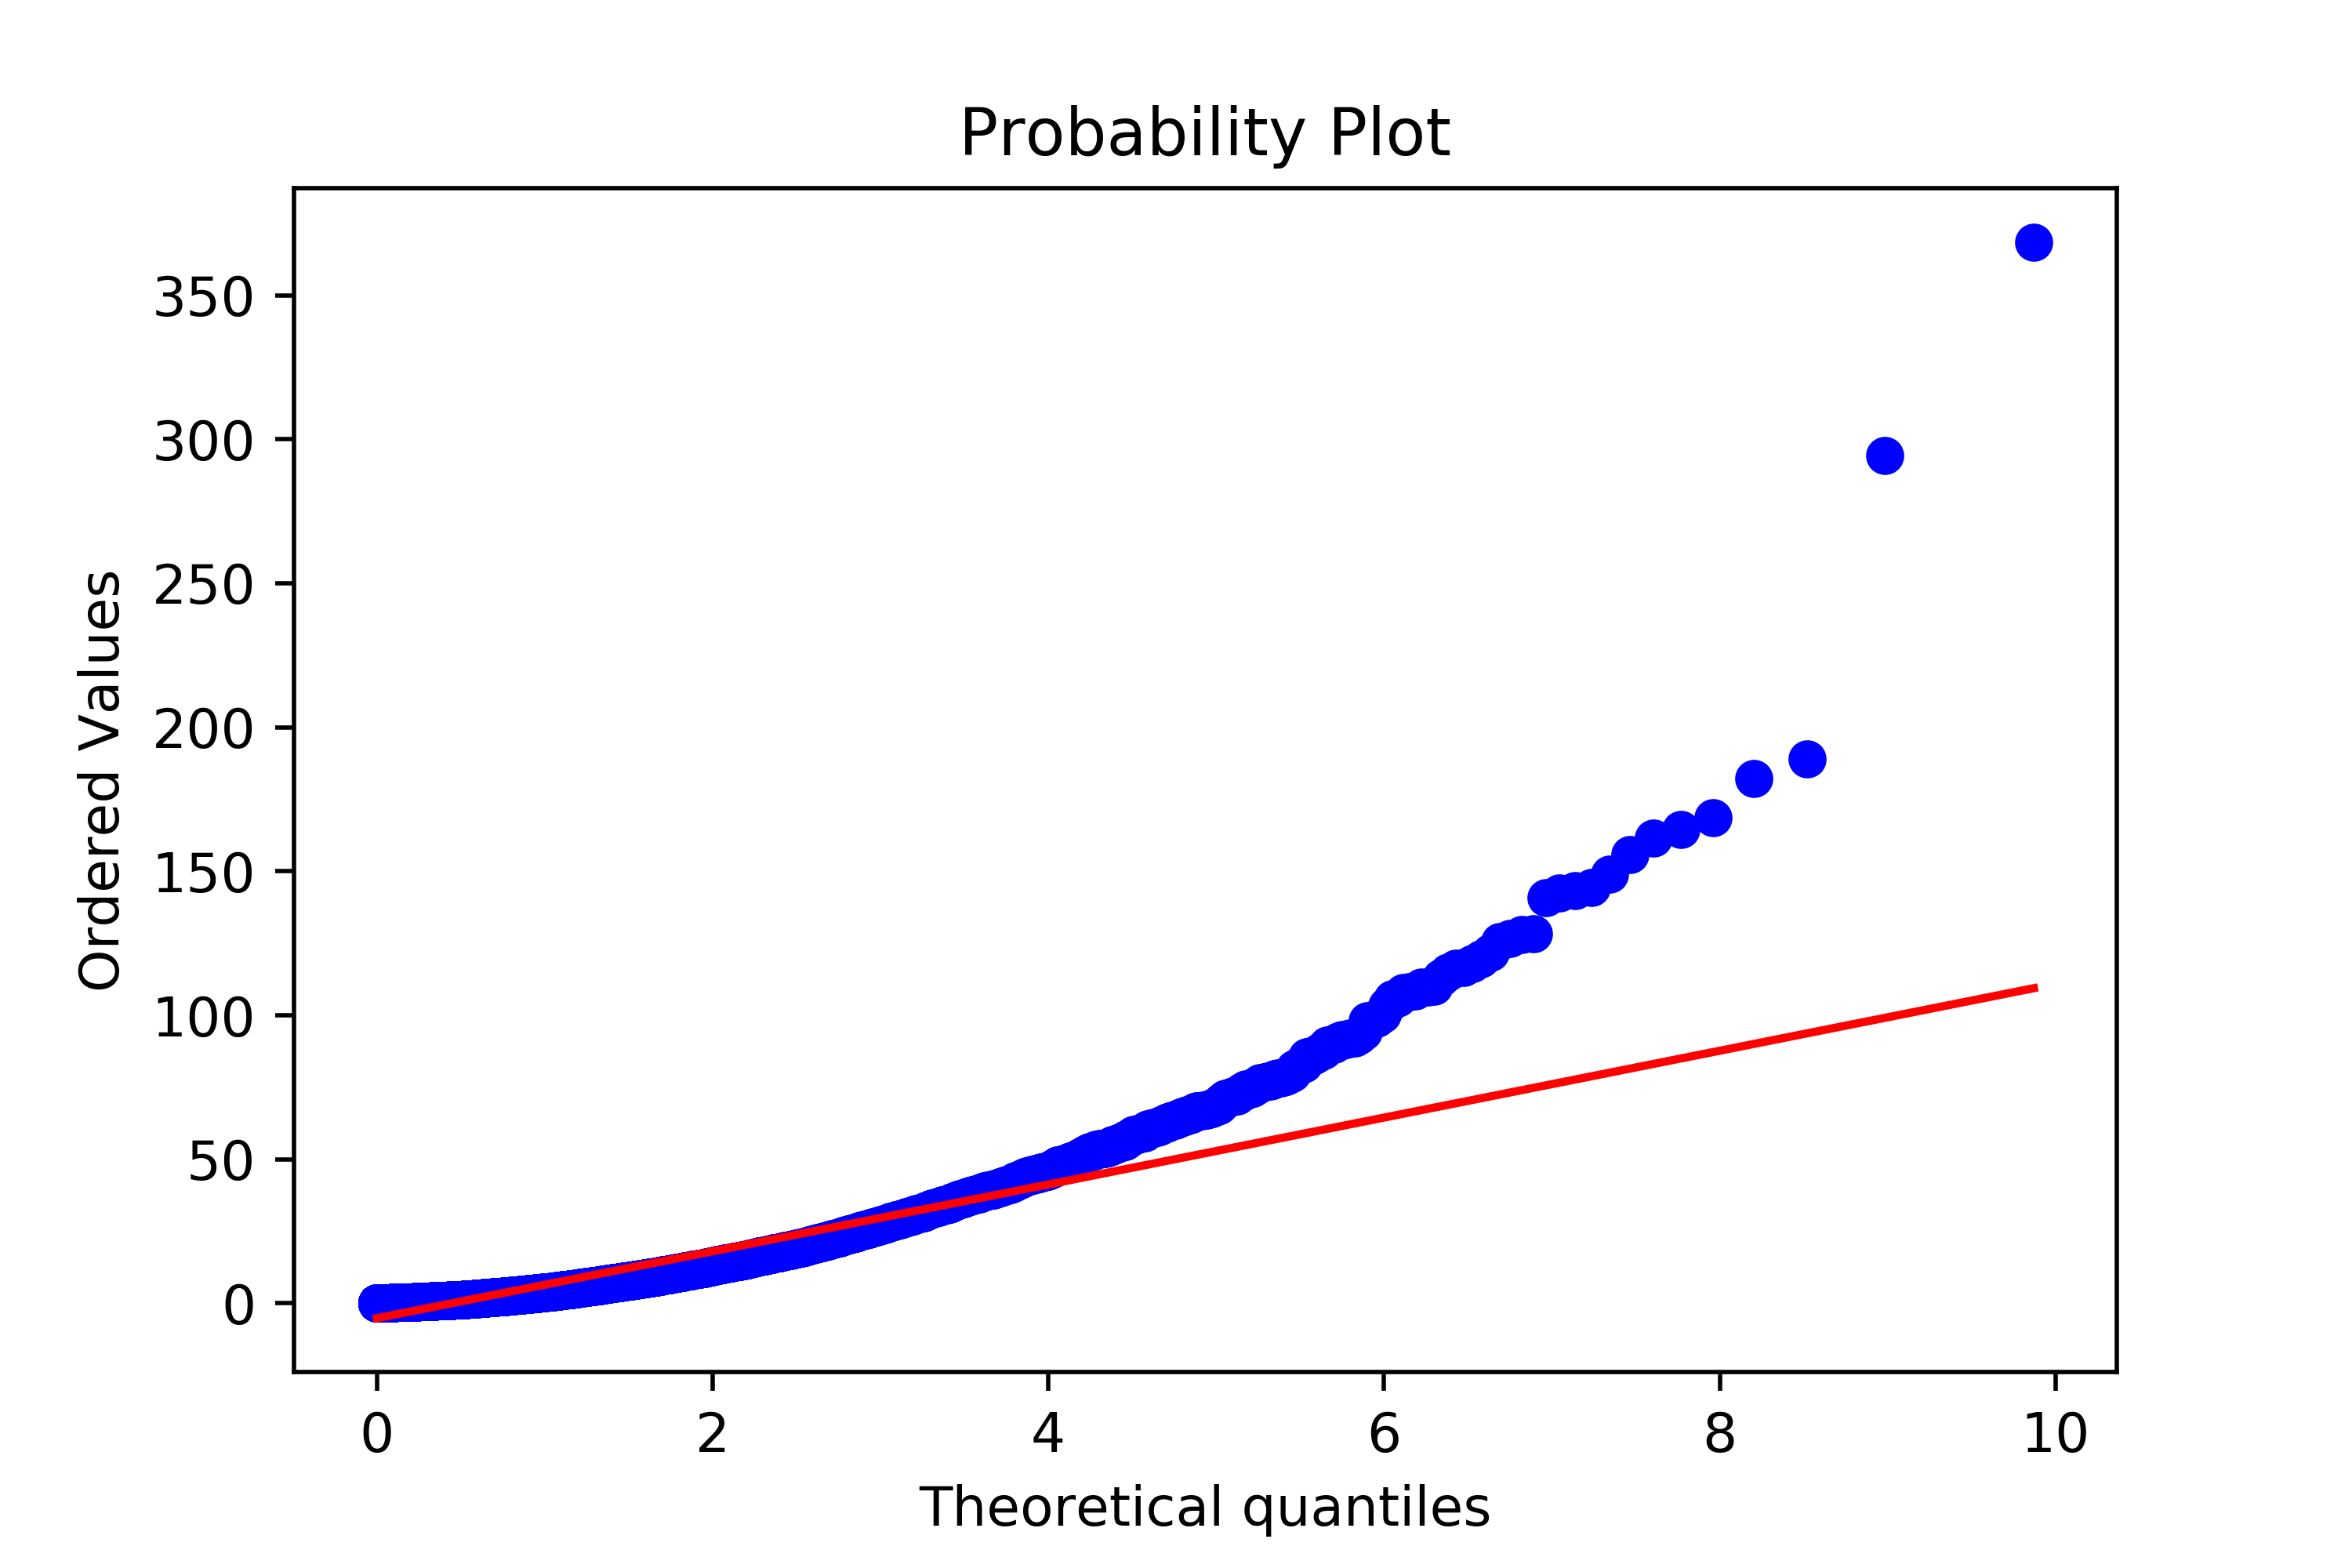
\includegraphics[width=60mm]{Figures/QQ_pos_k2.png}}
{}
&
\subf{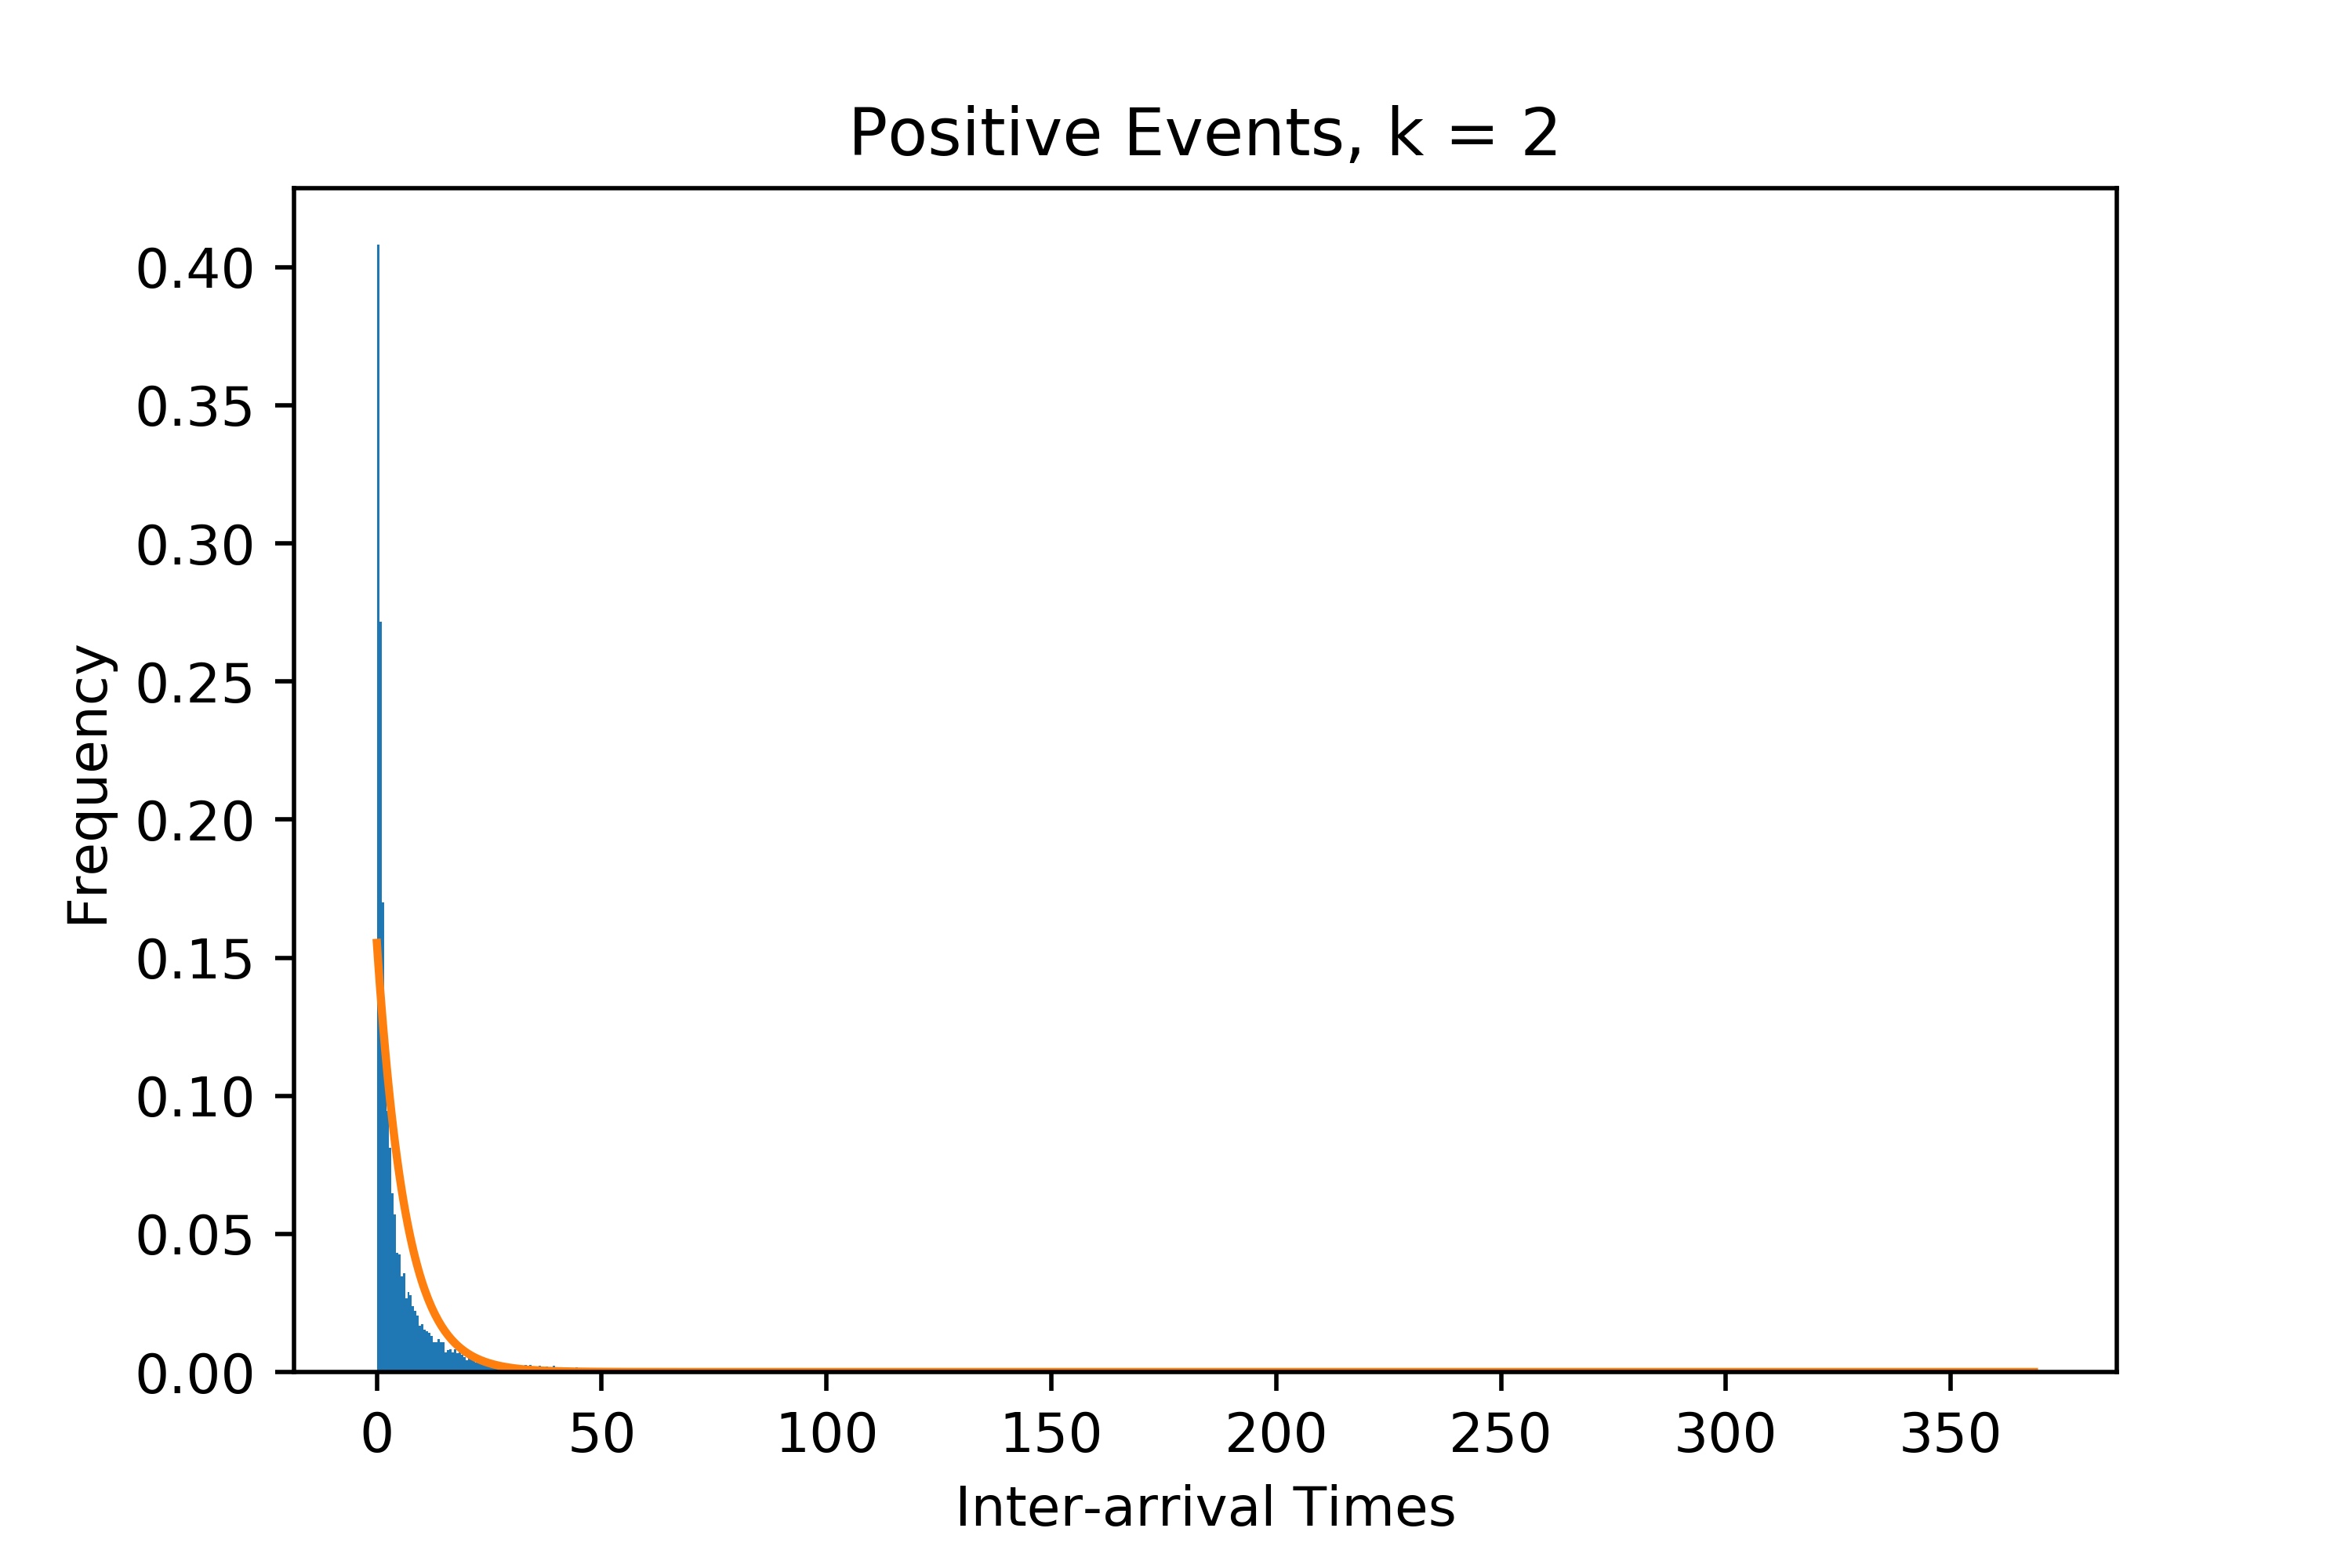
\includegraphics[width=60mm]{Figures/hist_pos_k2.png}}
{}
\\
\hline
\end{tabular}
\label{fig:interarrivals_pos}
\end{figure}

\begin{figure}
\centering
\caption{Inter-Arrival Times for Negative Events Compared to Exponential Distribution (4 Positions Closest to $p_0$)}
\begin{tabular}{cc}
\hline
\subf{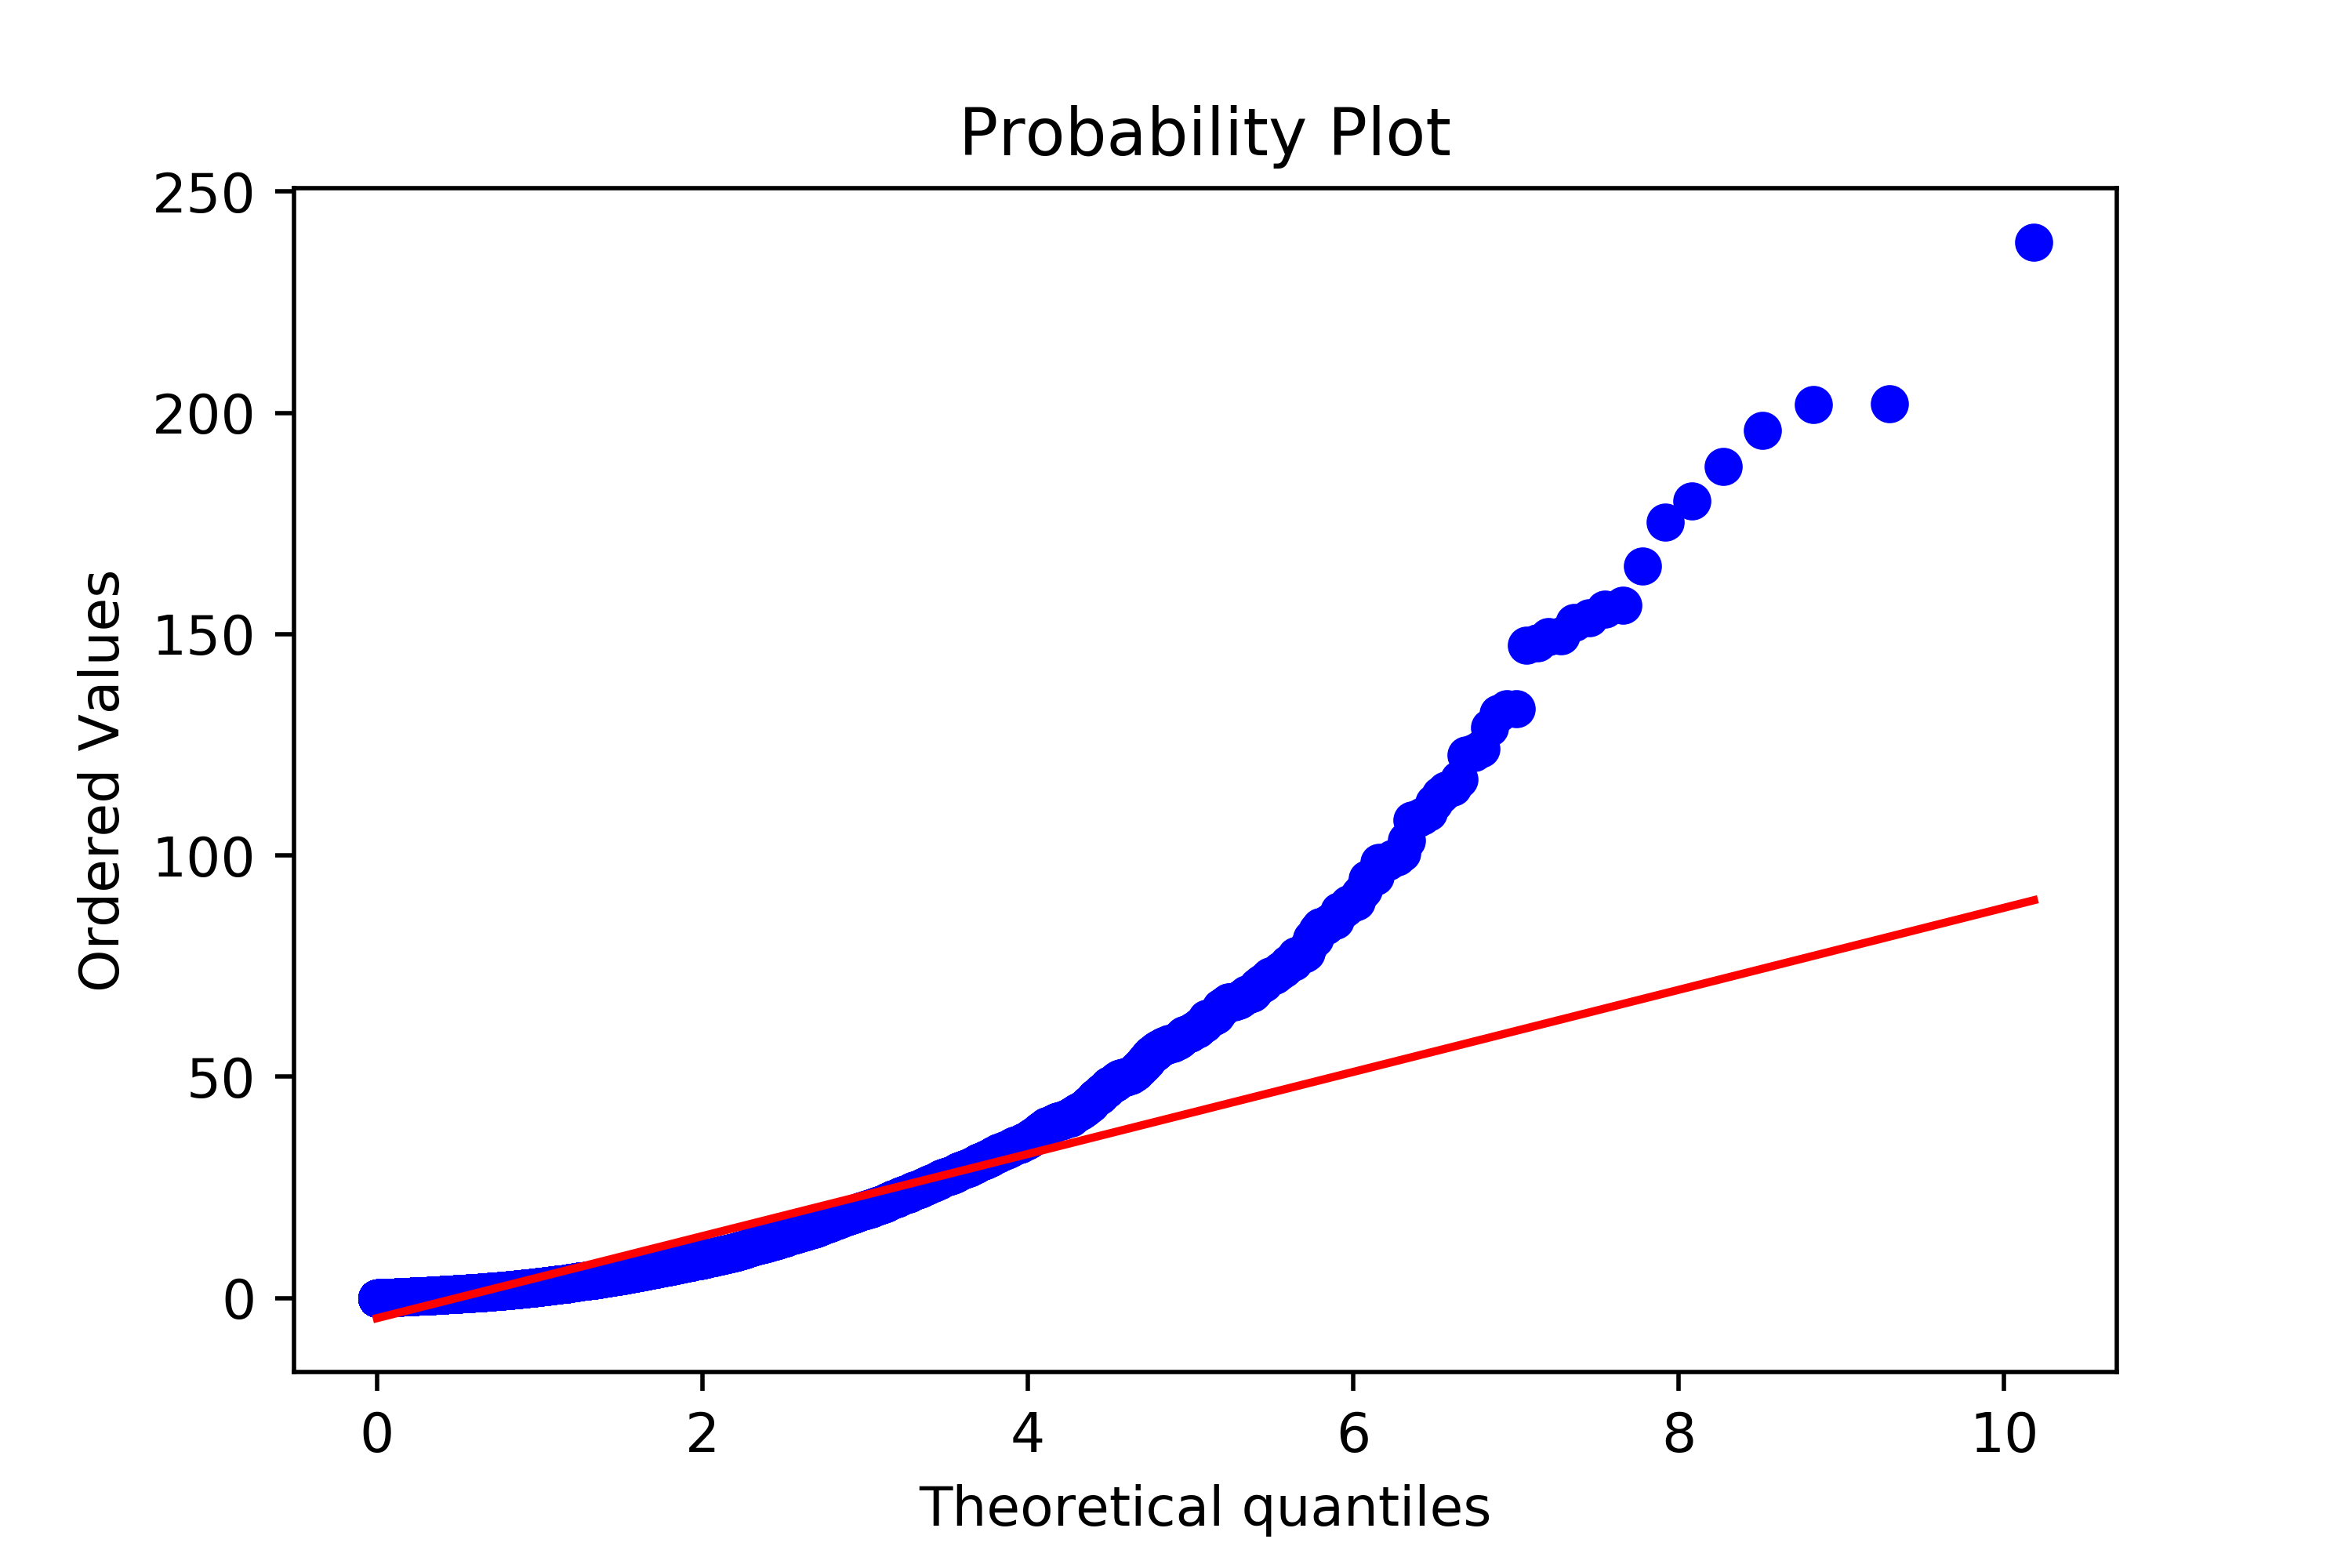
\includegraphics[width=60mm]{Figures/QQ_neg_k-2.png}}
{}
&
\subf{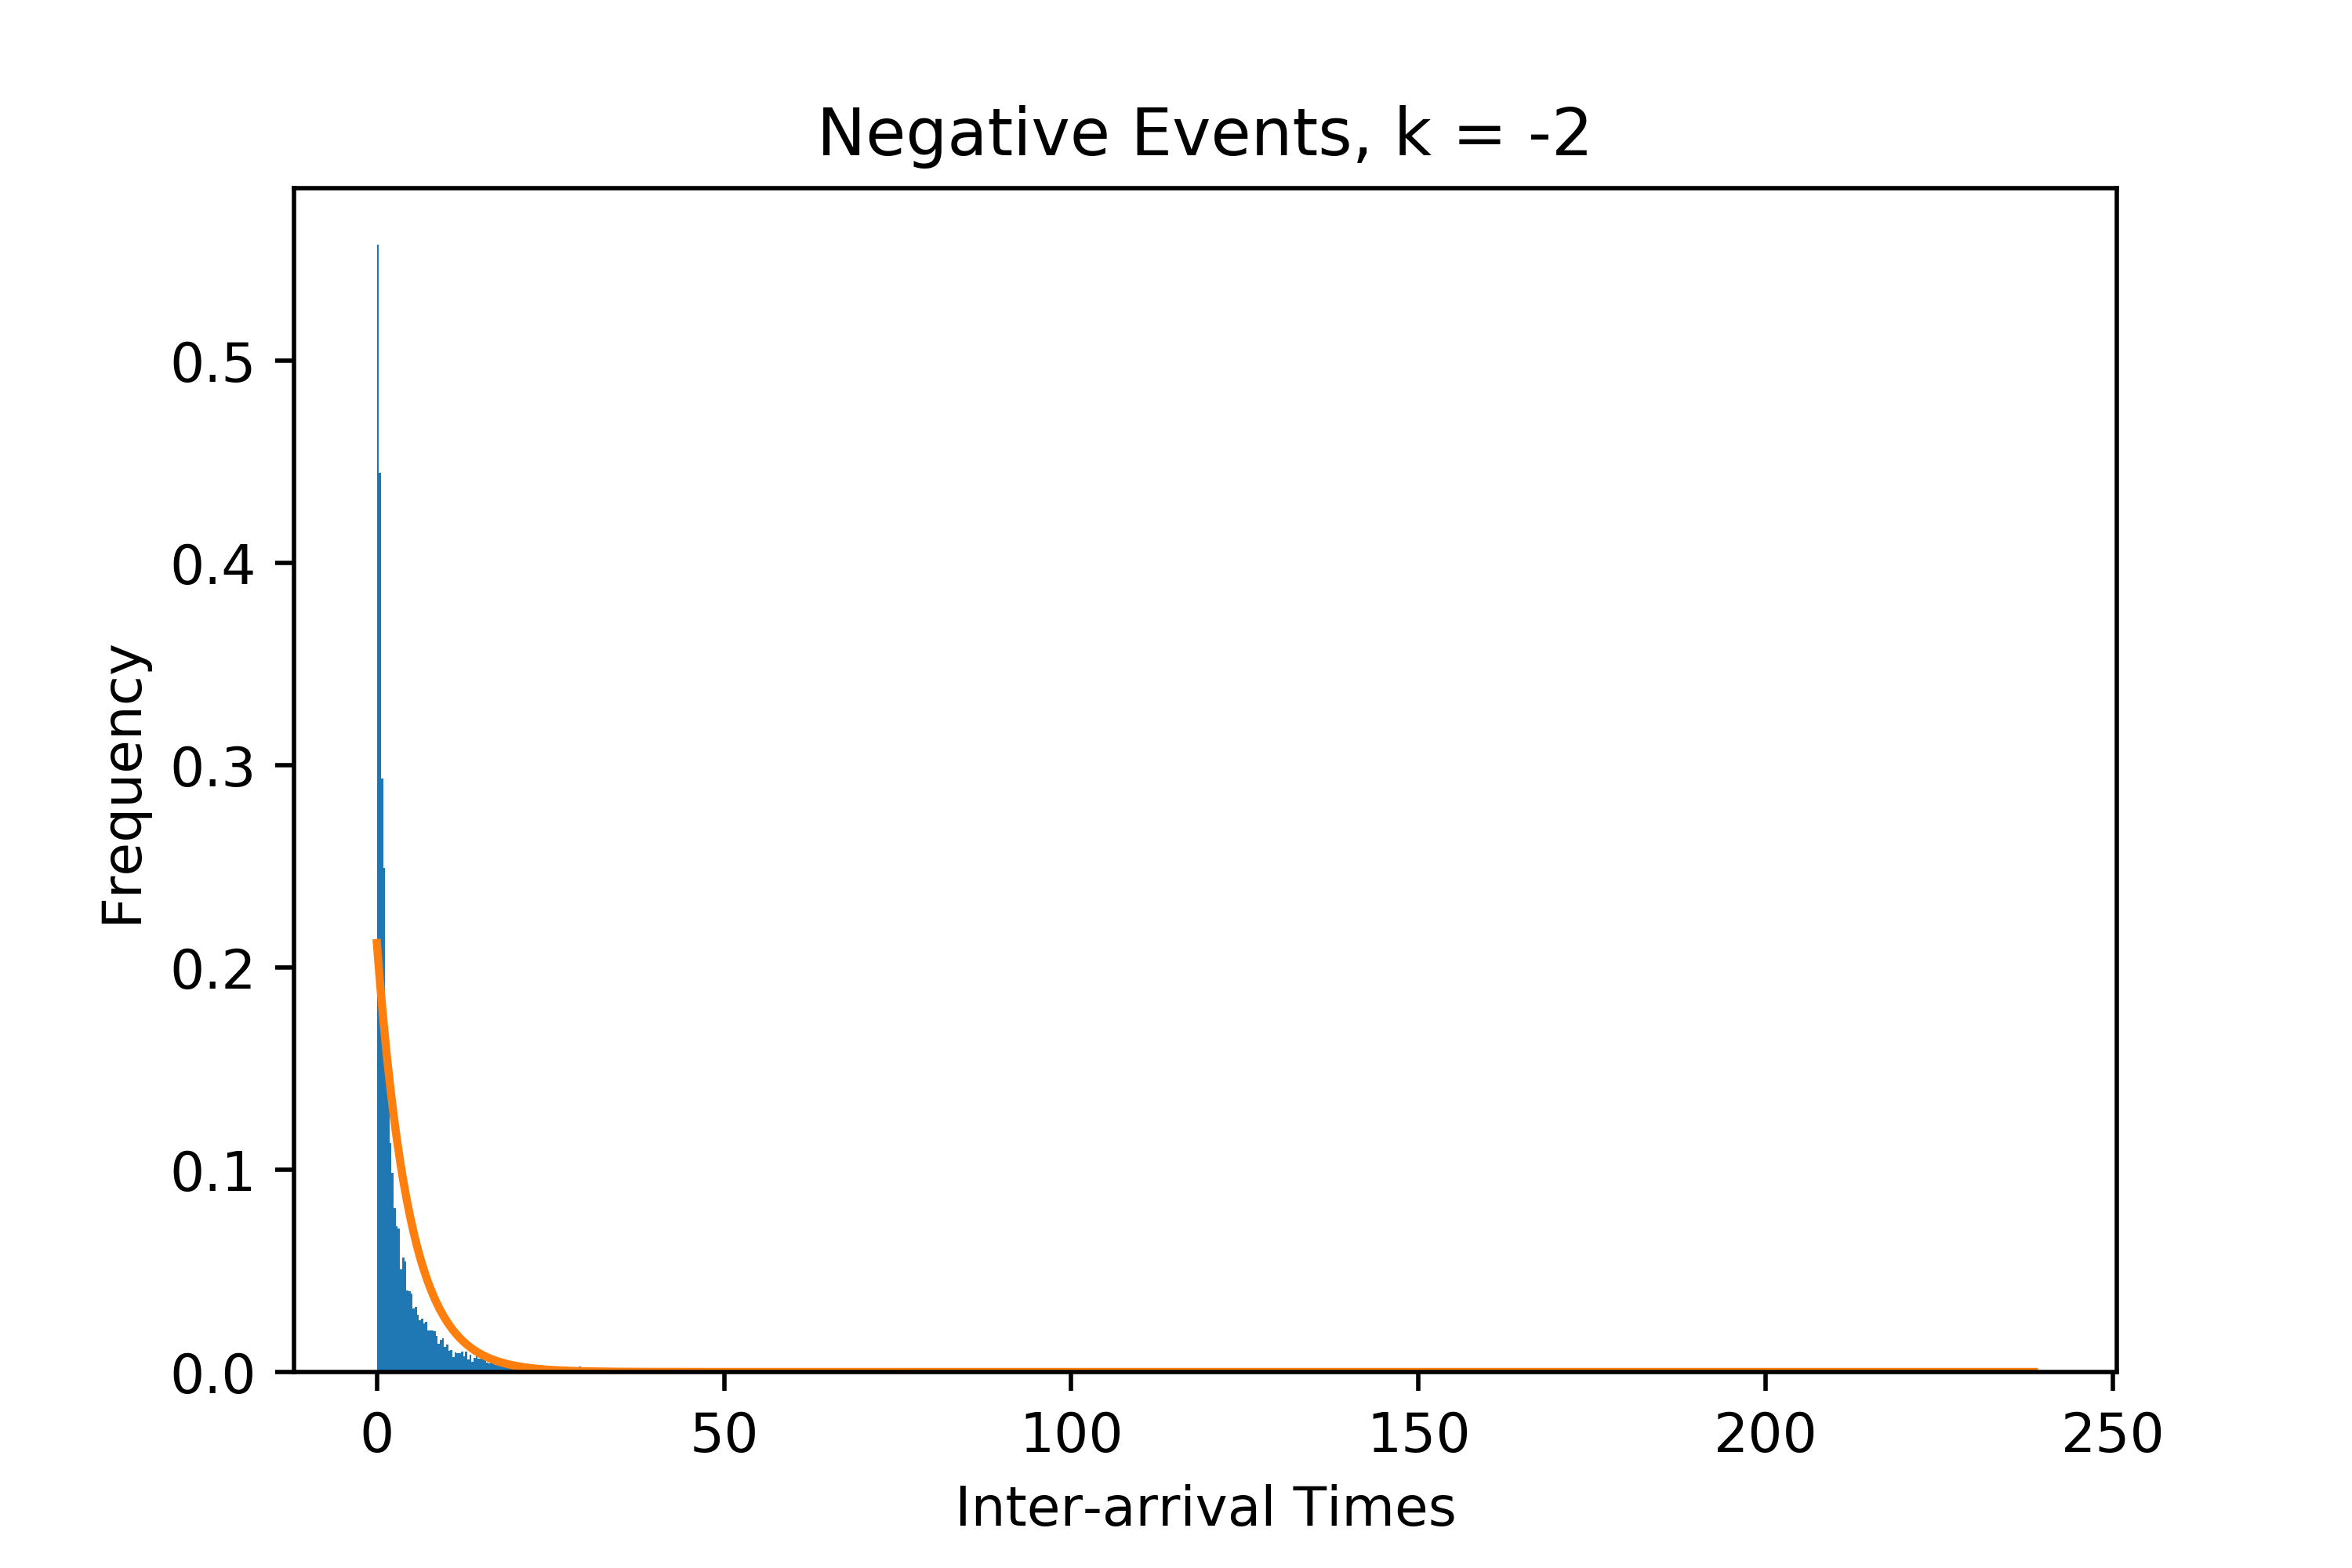
\includegraphics[width=60mm]{Figures/hist_neg_k-2.png}}
{}
\\
\subf{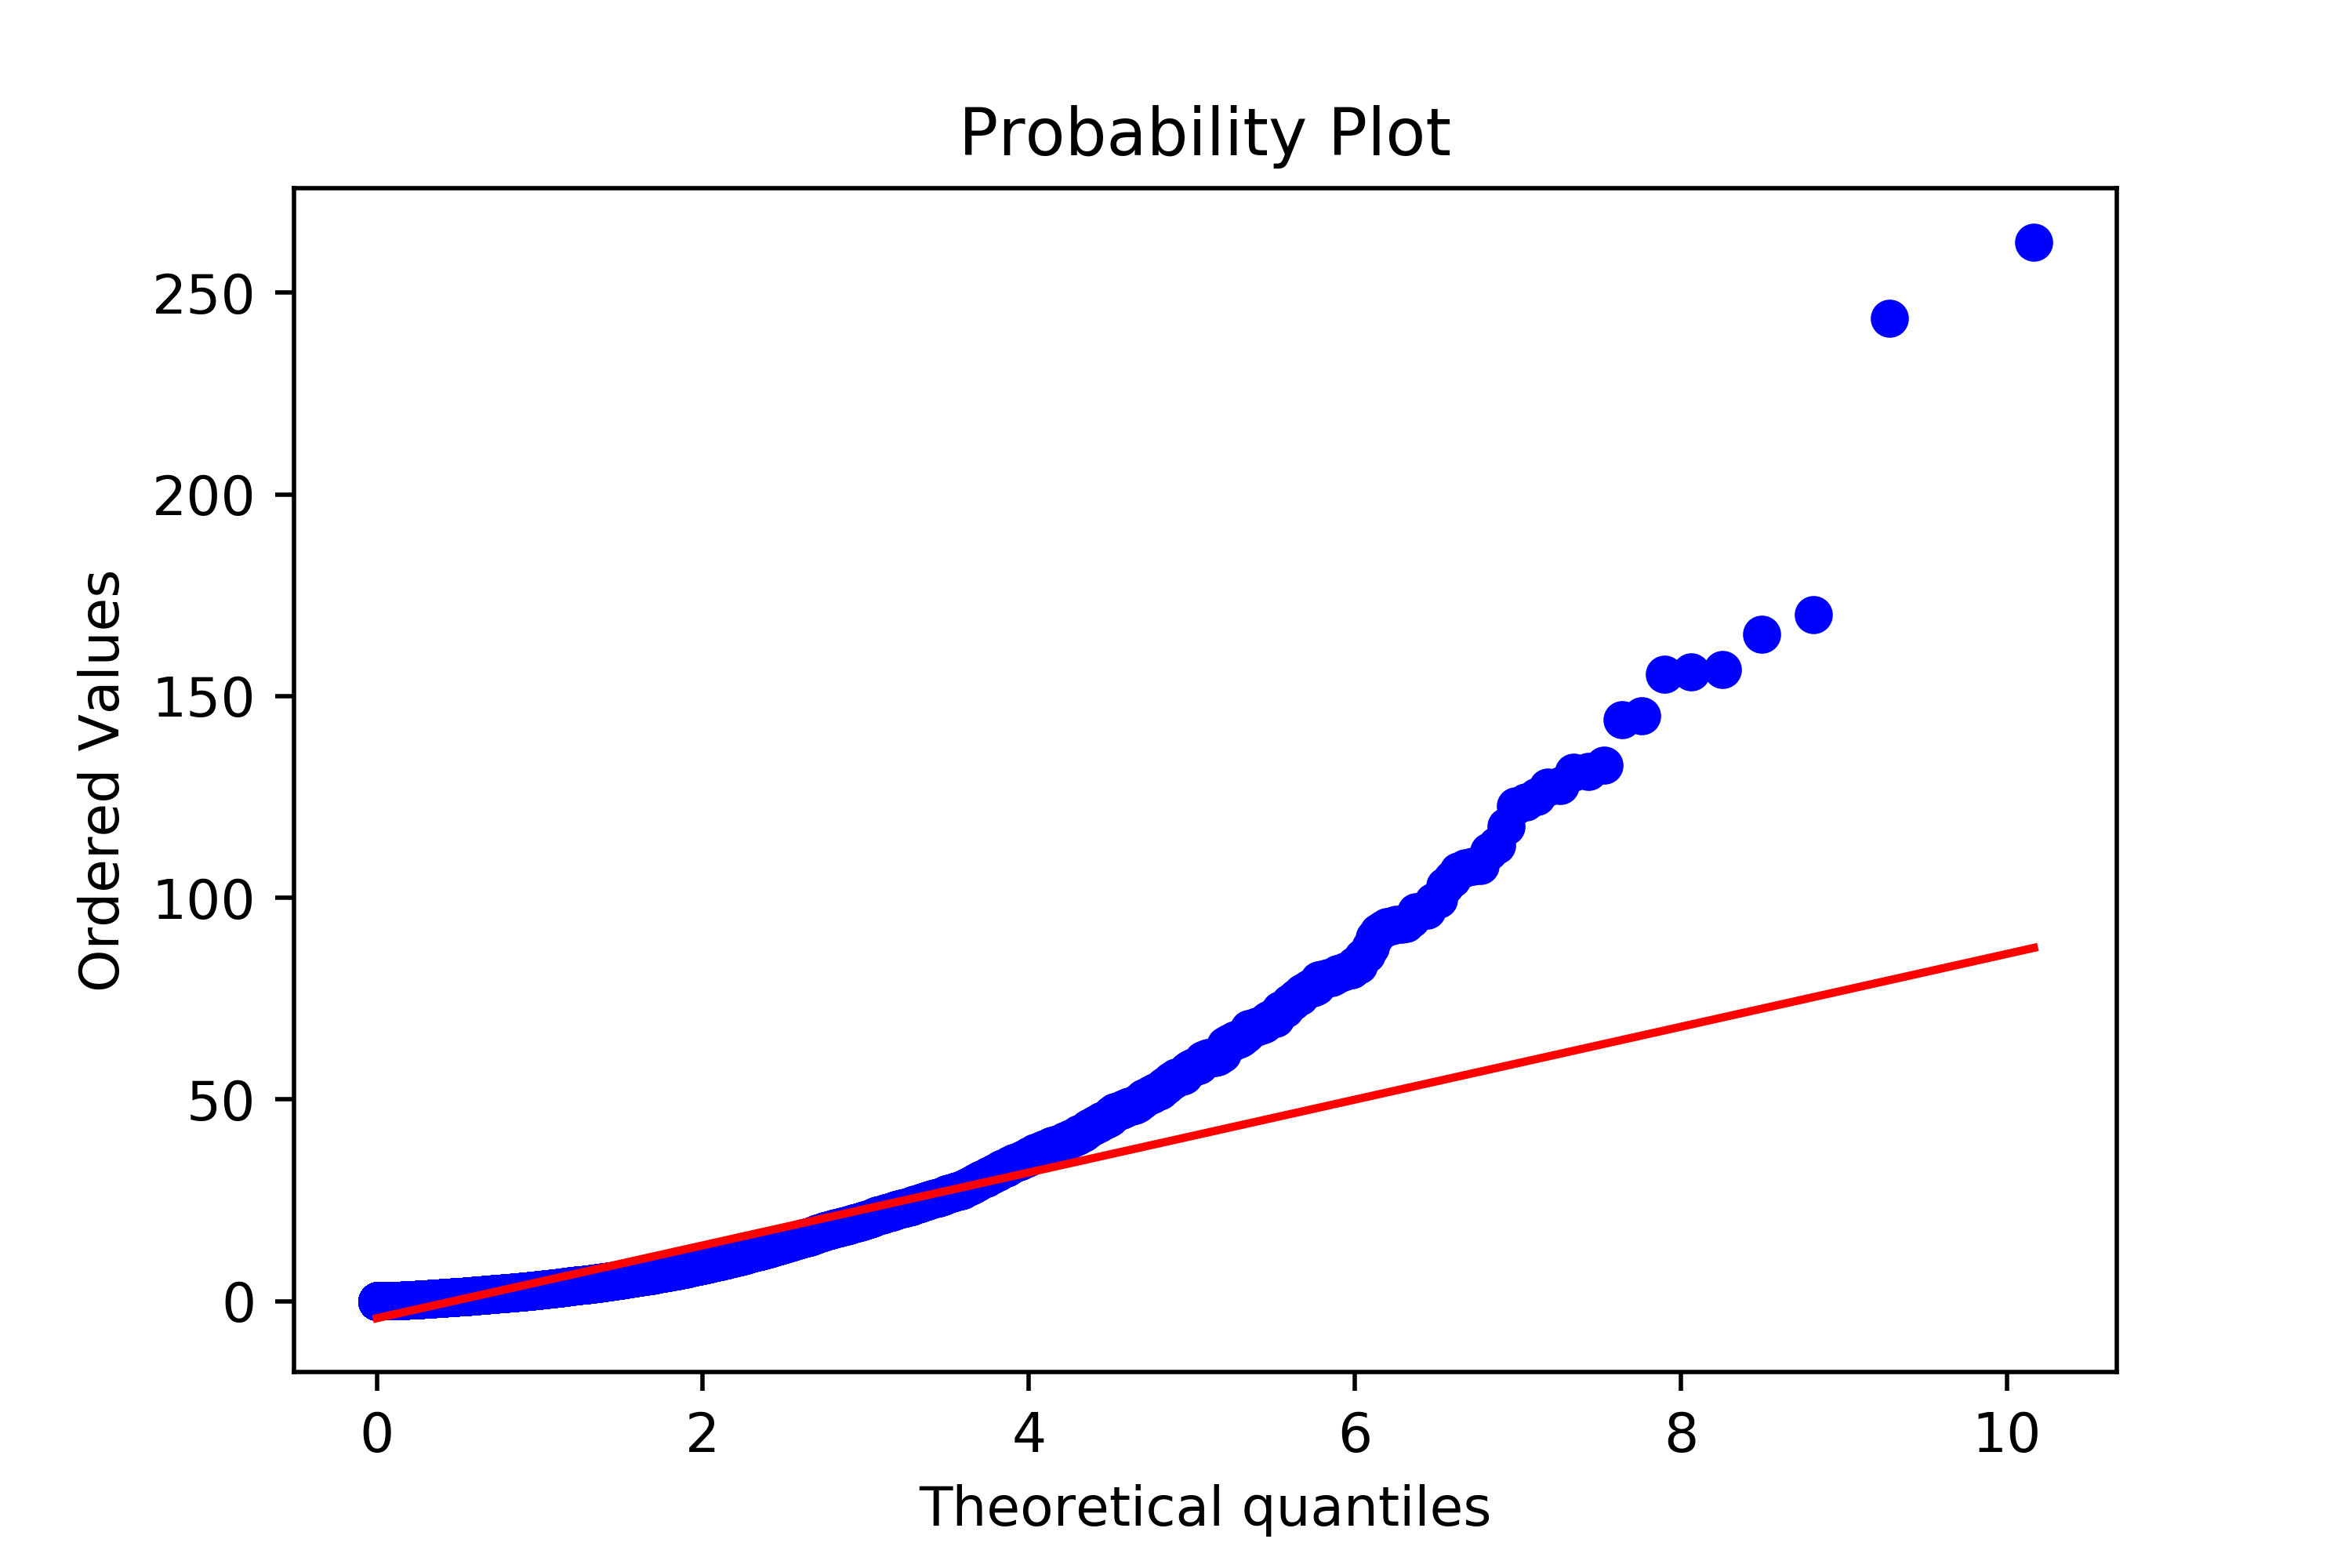
\includegraphics[width=60mm]{Figures/QQ_neg_k-1.png}}
{}
&
\subf{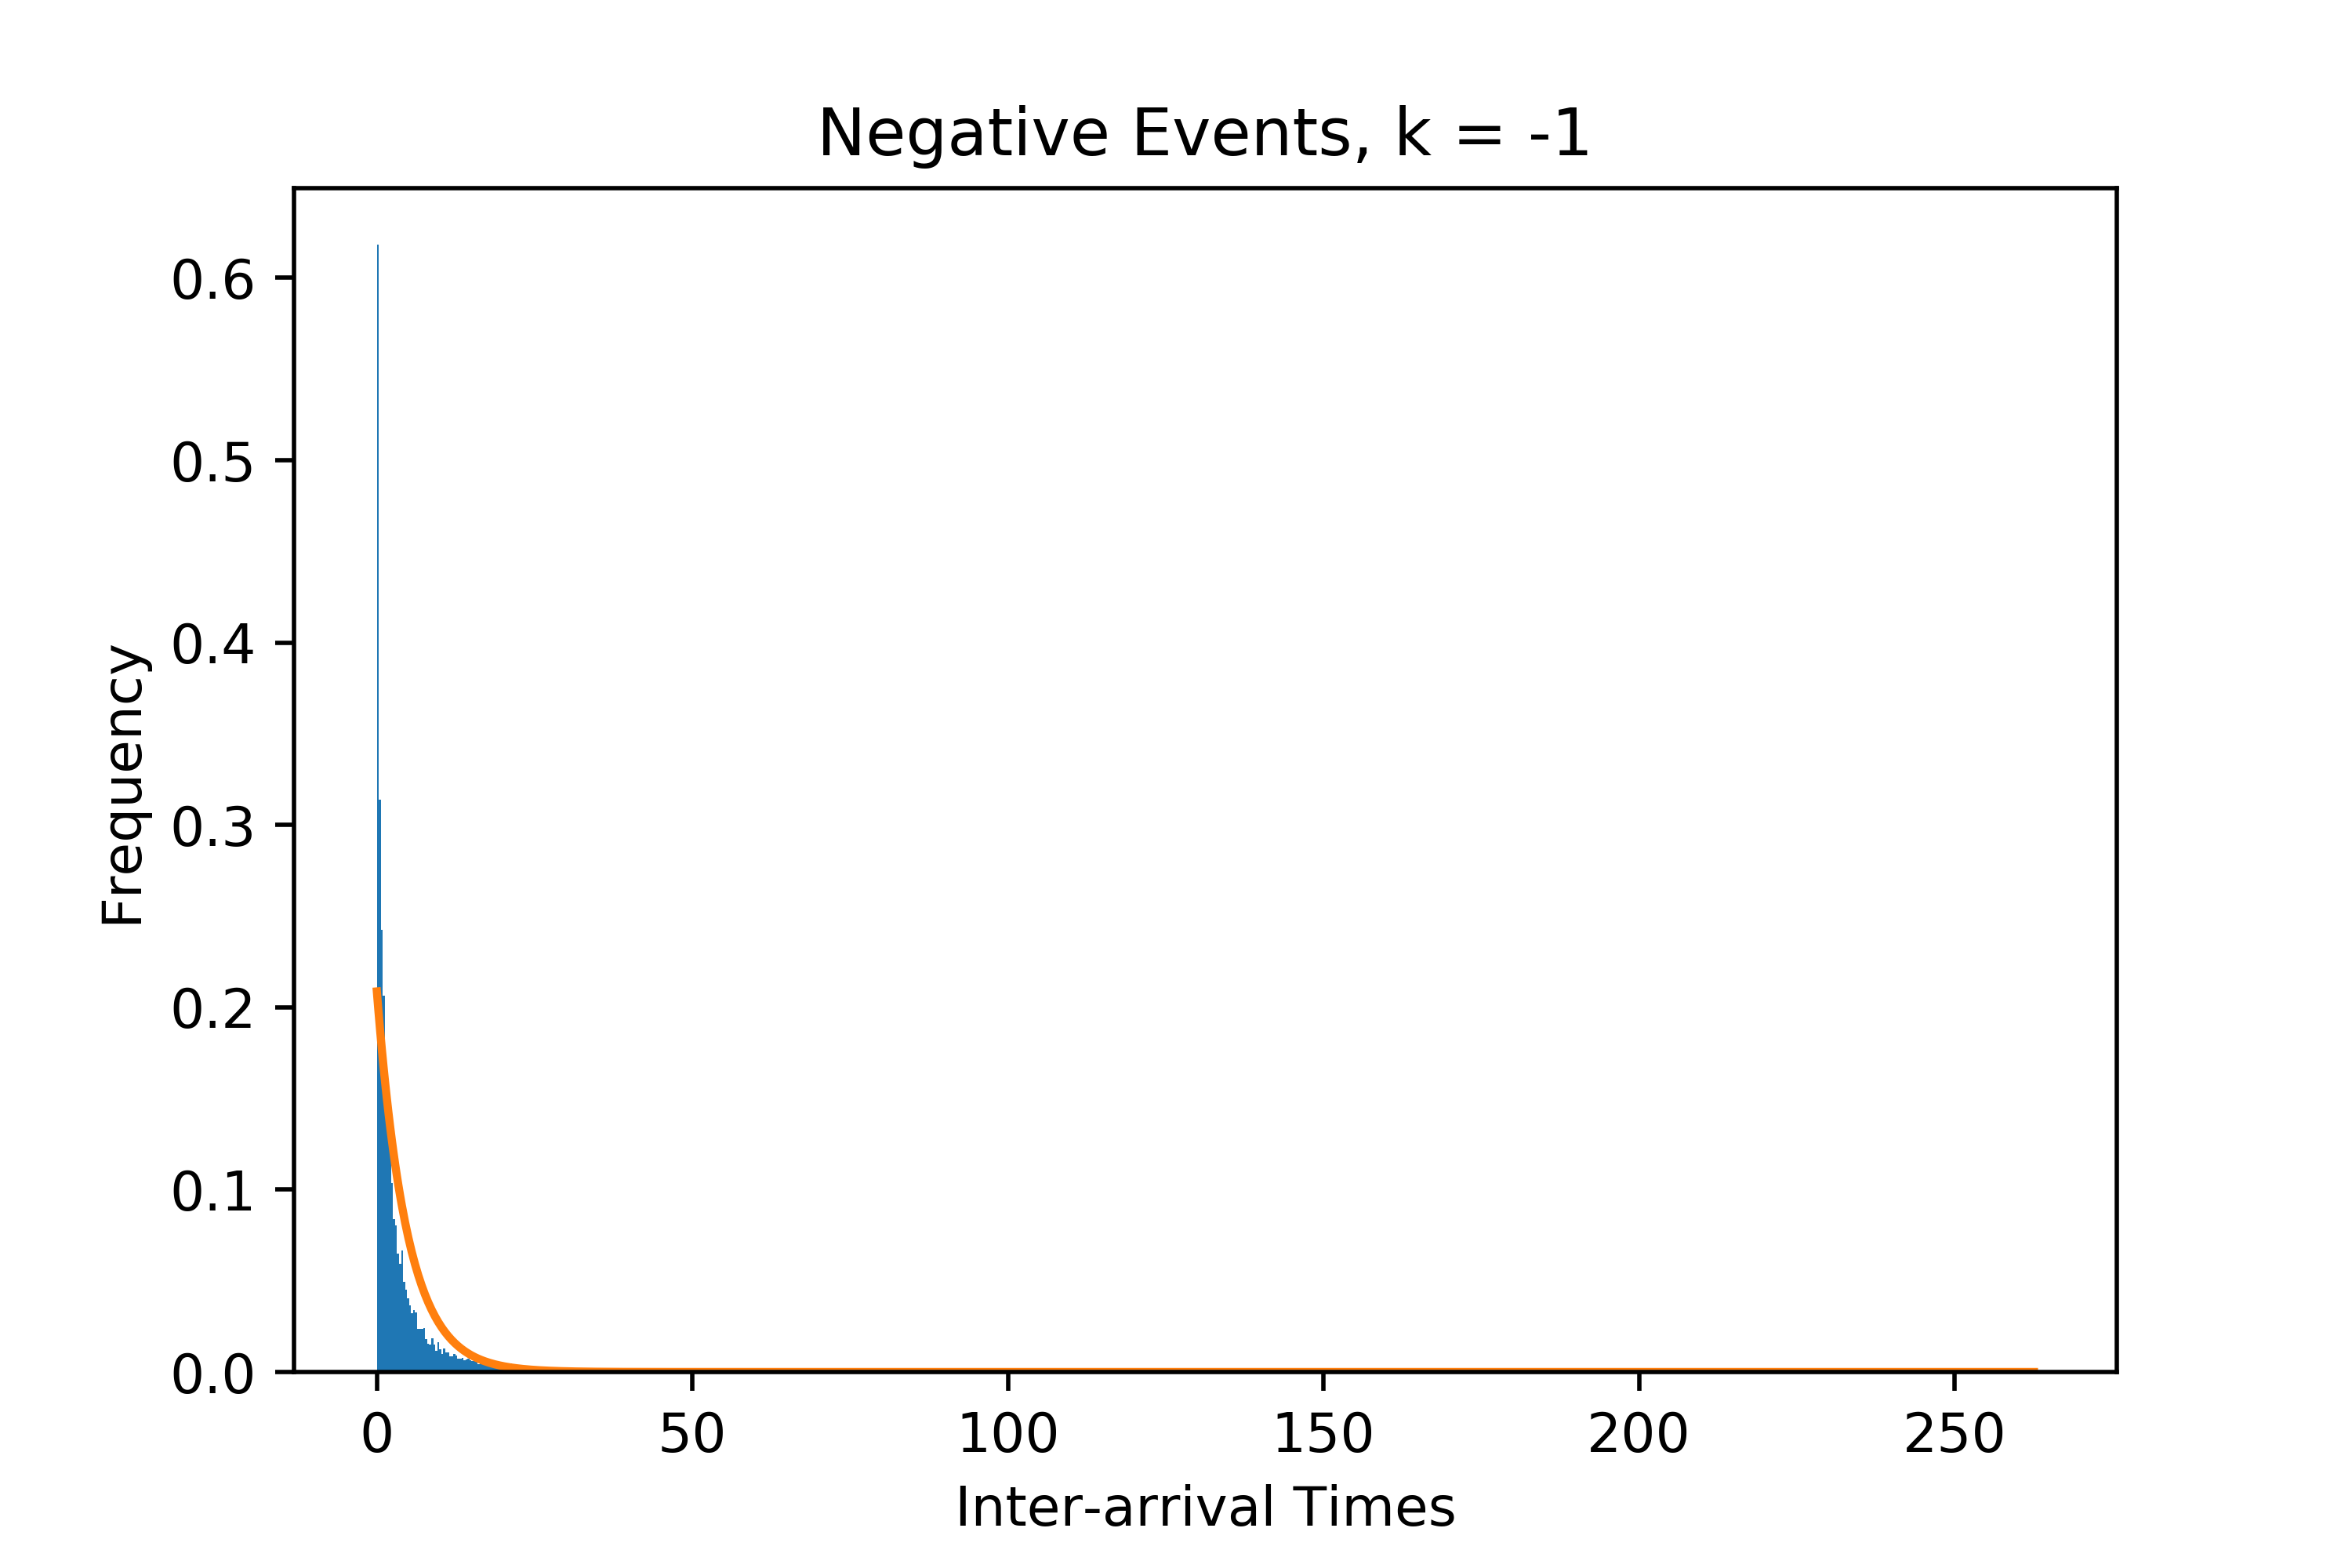
\includegraphics[width=60mm]{Figures/hist_neg_k-1.png}}
{}
\\
\subf{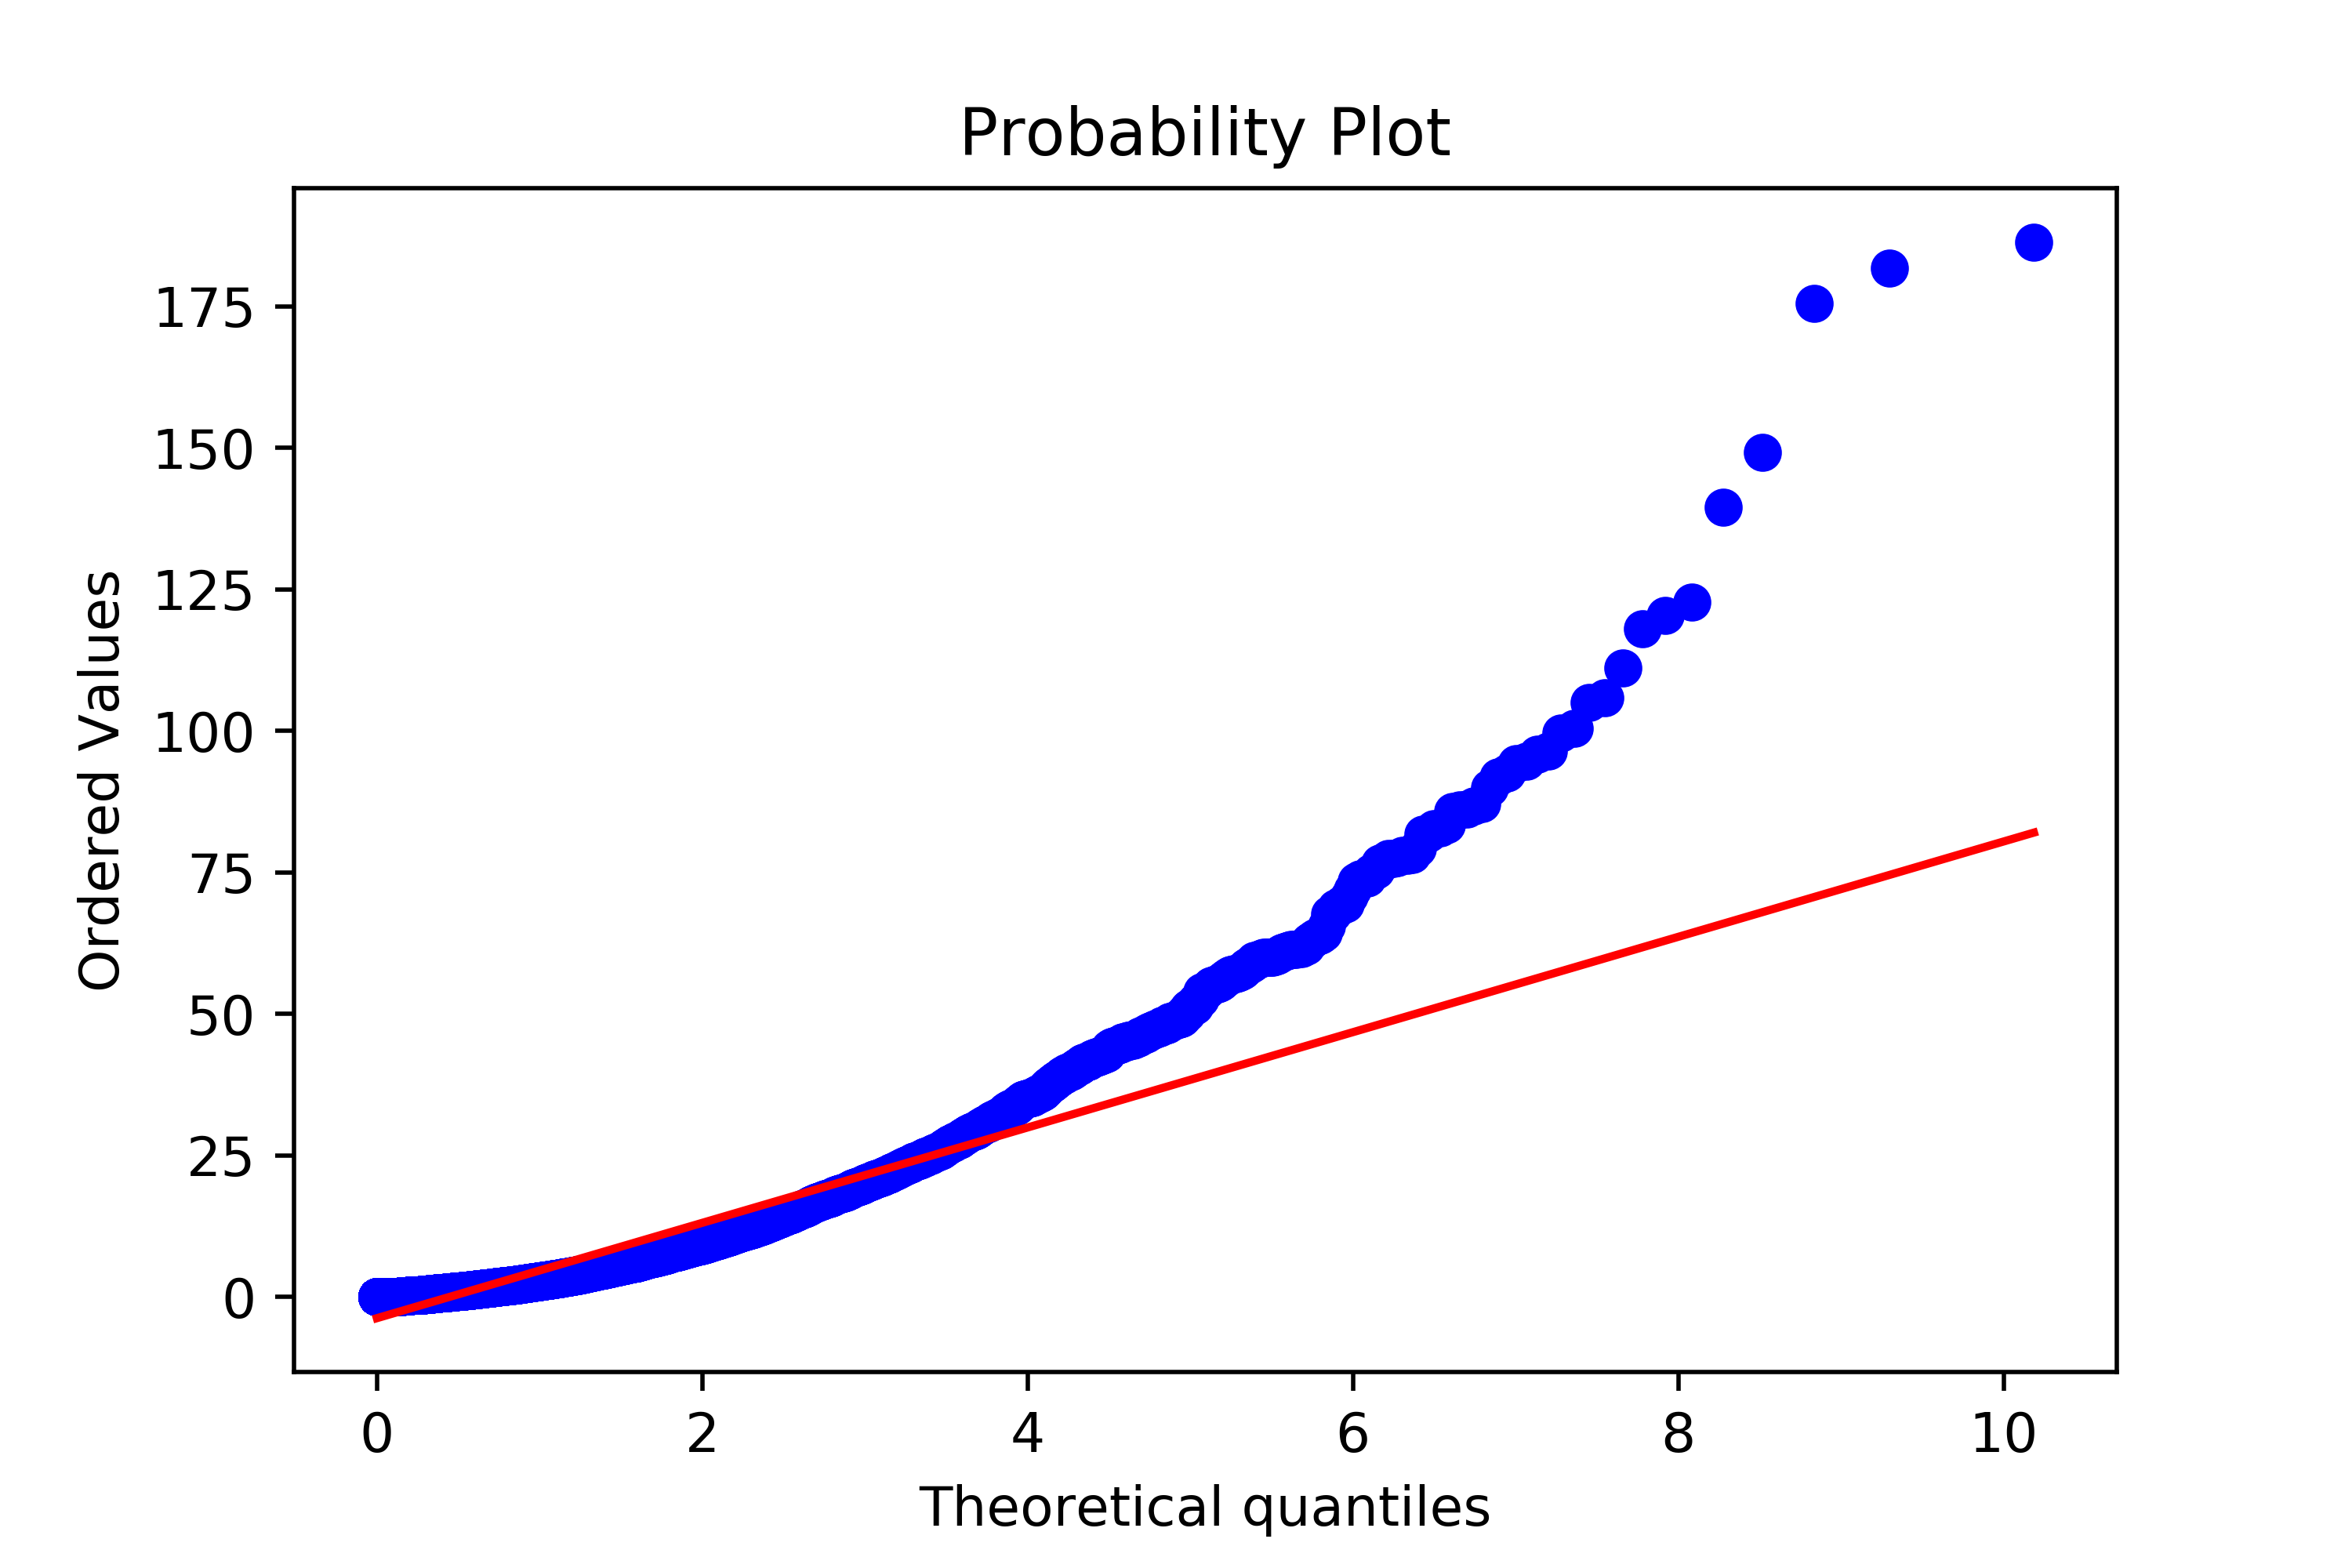
\includegraphics[width=60mm]{Figures/QQ_neg_k1.png}}
{}
&
\subf{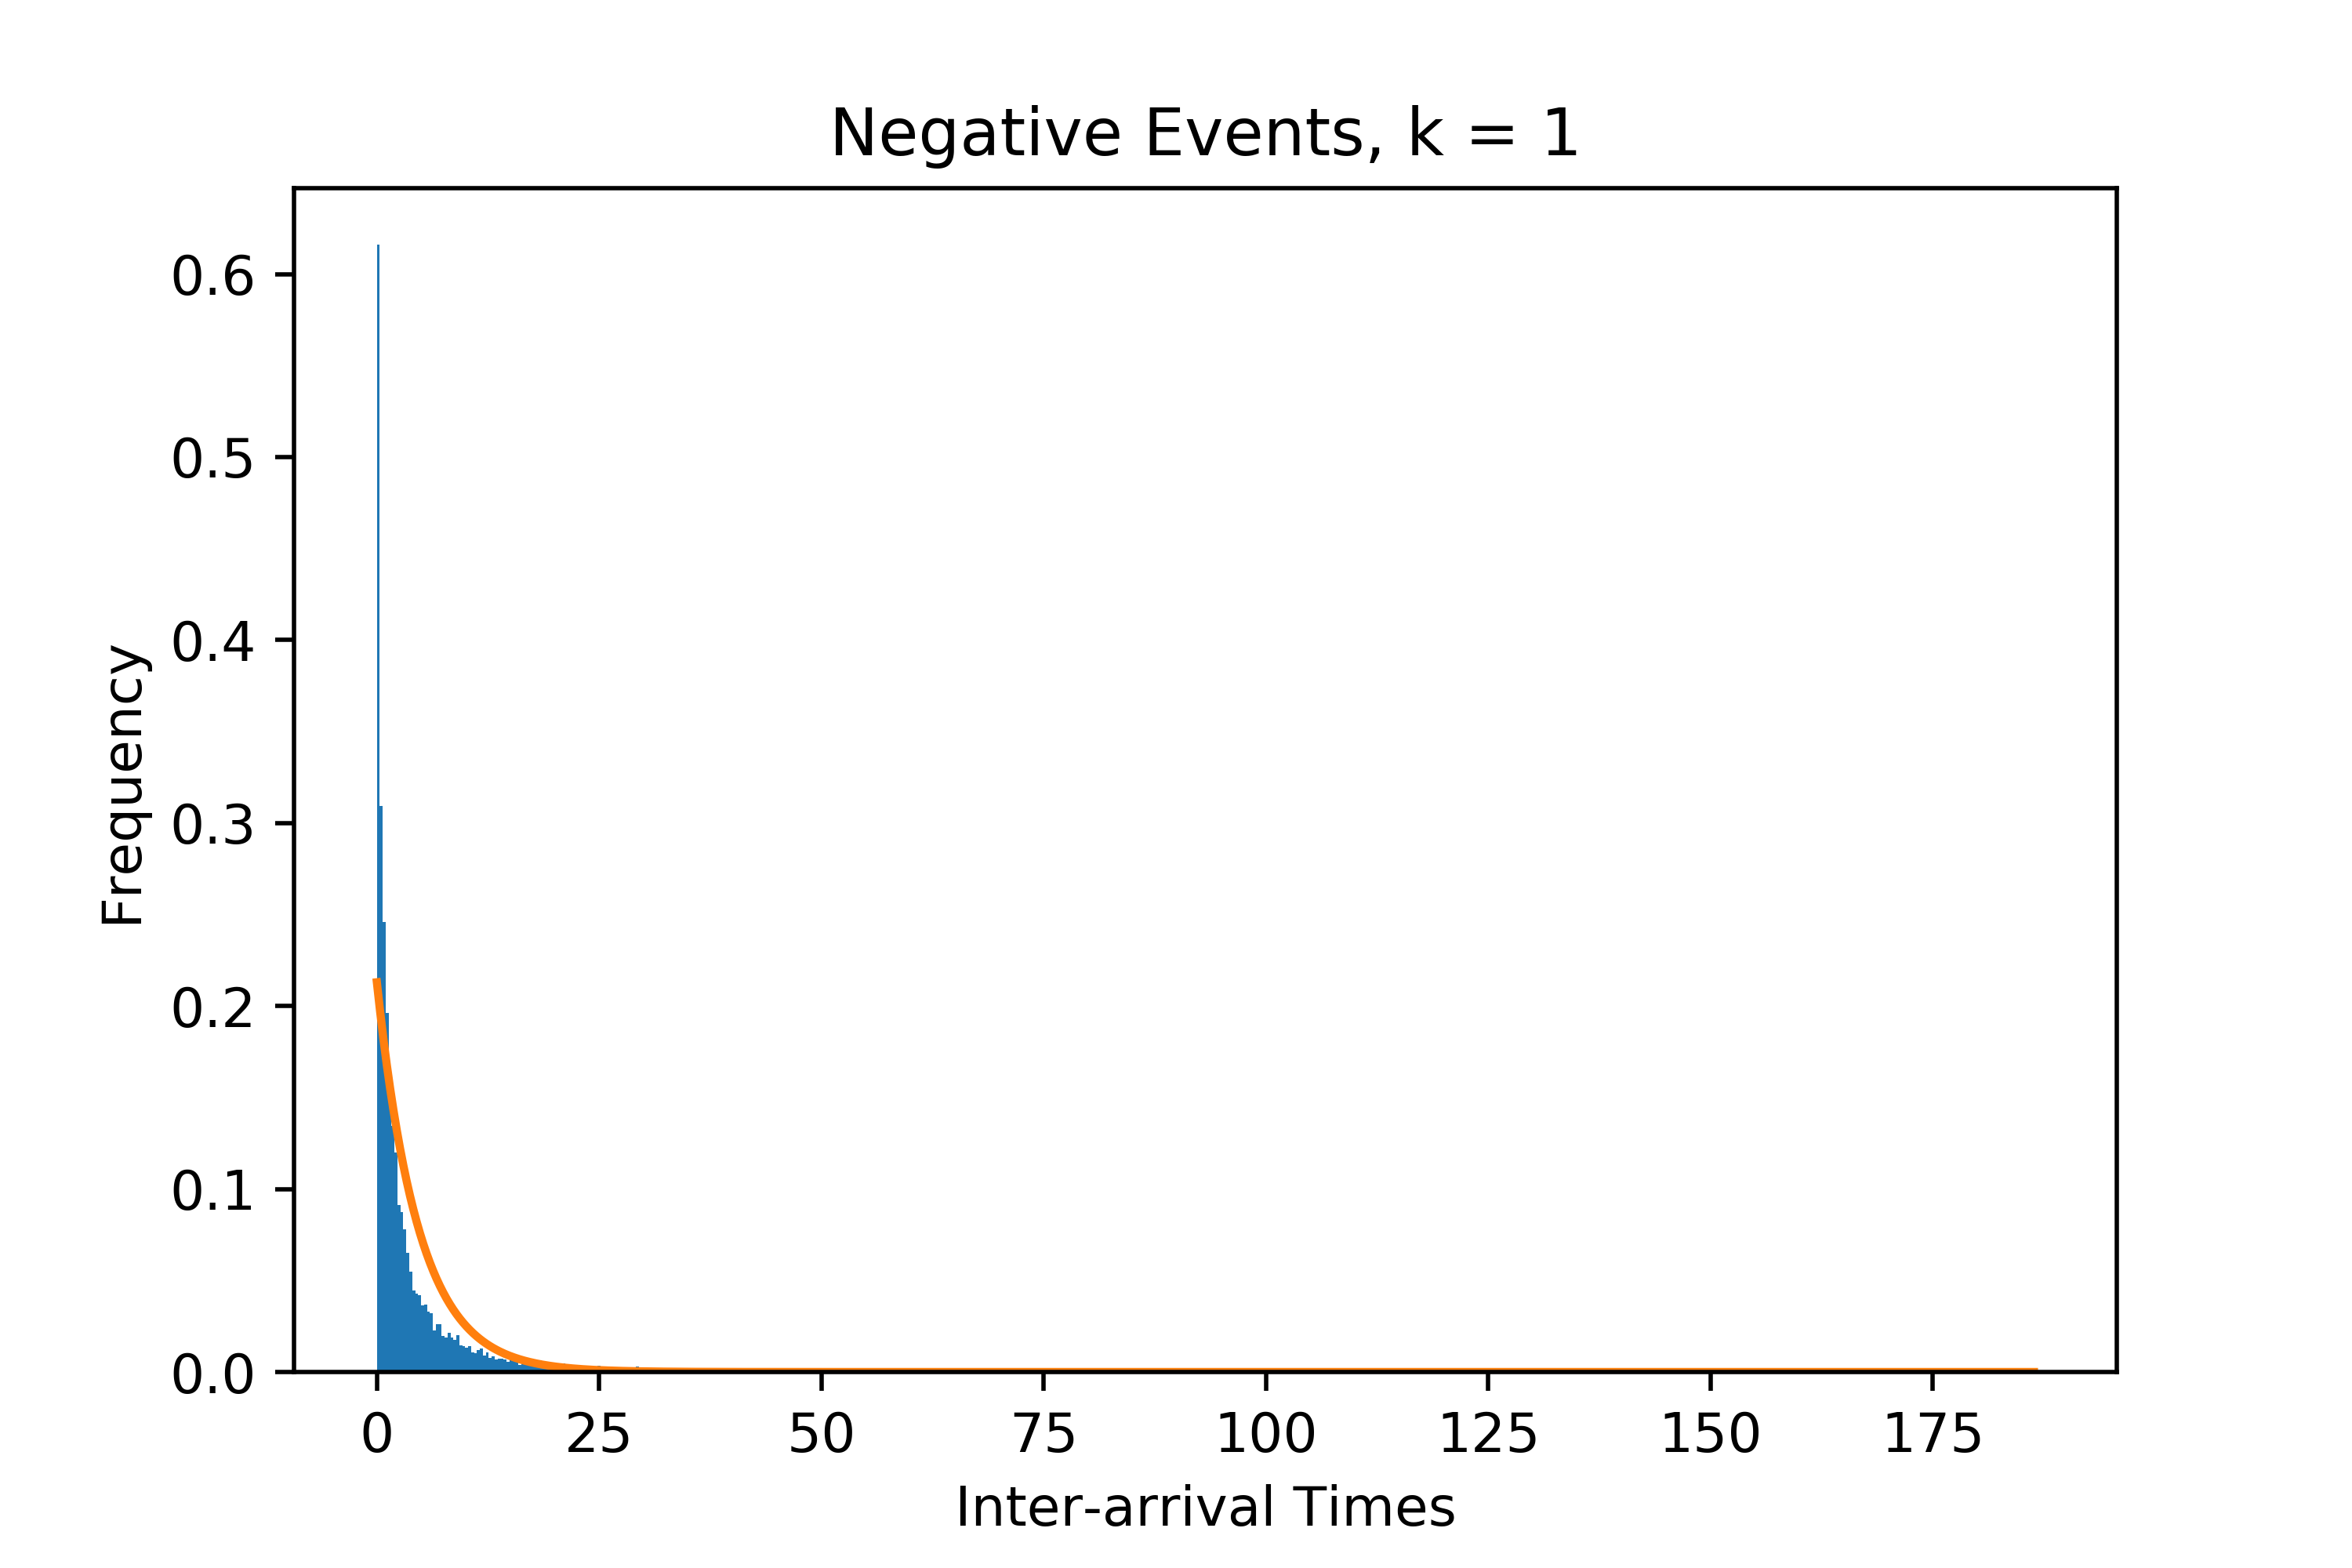
\includegraphics[width=60mm]{Figures/hist_neg_k1.png}}
{}
\\
\subf{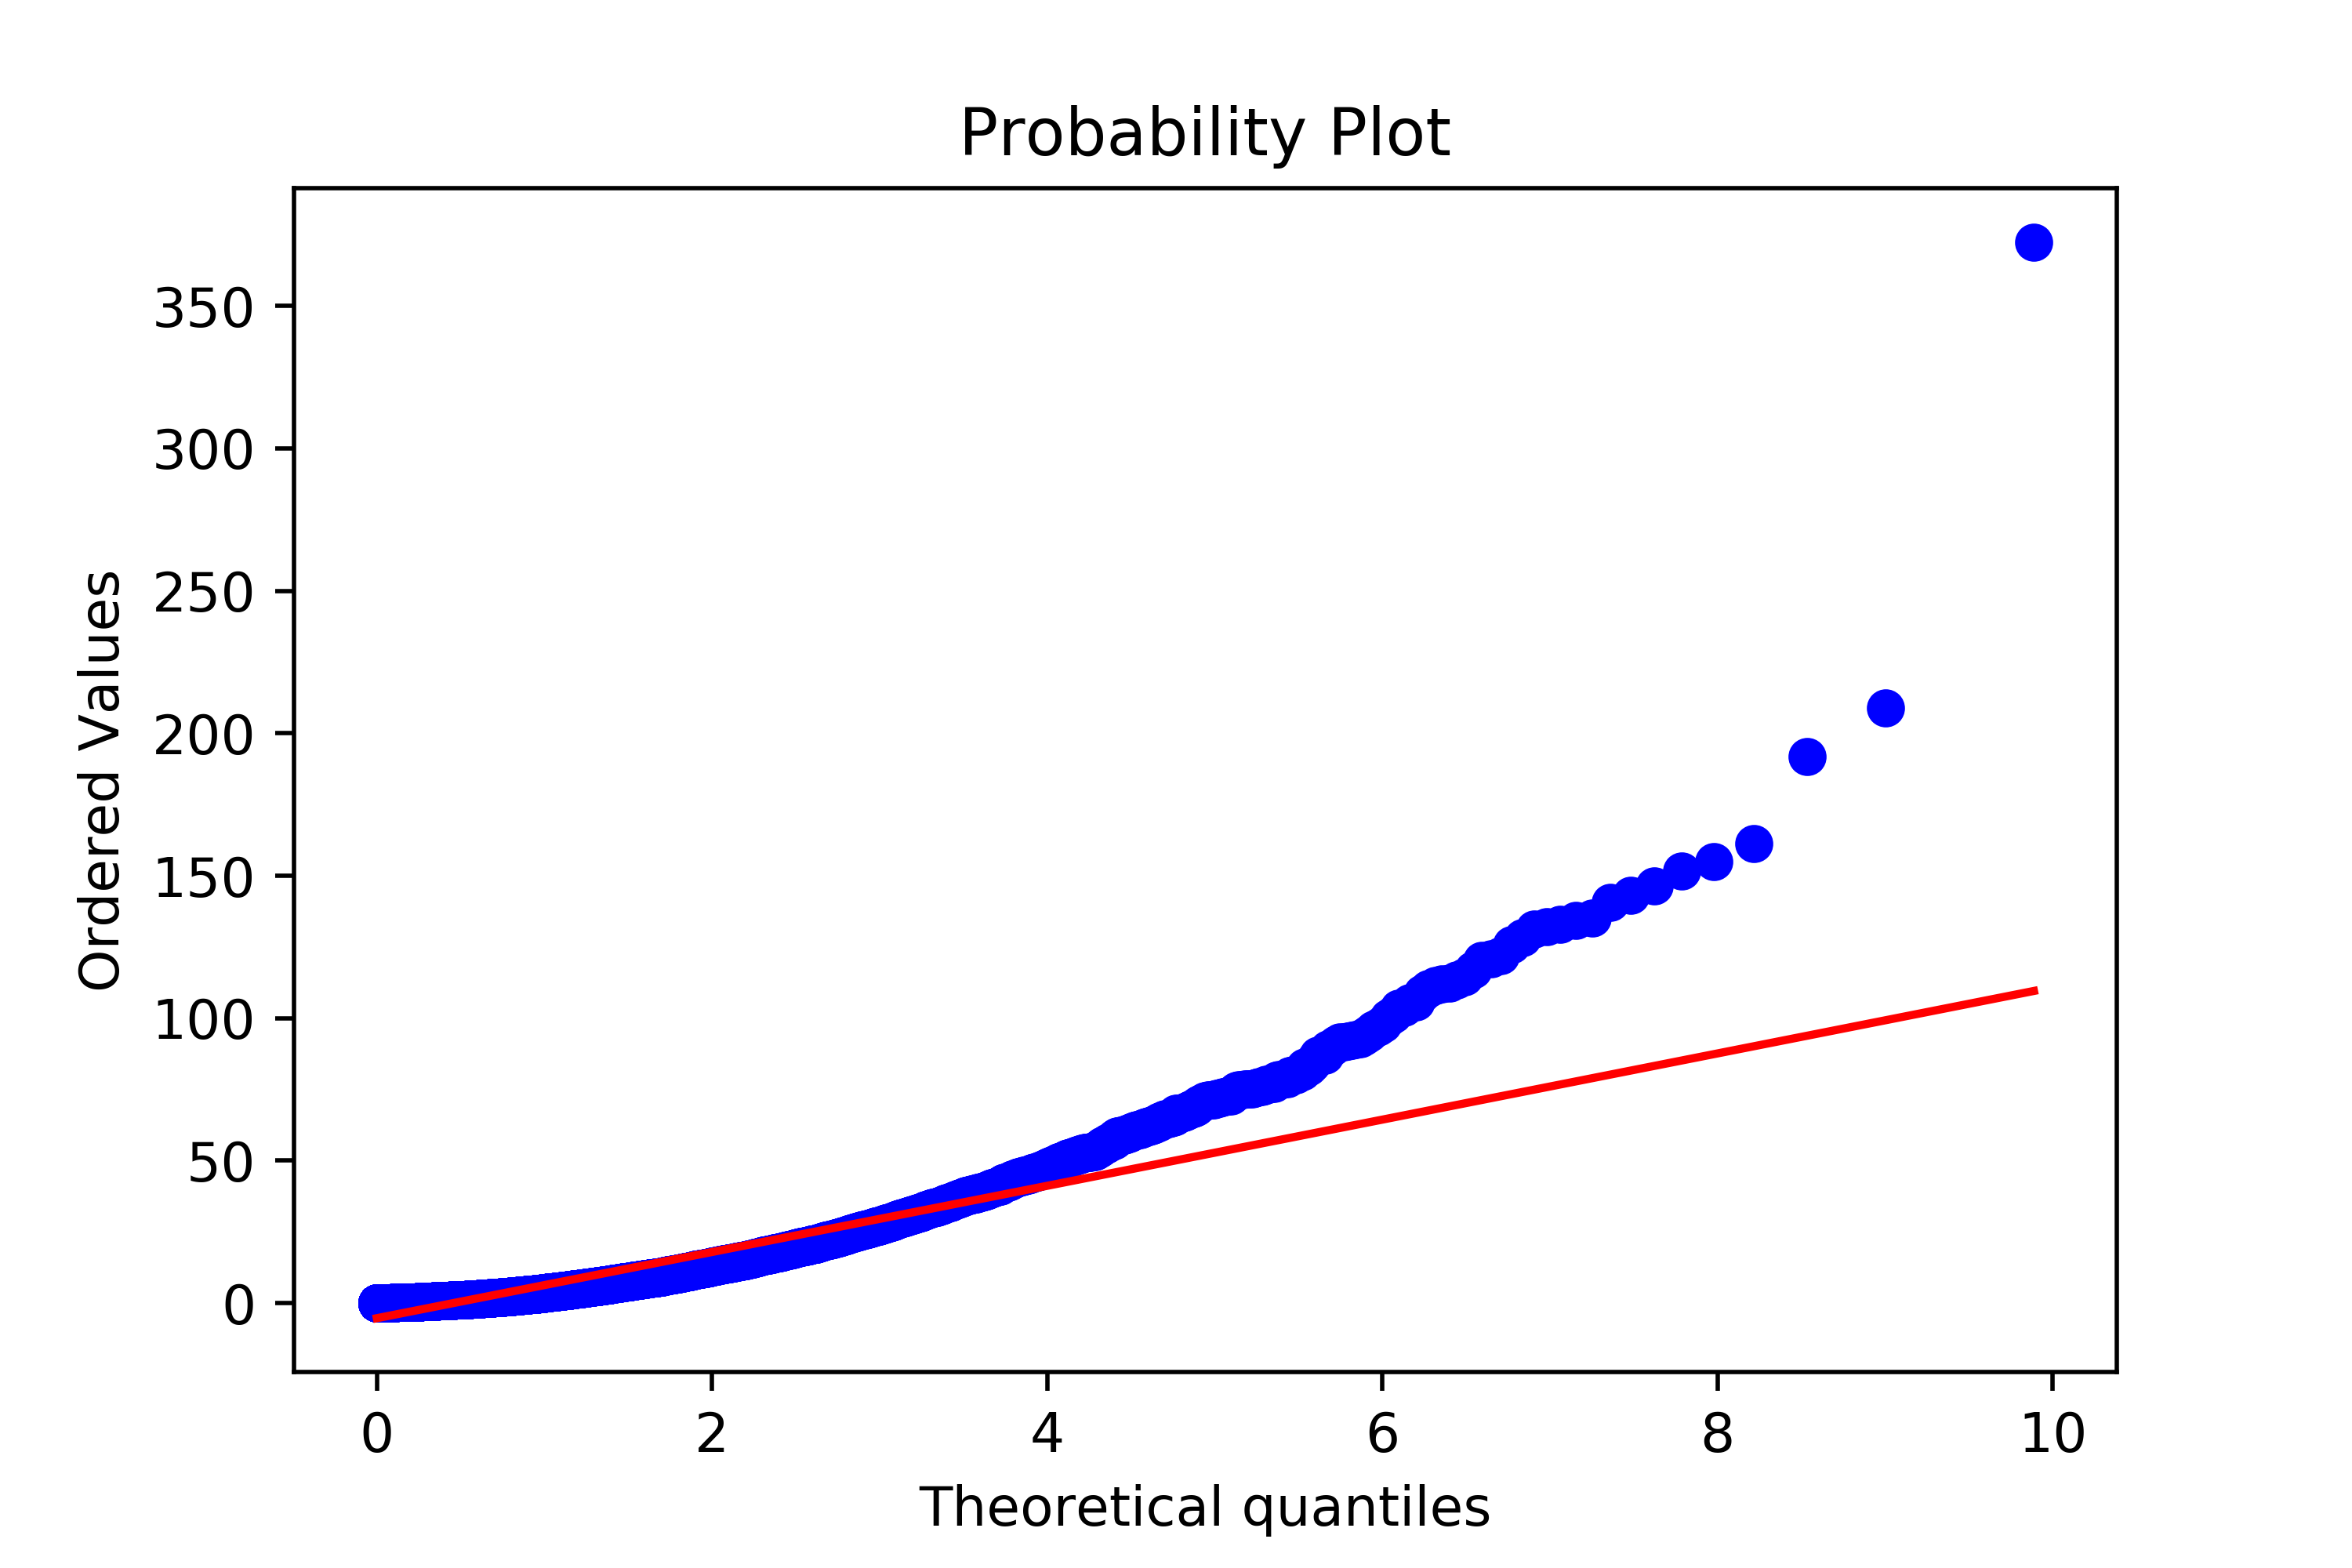
\includegraphics[width=60mm]{Figures/QQ_neg_k2.png}}
{}
&
\subf{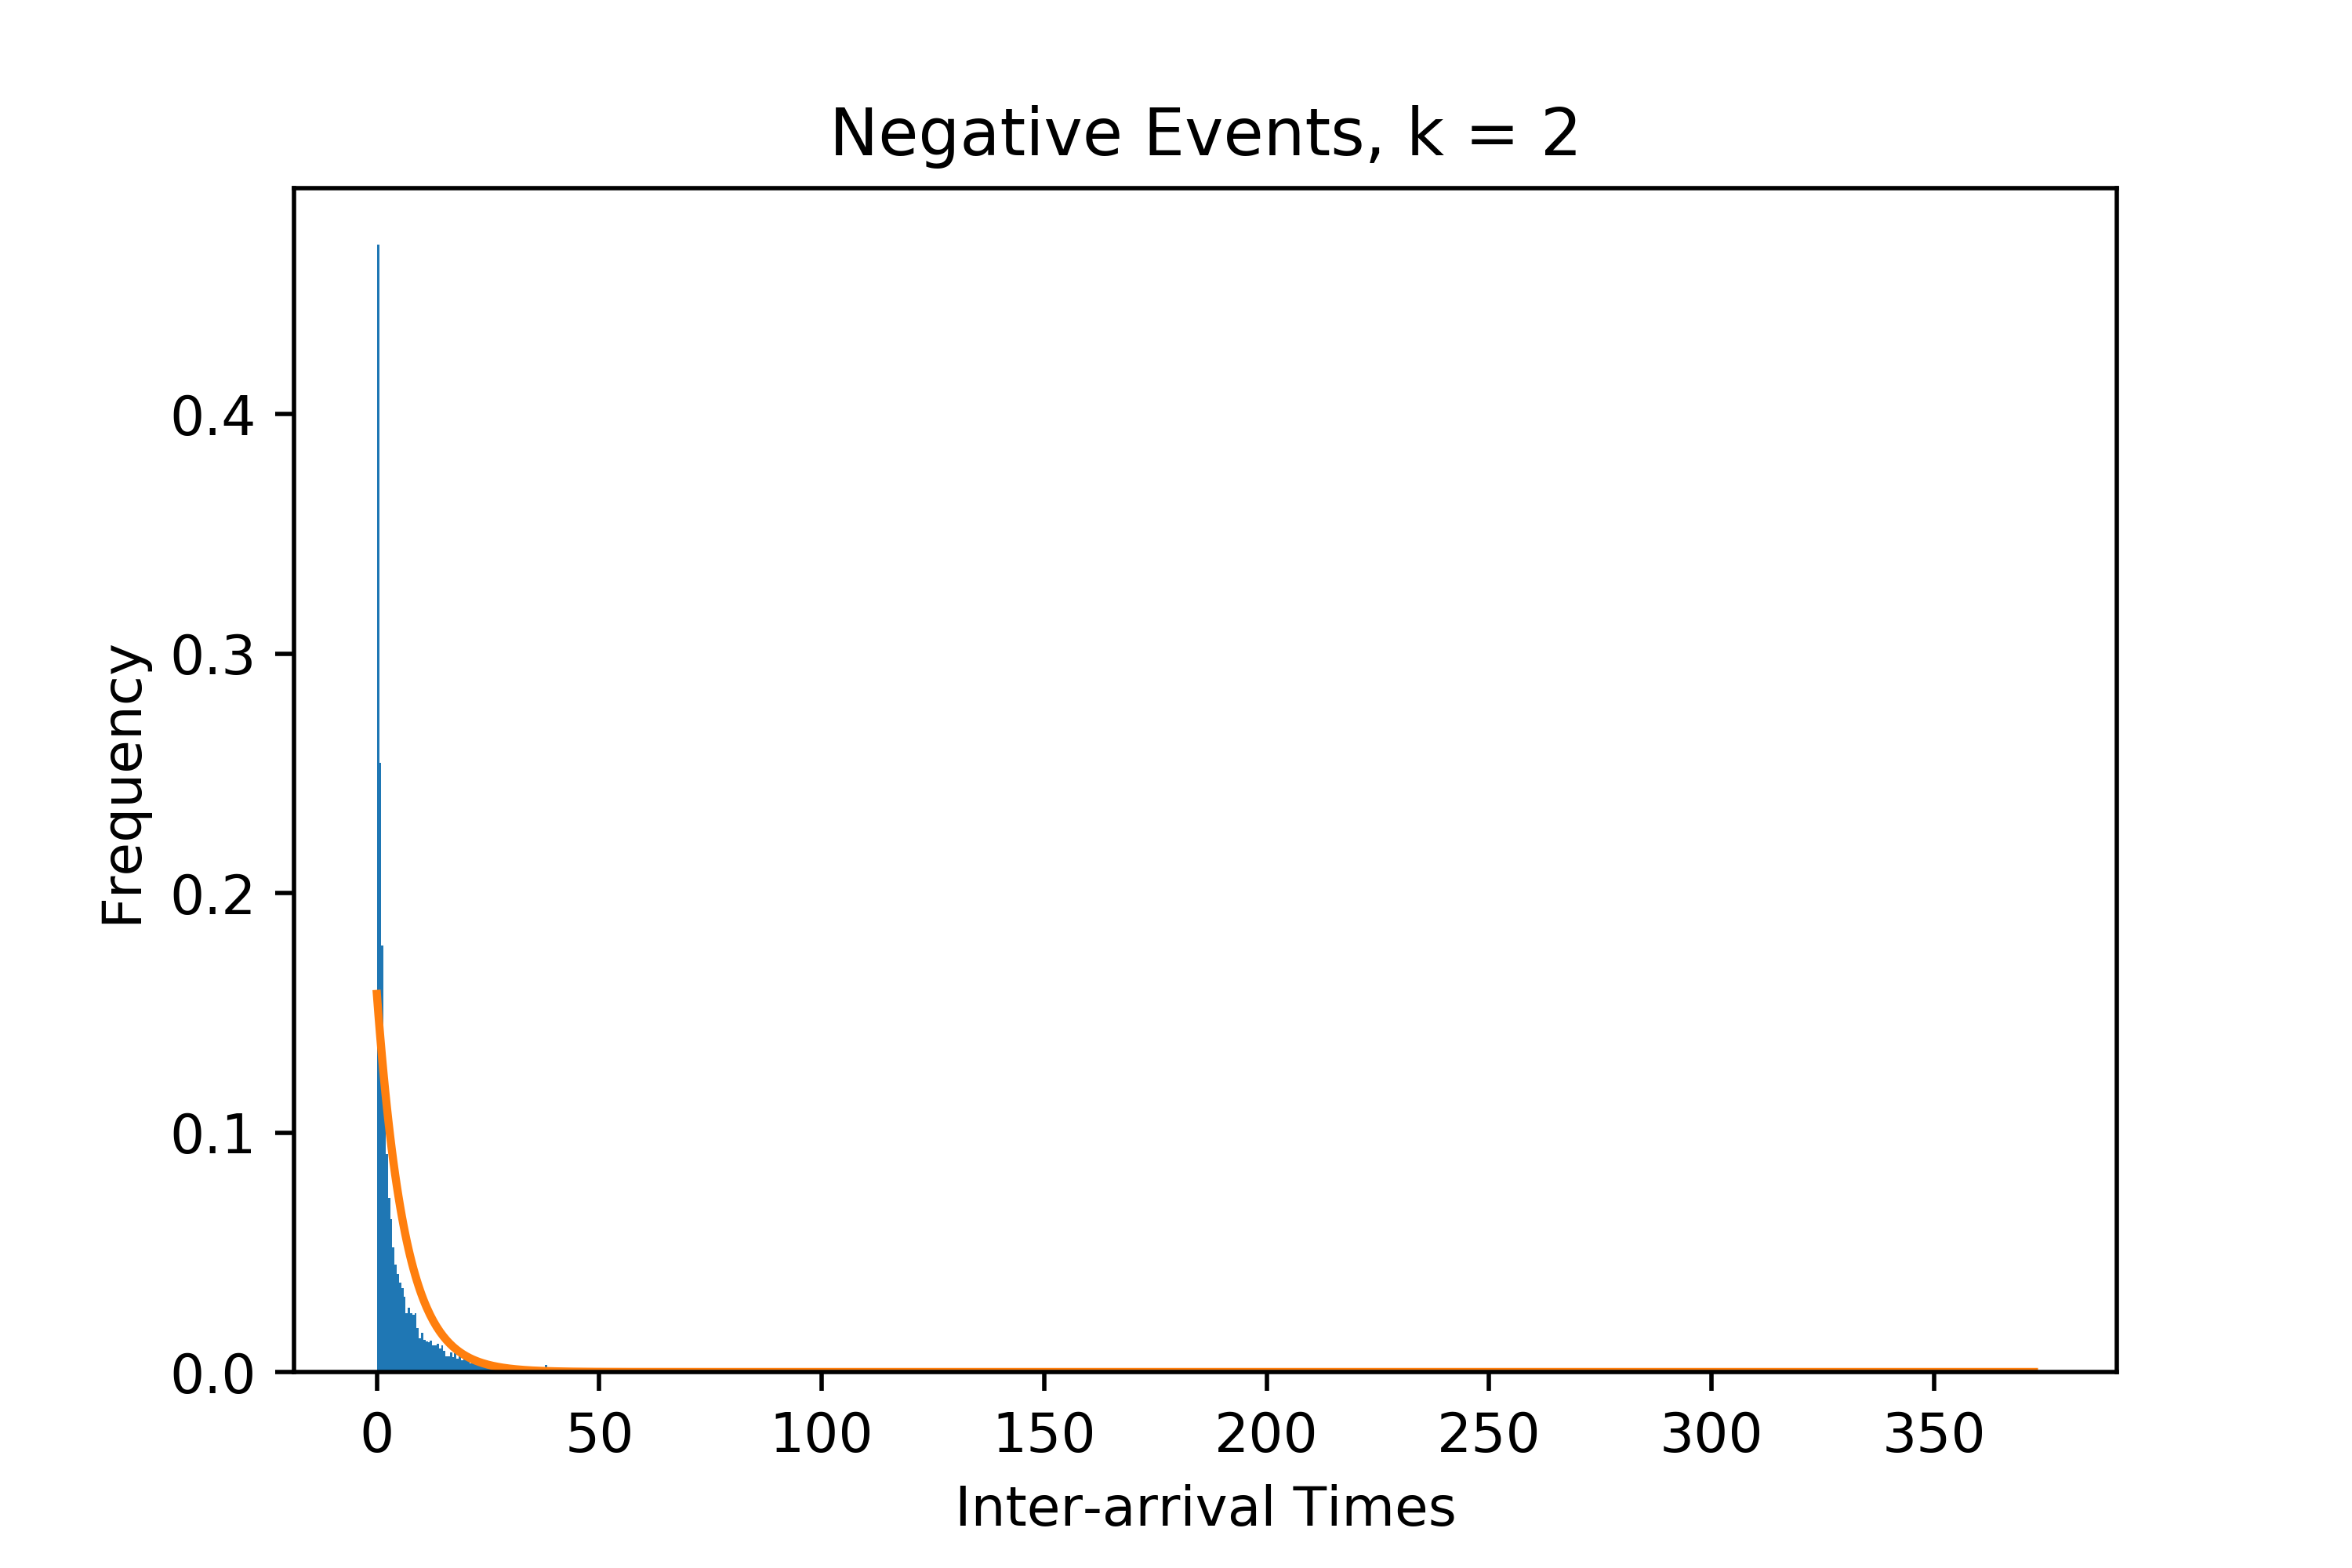
\includegraphics[width=60mm]{Figures/hist_neg_k2.png}}
{}
\\
\hline
\end{tabular}
\label{fig:interarrivals_neg}
\end{figure}

The products $\lambda^+_k \cdot \mu^+_k$ and $\lambda^-_k \cdot \mu^-_k$ can be thought of as the average rate of impact of positive and negative events at position $k$. In other words, they are the average positive and negative rates at which the size of the queue drifts over time. One concern with this model is that the impact of the positive events may overwhelm the impact of the negative events over time. That is, if $\lambda^+_k \cdot \mu^+_k > \lambda^-_k \cdot \mu^-_k$, then $Q^k(t)$ is unbounded as $t \to \infty$. This situation could arise due to trade imbalances in the time frame of the data that we use to estimate the parameters. We compare $\lambda^+_k \cdot \mu^+_k$ and $\lambda^-_k \cdot \mu^-_k$ in Table \ref{tab:parameters}. As can be seen, some rates are indeed larger for positive events compared to negative events. However, because the positive and negative rates are nearly the same at each position, $Q^k(t)$ should not increase an unreasonable amount in a short simulation time frame.

\section{Arrival Correlations}\label{ch:correlations}
Although each of the marginal processes can be individually modelled as a Poisson process, there were significant non-zero correlations between the numbers of arrivals at each position. Using a time period $t$ of 60 seconds, the correlations between $N^{\pm}_i(t)$ and $N^{\pm}_j(t)$ are used to generate a correlation matrix $R$ by sampling random intervals of length $t$ throughout the data collection period. With $K=10$, $R$ is a 40 x 40 matrix and is estimated with 160000 randomly selected intervals. The code written to estimate these correlations is found in Listing \ref{correlation-code}.

The correlation matrix for positive events is shown in Figure \ref{fig:pos_pos_corr_pic} where the entry $(i,j)$ is $\text{corr}(N^{+}_i(t), N^{+}_j(t))$. In general, there are high positive correlations between events at a position $k$ and positions $k \pm 1$, and to a lesser extent $k \pm 2$ and $k \pm 3$. The correlations between events near each other suggest that increased activity near a price influences similar activity for nearby prices. The smaller but significant positive correlations for positions far away from each other could be due to different levels of activity in the market at different times. For example, there may be more trading activity and therefore more events across the board during work hours vs. nighttime hours.

\begin{figure}[t]
\begin{center}
\caption{Correlation Matrix for $N^{+}_i(t), N^{+}_j(t)$, $t$ = 60 seconds}
\label{fig:pos_pos_corr_pic}
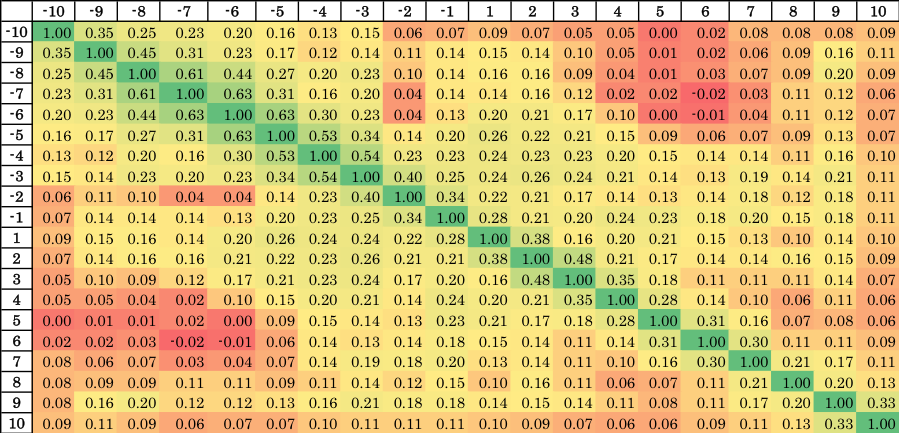
\includegraphics[width=\textwidth]{LaTeX/Figures/pos_pos_correlations.png}
\end{center}
\end{figure}

The correlation matrix for positive vs. negative events is shown in Figure \ref{fig:pos_neg_corr_pic} where the entry $(i,j)$ is $\text{corr}(N^{+}_i(t), N^{-}_j(t))$. Particularly notable is the very high (nearly 1) correlation between positive and negative at the same position. This characteristic could be due to traders reacting to updates by placing orders in the opposite direction, and could indicate that the order book is resilient to changes in the short term.

\begin{figure}[t]
\caption{Correlation Matrix for $N^{+}_i(t), N^{-}_j(t)$, $t$ = 60 seconds}
\begin{center}
\label{fig:pos_neg_corr_pic}
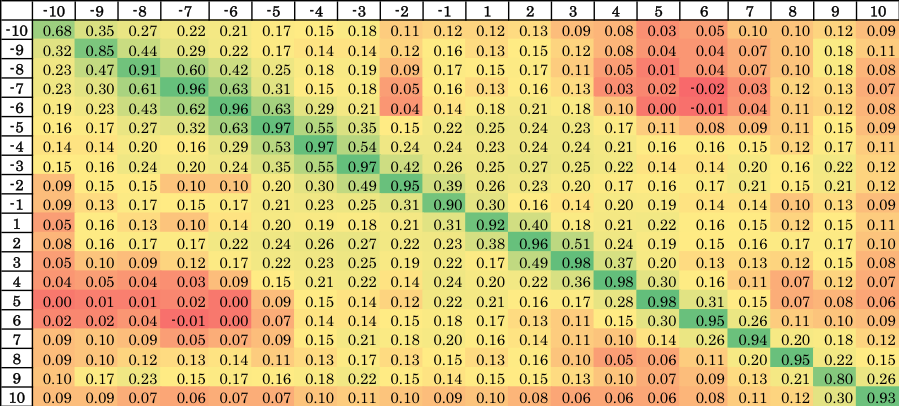
\includegraphics[width=\textwidth]{LaTeX/Figures/pos_neg_correlations.png}
\end{center}
\end{figure}

The correlation matrix for negative events is shown in Figure \ref{fig:neg_neg_corr_pic} where the entry $(i,j)$ is $\text{corr}(N^{-}_i(t), N^{-}_j(t))$. This matrix is similar in nature to the one for positive events, where positions near each other exhibit high correlations and there are lower positive correlations between positions that are further away from each other.

\begin{figure}[t]
\begin{center}
\caption{Correlation Matrix for $N^{-}_i(t), N^{-}_j(t)$, $t$ = 60 seconds}
\label{fig:neg_neg_corr_pic}
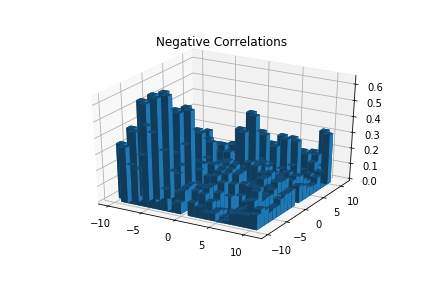
\includegraphics[width=\textwidth]{LaTeX/Figures/neg_neg_correlations.png}
\end{center}
\end{figure}

These non-zero correlations are clearly non-negligible, so a multivariate Poisson process where the arrivals are correlated and the marginal arrivals follow single Poisson processes is appropriate. The correlations in Figures \ref{fig:pos_pos_corr_pic}, \ref{fig:pos_neg_corr_pic}, and \ref{fig:neg_neg_corr_pic} can be combined to form $R$ as described. The procedure for simulating the multivariate Poisson process is discussed in Chapter \ref{ch:simulation}.
